\title{Pipeline Dalio}
\author{Duncan Palmer}
\date{}

\documentclass[12pt]{article}
\usepackage[top=0.85in,left=0.85in,right=0.85in,footskip=0.75in]{geometry}
\usepackage{parskip}
\usepackage{amsmath}
\usepackage{mathrsfs}
\usepackage{amssymb}
\usepackage{graphicx}
\usepackage{mathtools}
\usepackage{subfig}
\usepackage{listings}
\usepackage[T1]{fontenc}

\usepackage{graphics}
\usepackage{float}

\usepackage{cite}
\usepackage{tabulary}
\usepackage{setspace}
\usepackage{booktabs}
\usepackage{parskip}
\usepackage{hhline}
\usepackage{color}
\usepackage{authblk}
% \usepackage{ccaption}
\usepackage{enumerate}
\usepackage[usenames,dvipsnames,svgnames,table]{xcolor}
\usepackage{subfig}
\usepackage{xr-hyper} 
\usepackage{hyperref}
\usepackage{xcolor}

\hypersetup{
     colorlinks = true,
     citecolor = gray,
     linkcolor = NavyBlue
}

\begin{document}
\graphicspath{{../../../QC_plots/sample_plots/}{../../../QC_plots/variant_plots/}}
\maketitle
\begin{itemize}
	\item Filter GT content from joint called .vcf. Throw away the following (01\_load\_vcf\_filterGT.py):
	\begin{itemize}
		\item If hom ref, at least one of:
		\begin{itemize}
			\item (ref allele depth)/depth $< 0.8$
			\item genotype quality $< 20$
			\item depth $< 10$
		\end{itemize}
		\item If het, at least one of:
		\begin{itemize}
			\item (ref allele depth + alt allele depth)/depth $< 0.8$
			\item (alt allele depth)/depth $< 0.2$
			\item ref phred-scaled genotype posterior $< 20$
			\item depth $< 10$
		\end{itemize}
		\item If hom var, at least one of:
		\begin{itemize}
			\item (alt allele depth)/depth $< 0.8$
			\item ref phred-scaled genotype posterior $< 20$
			\item depth $< 10$
		\end{itemize}
    \end{itemize}
    \item Using 02\_prefilter\_variants.py, Remove variants that either:
    \begin{itemize}
    	\item Did not fall in the target intervals
    	\item Fall in a low complexity region
    	\item Have VQSLOD $< -8$
    \end{itemize}
    \item Using 03\_initial\_sample\_qc.py, run `sample\_qc' using hail and remove (see Figure \ref{fig:initial_sample_qc}):
    \begin{itemize}
    	\item sample call rate $< 0.9$
    	\item FREEMIX contamination (\%?) $> 0.004$
    	\item PCT\_CHIMERAS (\%?) $>  0.0015$
    	\item mean depth (dpMean) $< 30$
    	\item mean genotype quality (gqMean) $< 82.5$
    \end{itemize}
    Thresholds used were based on plotting the various distributions.
    \item Export common variants (allele frequency between 0.01 to 0.99) with high call rate ($>0.98$) to plink format and prune to independent SNPs using `--indep 50 5 2'
	\item Impute the sexes of the individuals (`05\_impute\_sex.py'; see Figure \ref{fig:impute_sex}) with this pruned set of variants on the X, and create list of samples with incorrect or unknown sex as defined by:
	\begin{itemize}
		\item Sex is `unknown' in the phenotype files.
		\item F-statistic $> 0.6$ and the sex is `female' in the phenotype file.
		\item F-statistic $< 0.6$ and the sex is `male' in the phenotype file.
		\item Currently I don't add individuals to this list based on number of calls in the Y - perhaps I should add this.
	\end{itemize}
	\item Compute IBD between all pairs of individuals using the pruned set of variants in the autosomes (`06\_ibd.py'; see Figure \ref{fig:IBD_plot}).
		\begin{itemize}
			\item Create sample list of individuals such that no pair has $\hat{\pi}>0.2$.
		\end{itemize}
	\item Run PCA on samples after removing relateds and those that passed initial QC, using the pruned set of variants (`09\_pca.py'; see Figure \ref{fig:PCA}).
	\item Run PCA on samples plus all of 1000 genomes (`10\_pca\_1kg.py'; see Figure \ref{fig:PCA_1kg}).
	\begin{itemize}
		\item Train a random forest (500 trees) on the super populations of 1000 genomes and predict super populations of Dalio samples.
		\item Denote strictly defined European subset as those with probability $> 0.9$ of being European according to the classifier. 
	\end{itemize}
	\item Run PCA on samples restricted to the strictly defined European subset, and check for outliers (`11\_pca\_EUR.py'; see Figure \ref{fig:PCA_EUR}).
	\item Using a much looser definition of European, restrict to US samples from MGH and Johns Hopkins, and run PCA (`12\_pca\_.AJ.py'; see Figure \ref{fig:AJ_PCA})
	\begin{itemize}
		\item Identify Ashkenazi Jewish cluster, and create a list of outliers (AJ or otherwise) for downstream removal.
	\end{itemize}
	\item Run further PCA on:
	\begin{enumerate}
		\item Strictly defined Europeans and Ashkenazi Jews (`13\_pca\_AJ\_1kg.py'; see Figure \ref{fig:PCA_EUR_AJ_1kg}).
		\begin{itemize}
			\item Use Ashkenazi Jewish cluster to train a random forest and determine if there are further Ashkenazi Jews in the remainder of the dataset - there weren't.
		\end{itemize} 
		\item Strictly defined Europeans (`13\_pca\_EUR\_1kg.py'; see Figure \ref{fig:PCA_EUR_1kg})
		\item Strictly defined Europeans, restricting to all but the Swedes (`13\_pca\_mainland\_EUR\_1kg.py'; see Figure \ref{fig:PCA_mainland_EUR_1kg}).
		\item Strictly defined Europeans, restricting to the Swedes (`13\_pca\_SWE\_1kg.py'; see Figure \ref{fig:PCA_SWE_1kg}).
	\end{enumerate}
	\item Ended up not removing any samples here - was considering removing Finns.
	\item Now restrict to samples in the strictly defined European subset, filter to the unrelated list, and filter out samples with incorrectly defined sex or unknown sex, and run variant QC (`15\_final\_variant\_qc.py'; see Figure \ref{fig:variant_QC}). Remove variants that satisfy at least one of:
	\begin{itemize}
		\item Invariant site in cleaned sample subset.
		\item Call rate $< 0.97$
		\item Control call rate $< 0.97$
		\item Case call rate $< 0.97$
		\item |Case call rate - Control call rate| $> 0.02$
		\item $p$-value for Hardy Weinberg Equilibrium $< 10^{-6}$
	\end{itemize}
	\item Remove sample outliers after the variant cleaning in the previous step (see Figure \ref{fig:variant_QC_impact} for their distributions). Remove sample if at least one of
	\begin{itemize}
		\item Ratio of heterozygous to homozygous variant
		\item Ratio of insertions to deletions
		\item Ratio of transitions to transversions
	\end{itemize} 
	lies more than three standard deviations away from the mean.
	\item Export common (0.01 - 0.99) variants to plink format, prune and evaluate final principal components for downstream analysis, and save cleaned .vds files.
	\item Run final PCA, pruning the cleaned set of variants and cleaned set of samples (see Figure \ref{fig:final_PCs}).
\end{itemize}

% INITIAL SAMPLE QC.
\begin{figure}
\centering
\subfloat{\label{fig:callrate_cdf}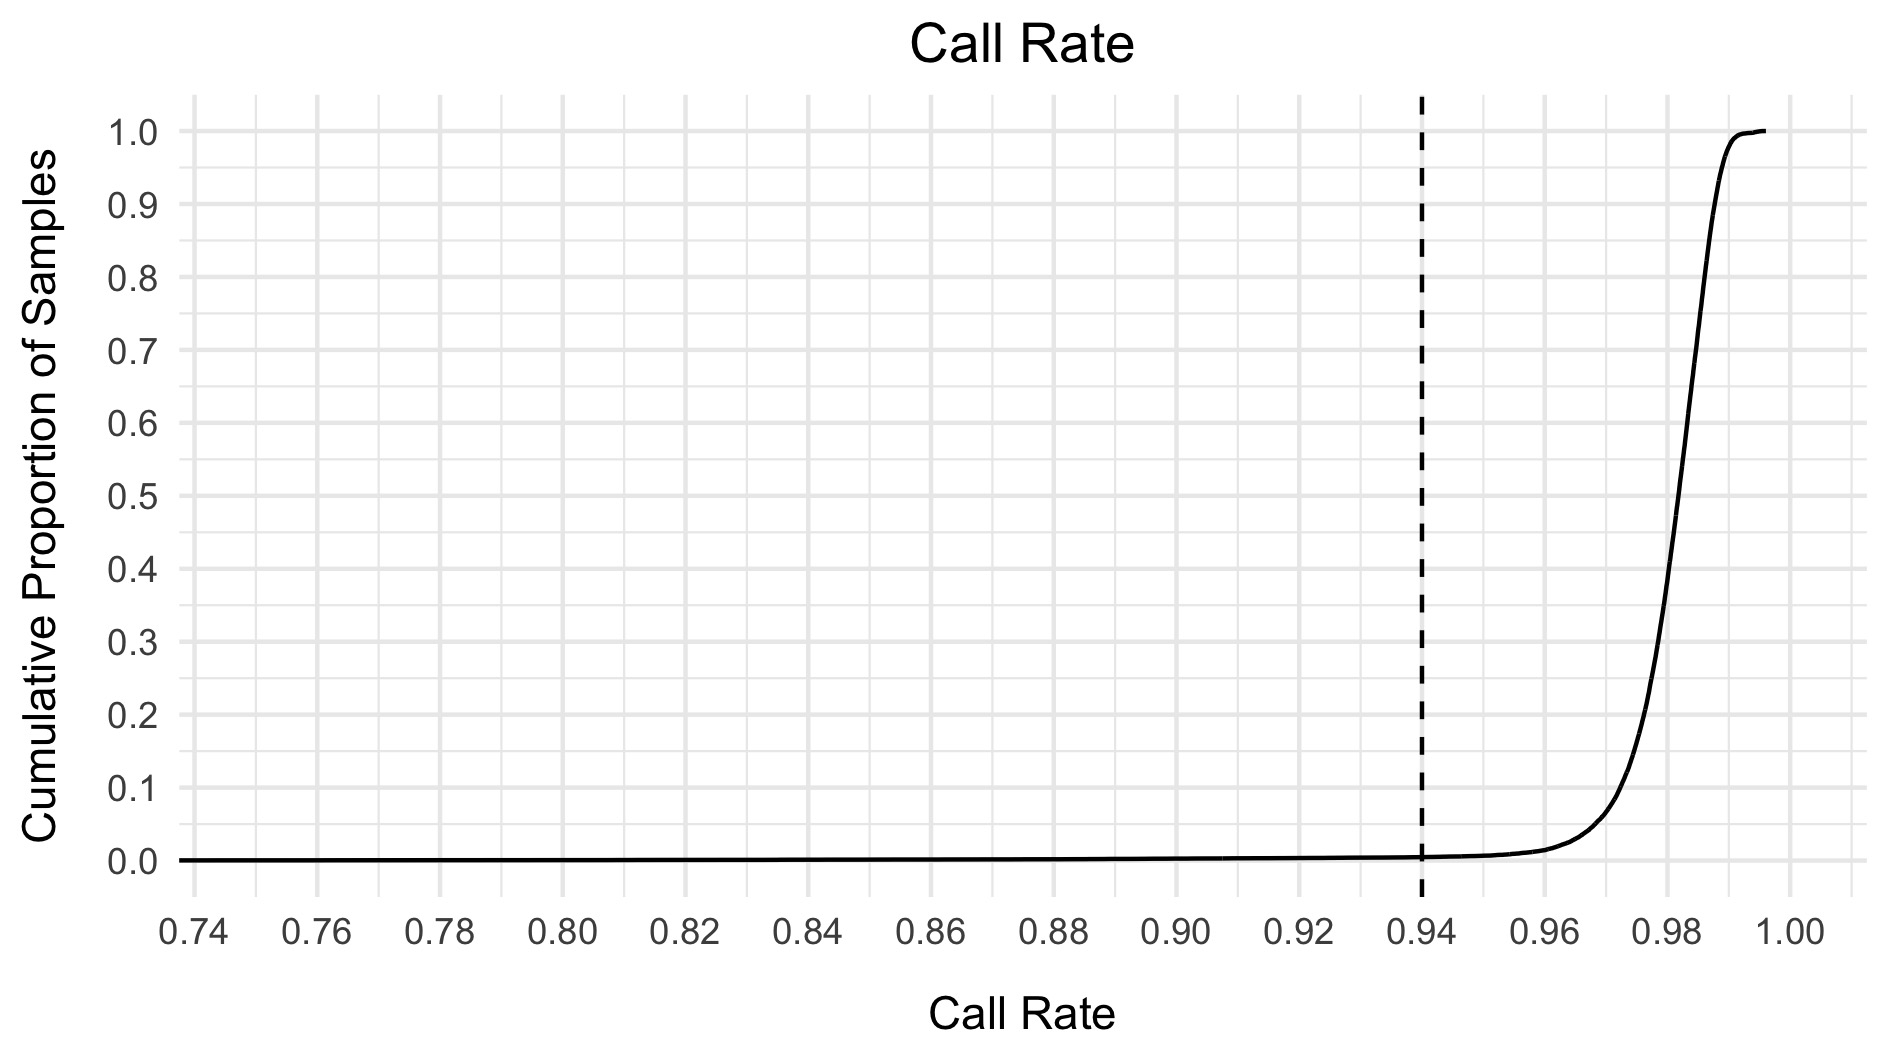
\includegraphics[width=0.5\textwidth]{03_callRate_cdf.jpg}}
\subfloat{\label{fig:contamination_cdf}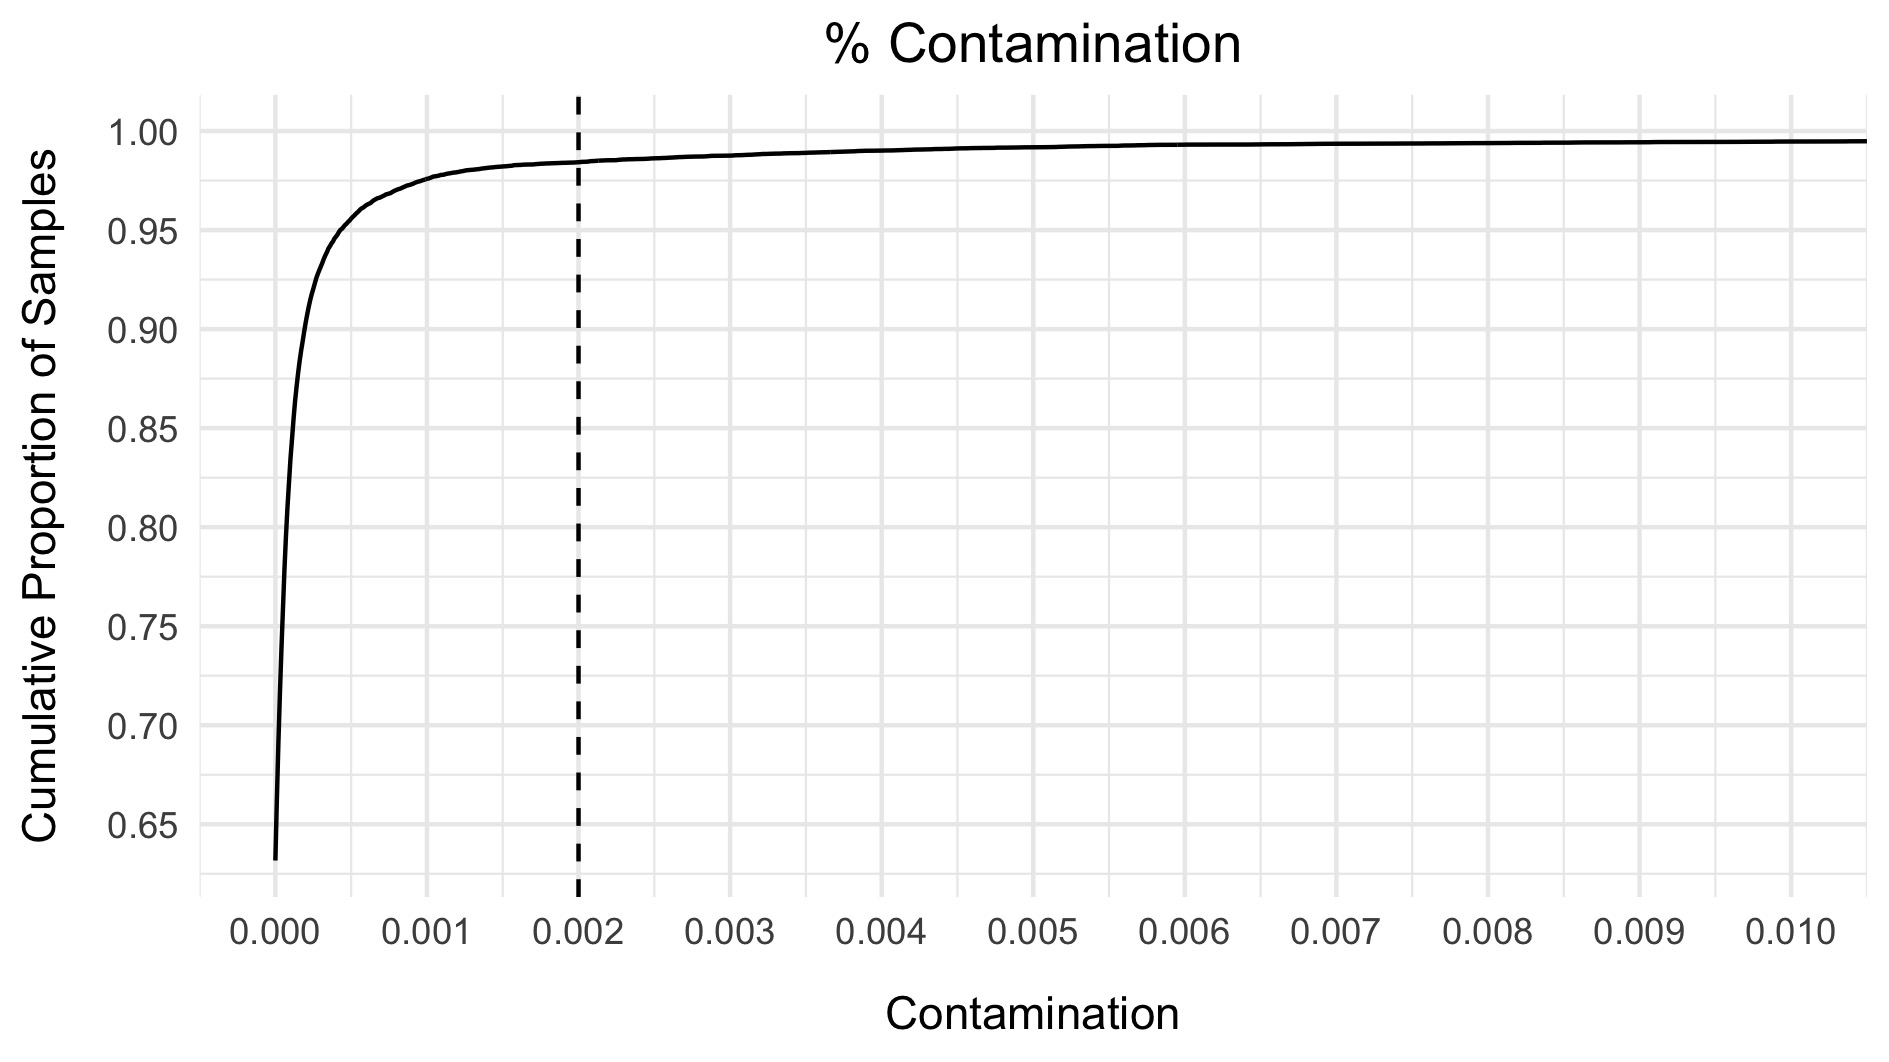
\includegraphics[width=0.5\textwidth]{03_contamination_cdf.jpg}}\\
\subfloat{\label{fig:chimeras_cdf}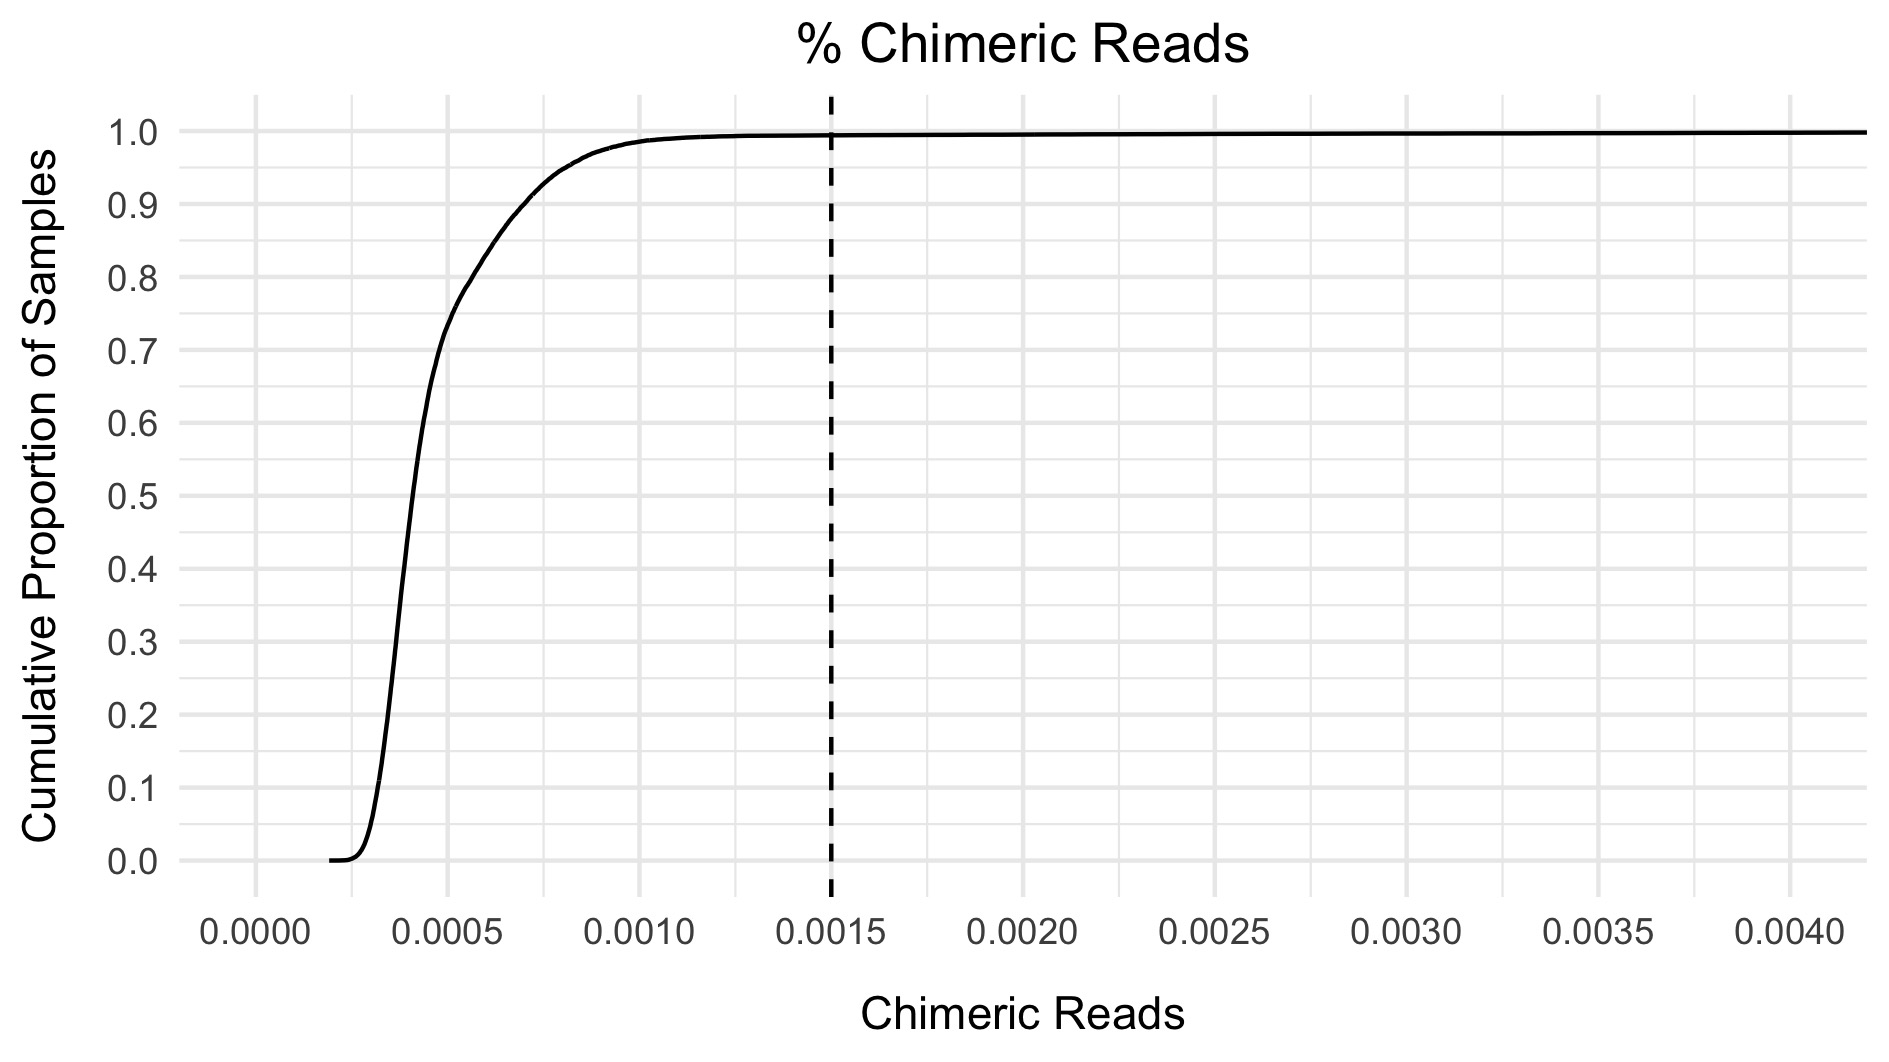
\includegraphics[width=0.5\textwidth]{03_chimeras_cdf.jpg}}
\subfloat{\label{fig:depth_cdf}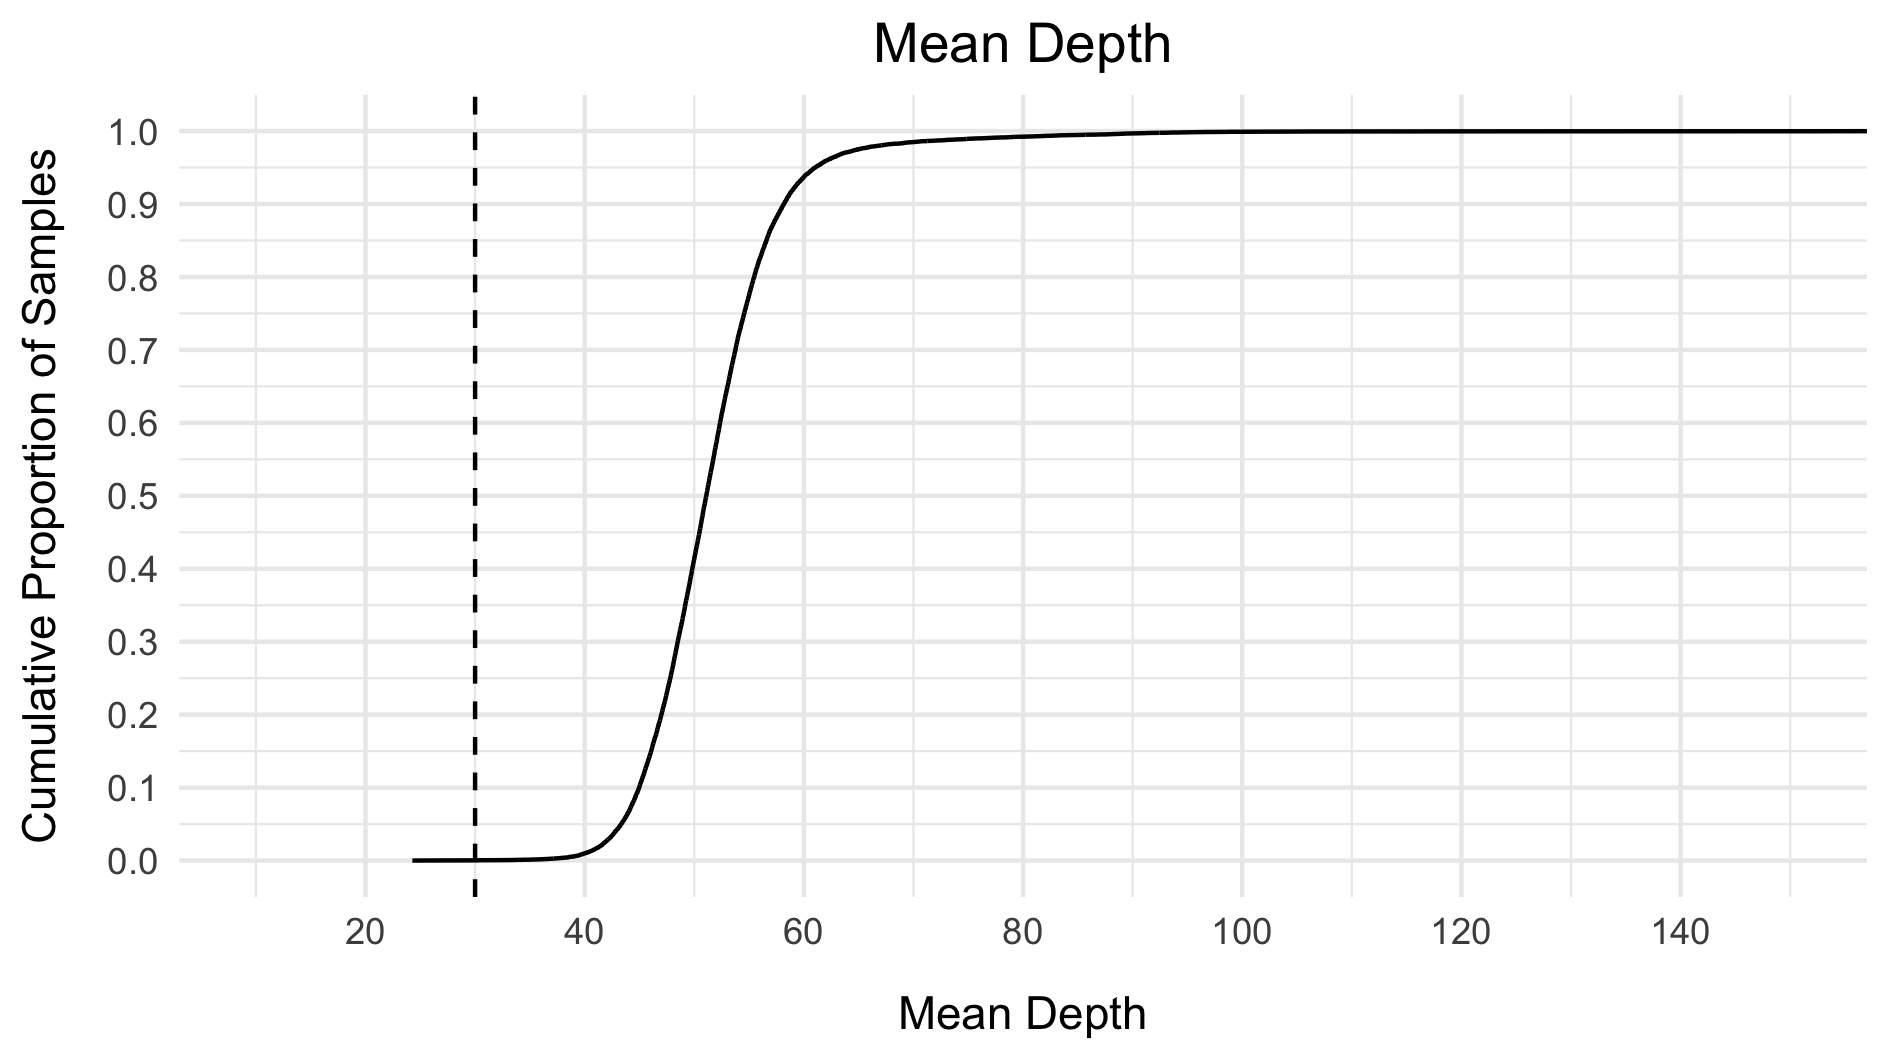
\includegraphics[width=0.5\textwidth]{03_dpMean_cdf.jpg}}\\
\subfloat{\label{fig:genotype_quality_cdf}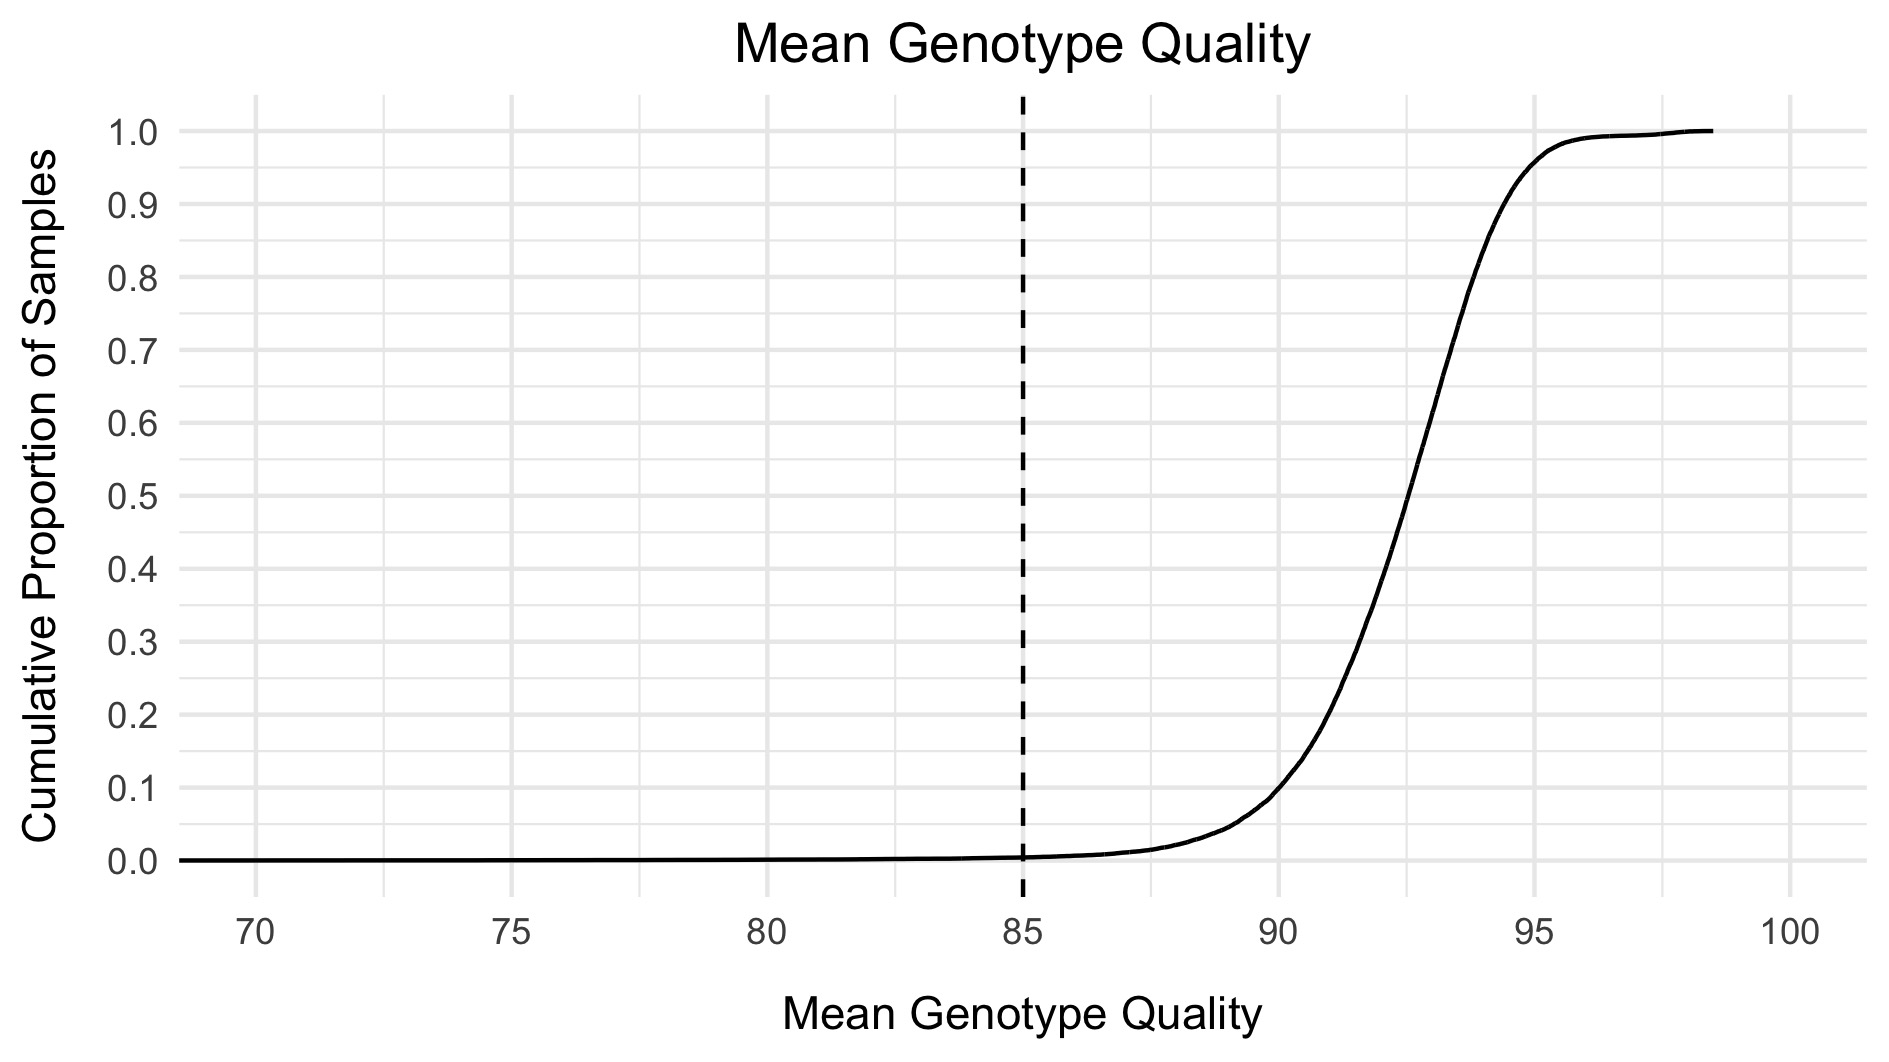
\includegraphics[width=0.5\textwidth]{03_gqMean_cdf.jpg}}
\caption{CDFs of various metrics of sample quality with thresholds for inclusion/exclusion.}
\label{fig:initial_sample_qc}
\end{figure}

% IMPUTE SEX.
\begin{figure}
\centering
\subfloat{\label{fig:impute_sex_hist}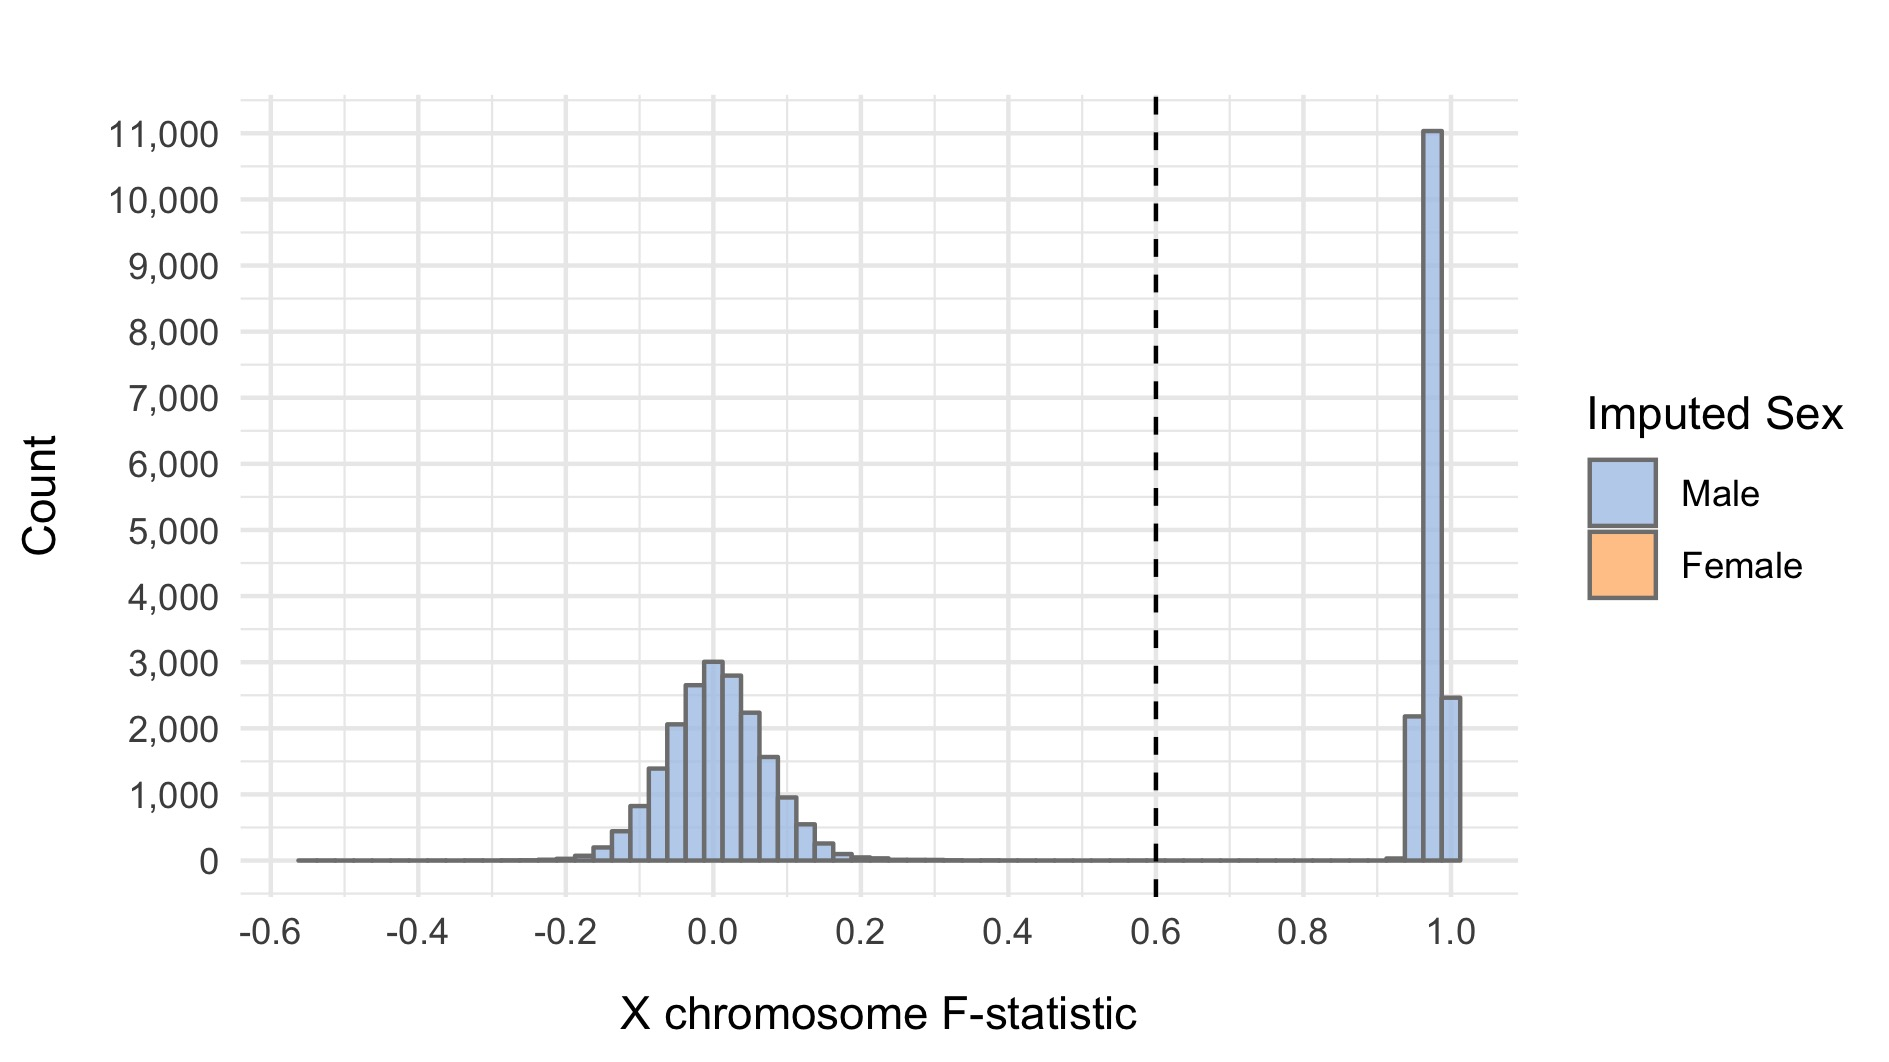
\includegraphics[width=0.5\textwidth]{05_imputesex_histogram.jpg}}
\subfloat{\label{fig:impute_sex_scatter_box}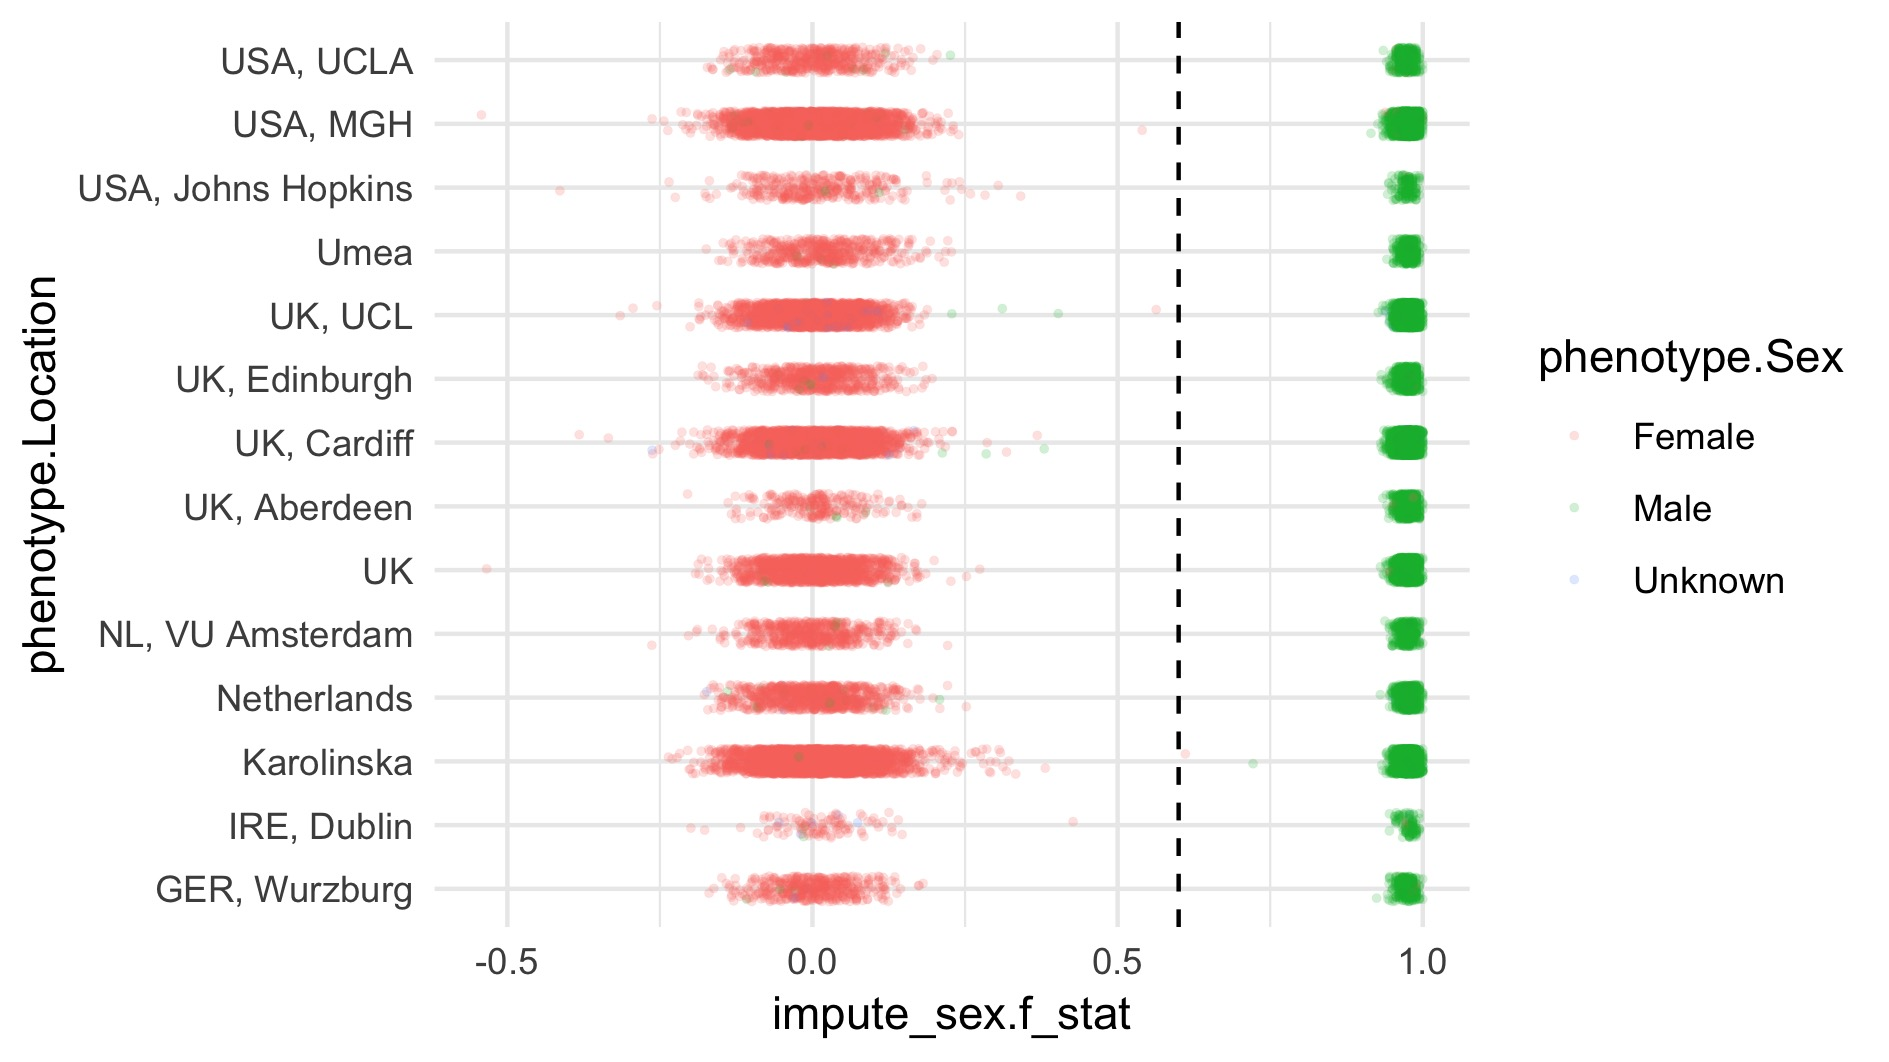
\includegraphics[width=0.5\textwidth]{05_imputesex_scatter_box.jpg}}\\
\subfloat{\label{fig:impute_sex_scatter}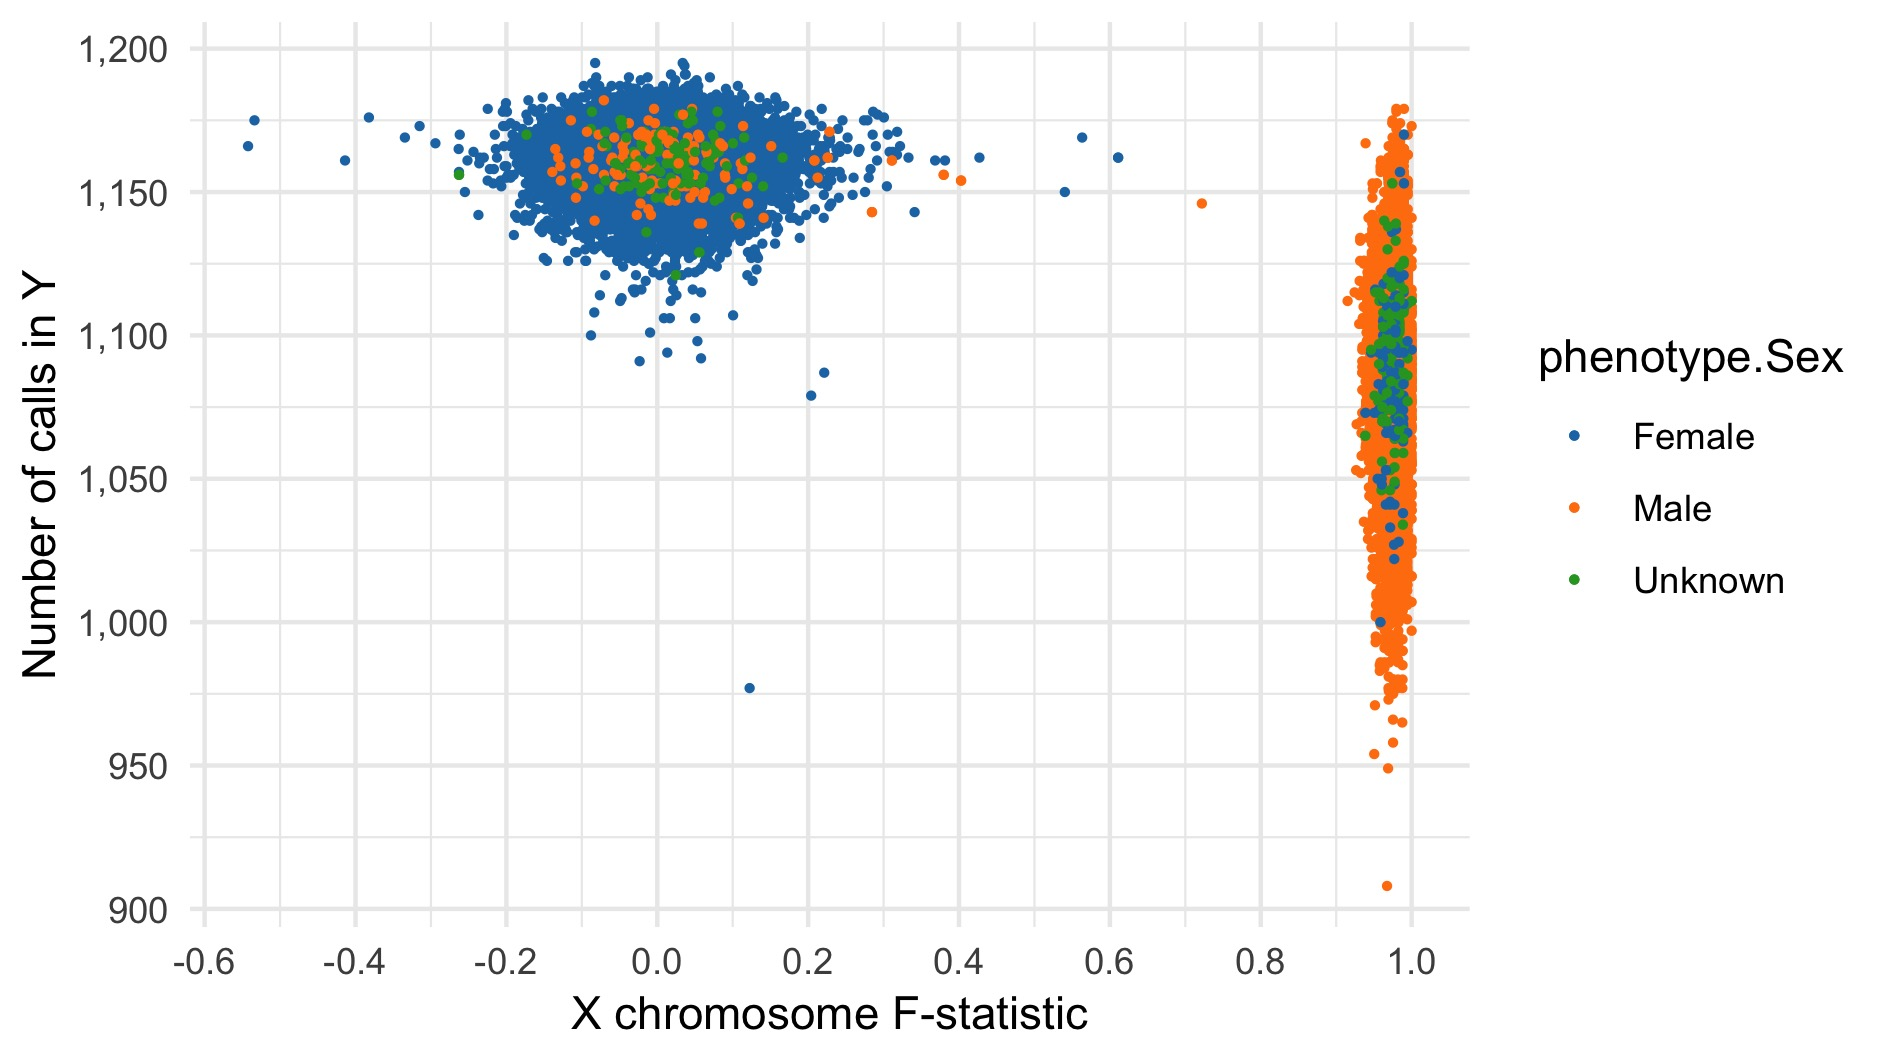
\includegraphics[width=0.8\textwidth]{05_imputesex_scatter.jpg}}
\caption{F-statistic used to determine if individual is male or female. Threshold set at 0.6.}
\label{fig:impute_sex}
\end{figure}

% IBD FILTER.
\begin{figure}
\centering
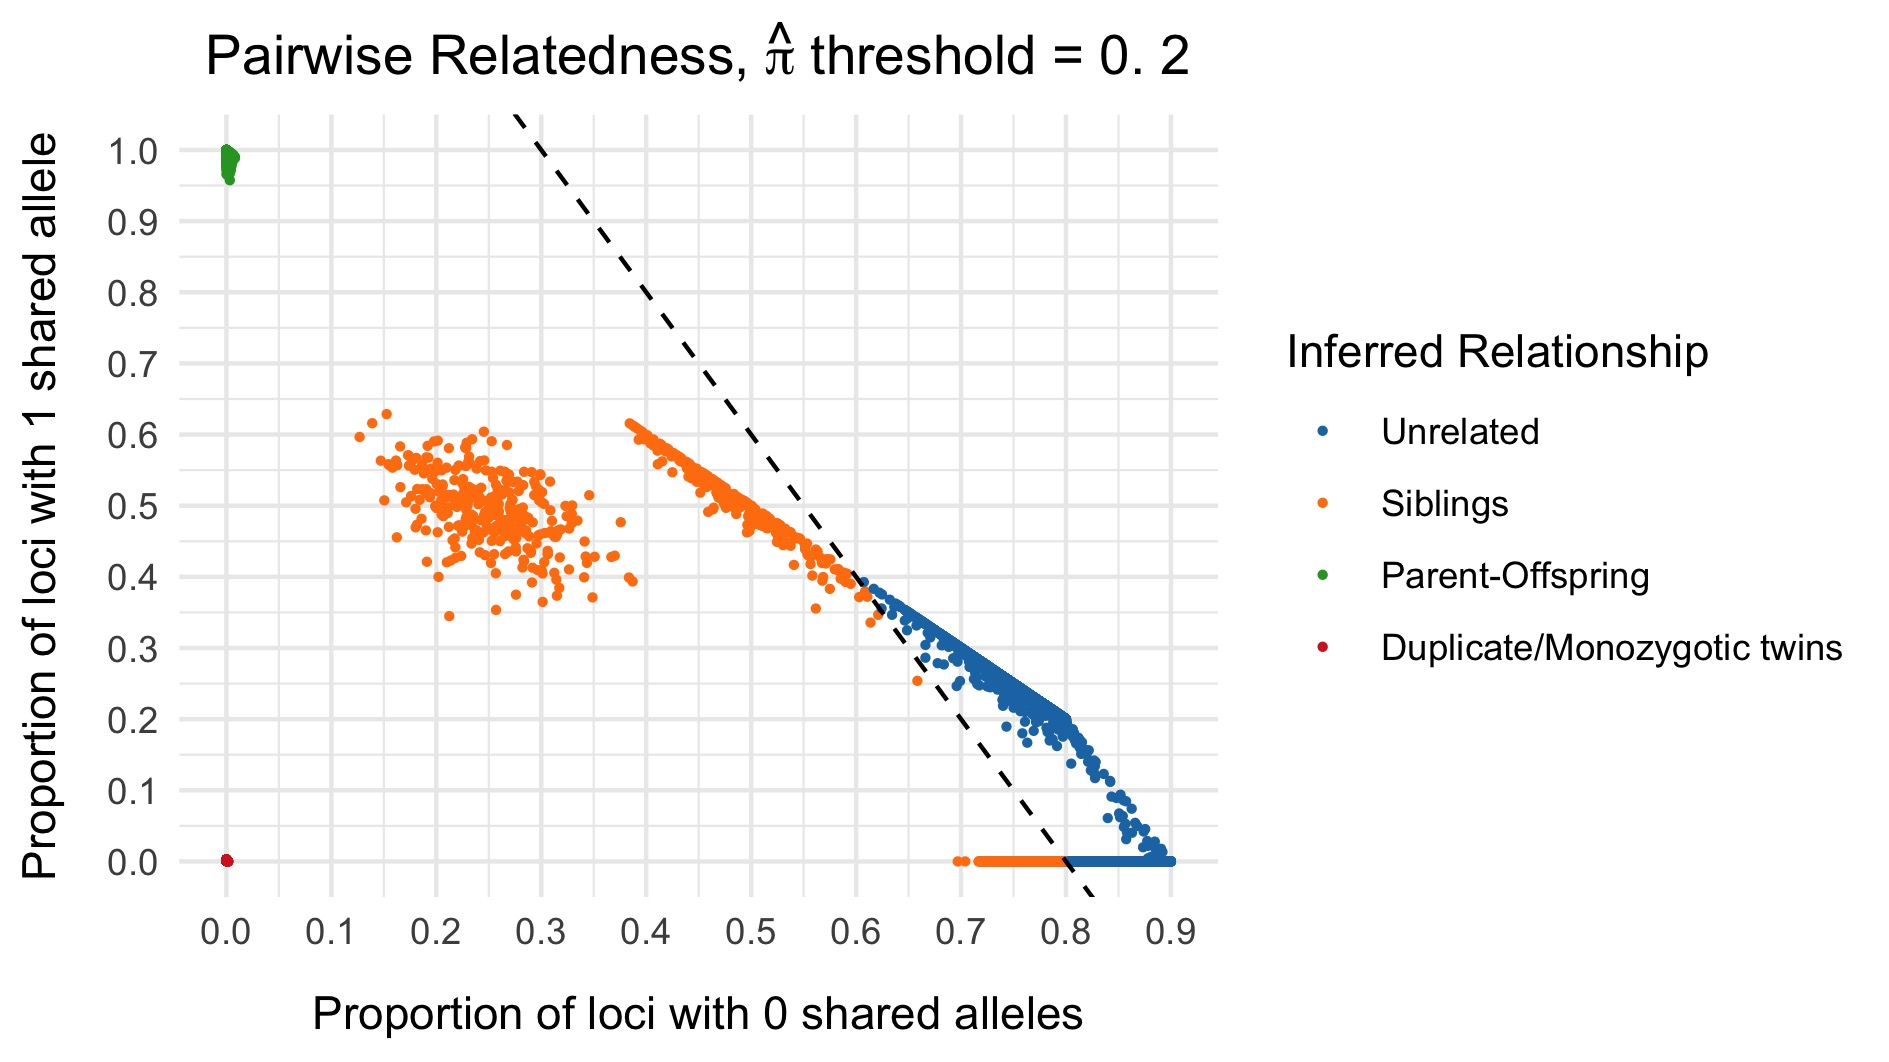
\includegraphics[width=0.7\textwidth]{06_IBD_plot.jpg}
\caption{IBD plot. Threshold for `related' set at $\hat{\pi} > 0.2$.}
\label{fig:IBD_plot}
\end{figure}

% PCA.
\begin{figure}
\centering
\subfloat{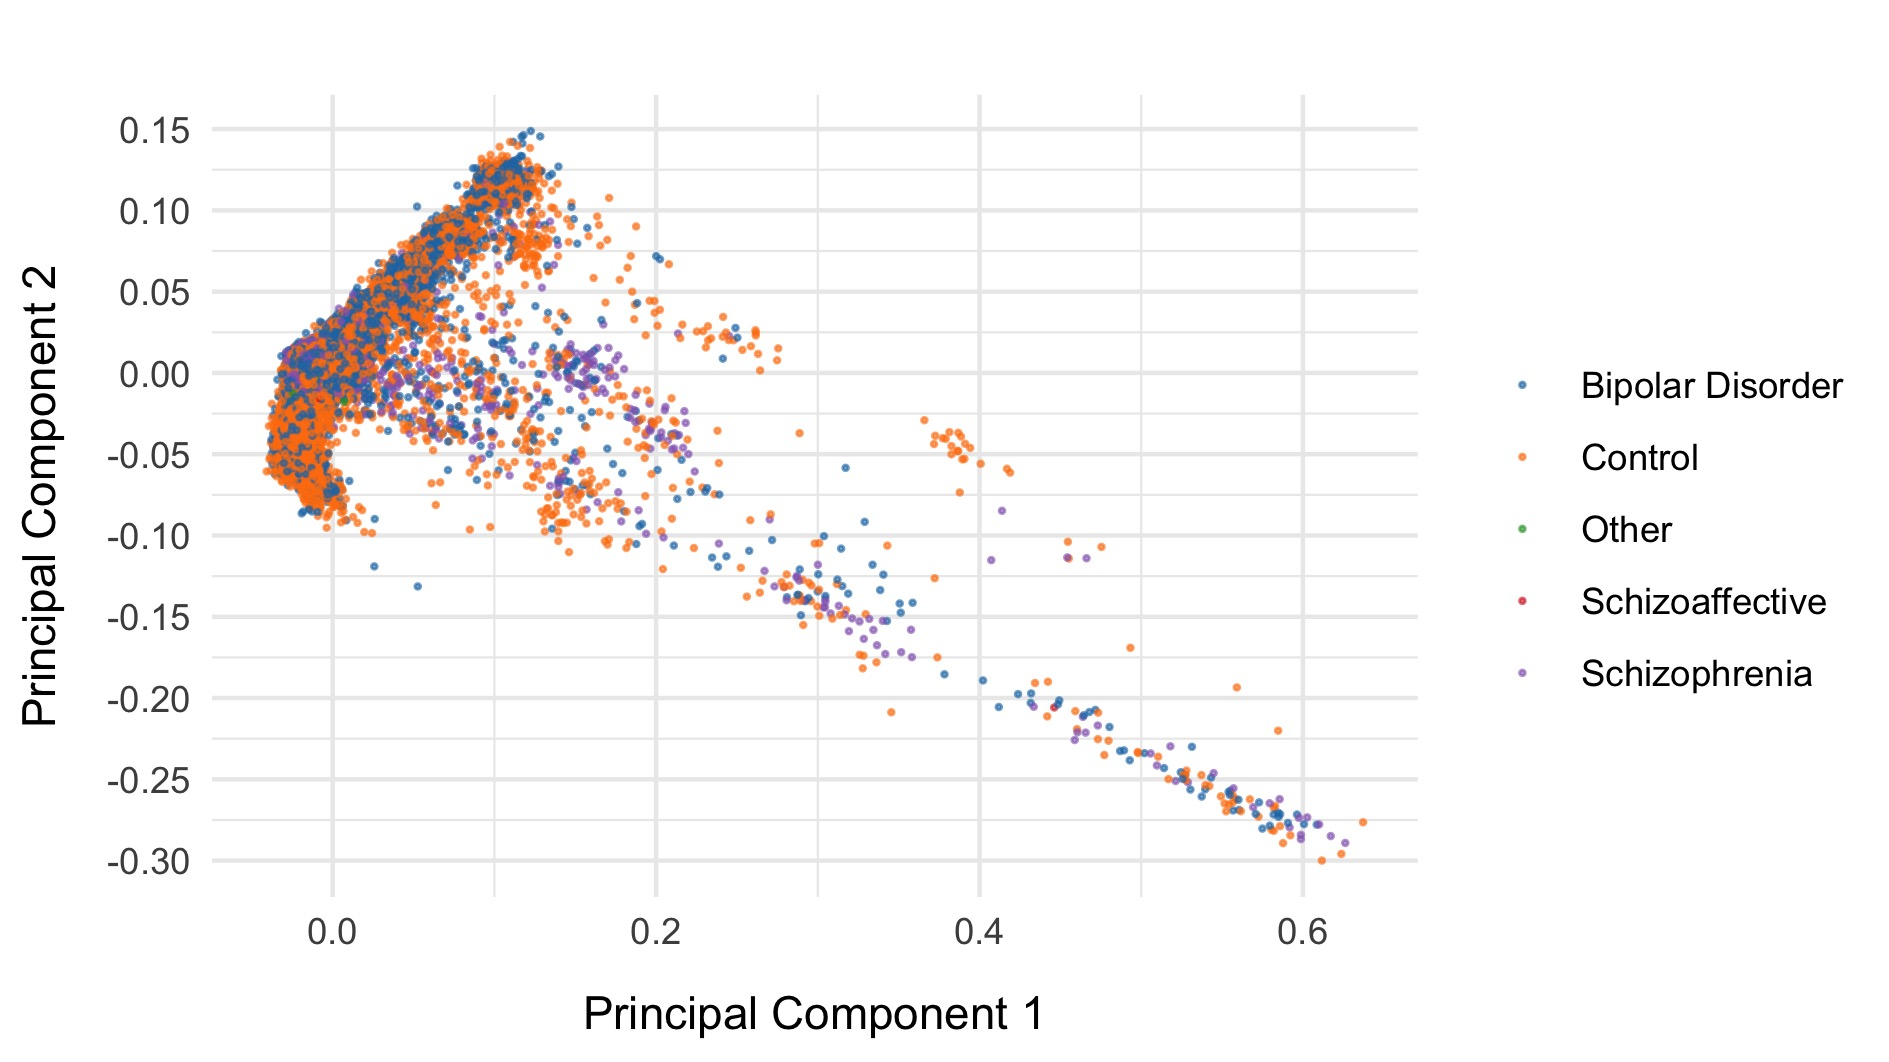
\includegraphics[width=0.5\textwidth]{09_PC1_PC2.jpg}}
\subfloat{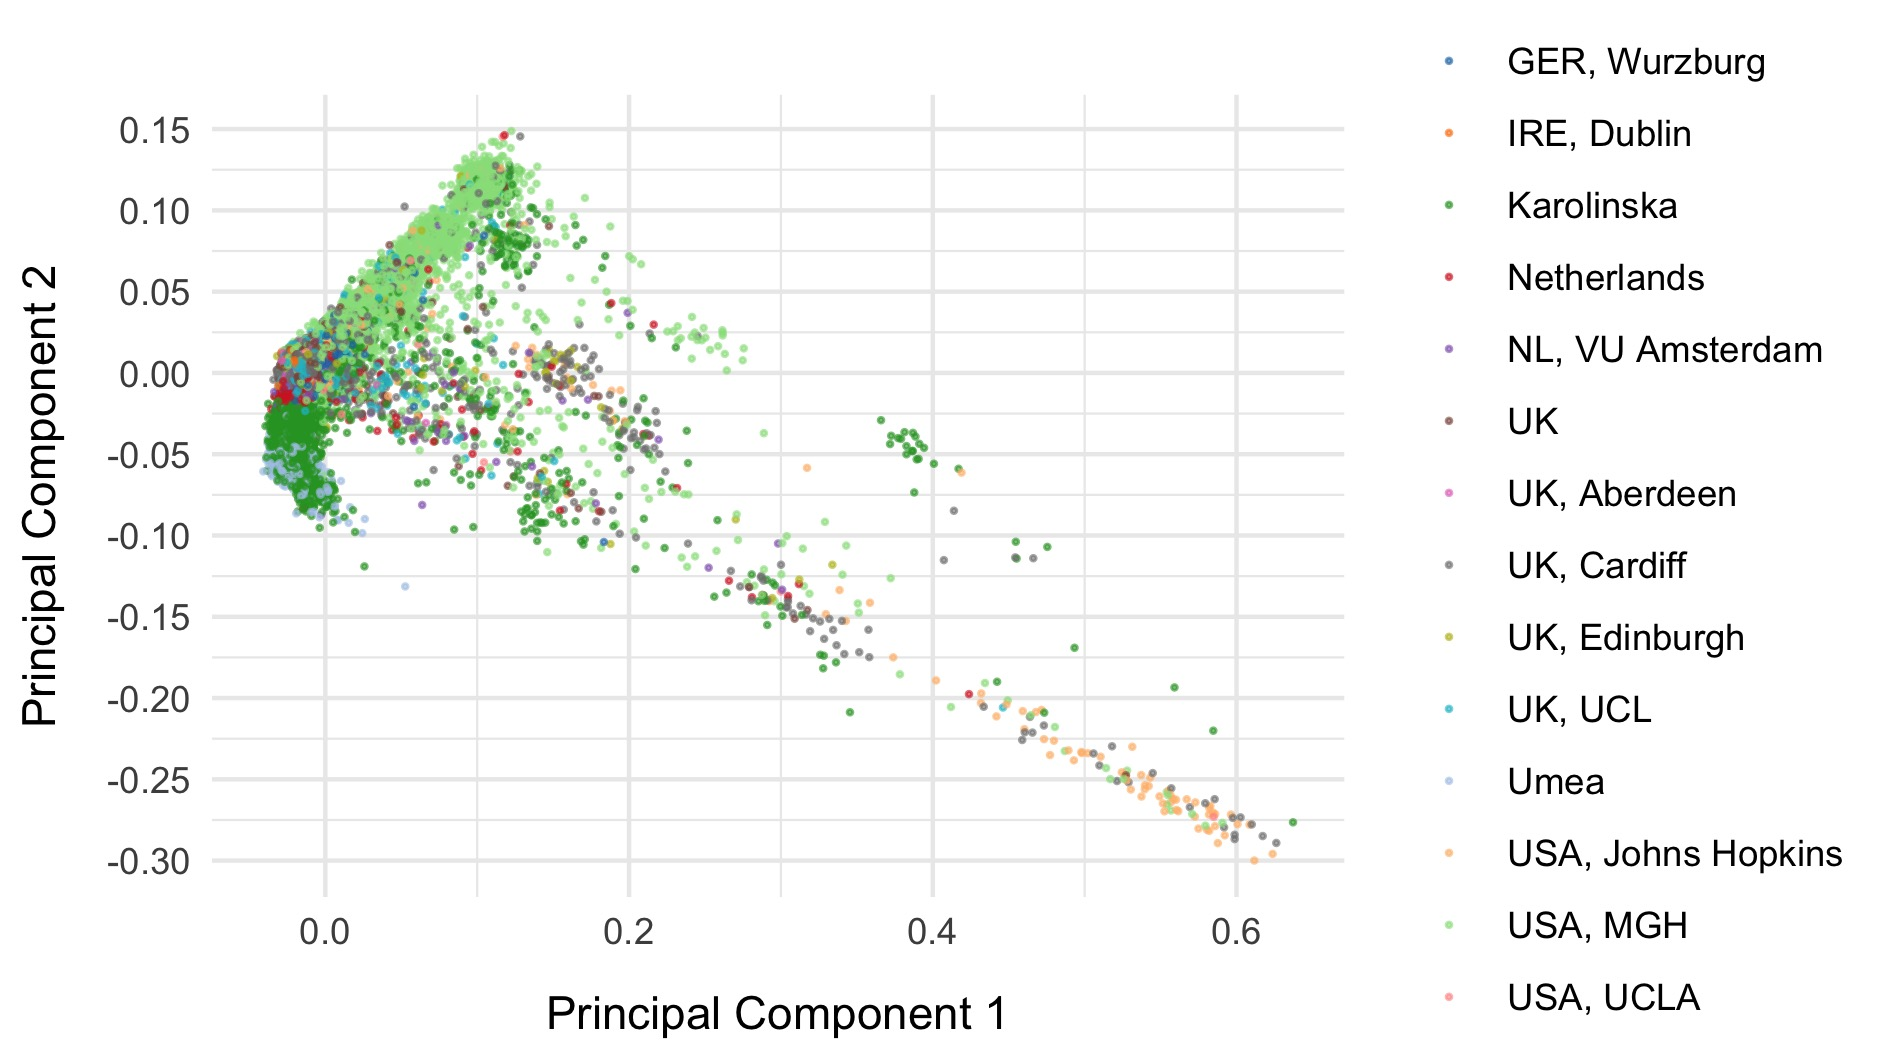
\includegraphics[width=0.5\textwidth]{09_PC1_PC2_collection.jpg}}\\
\subfloat{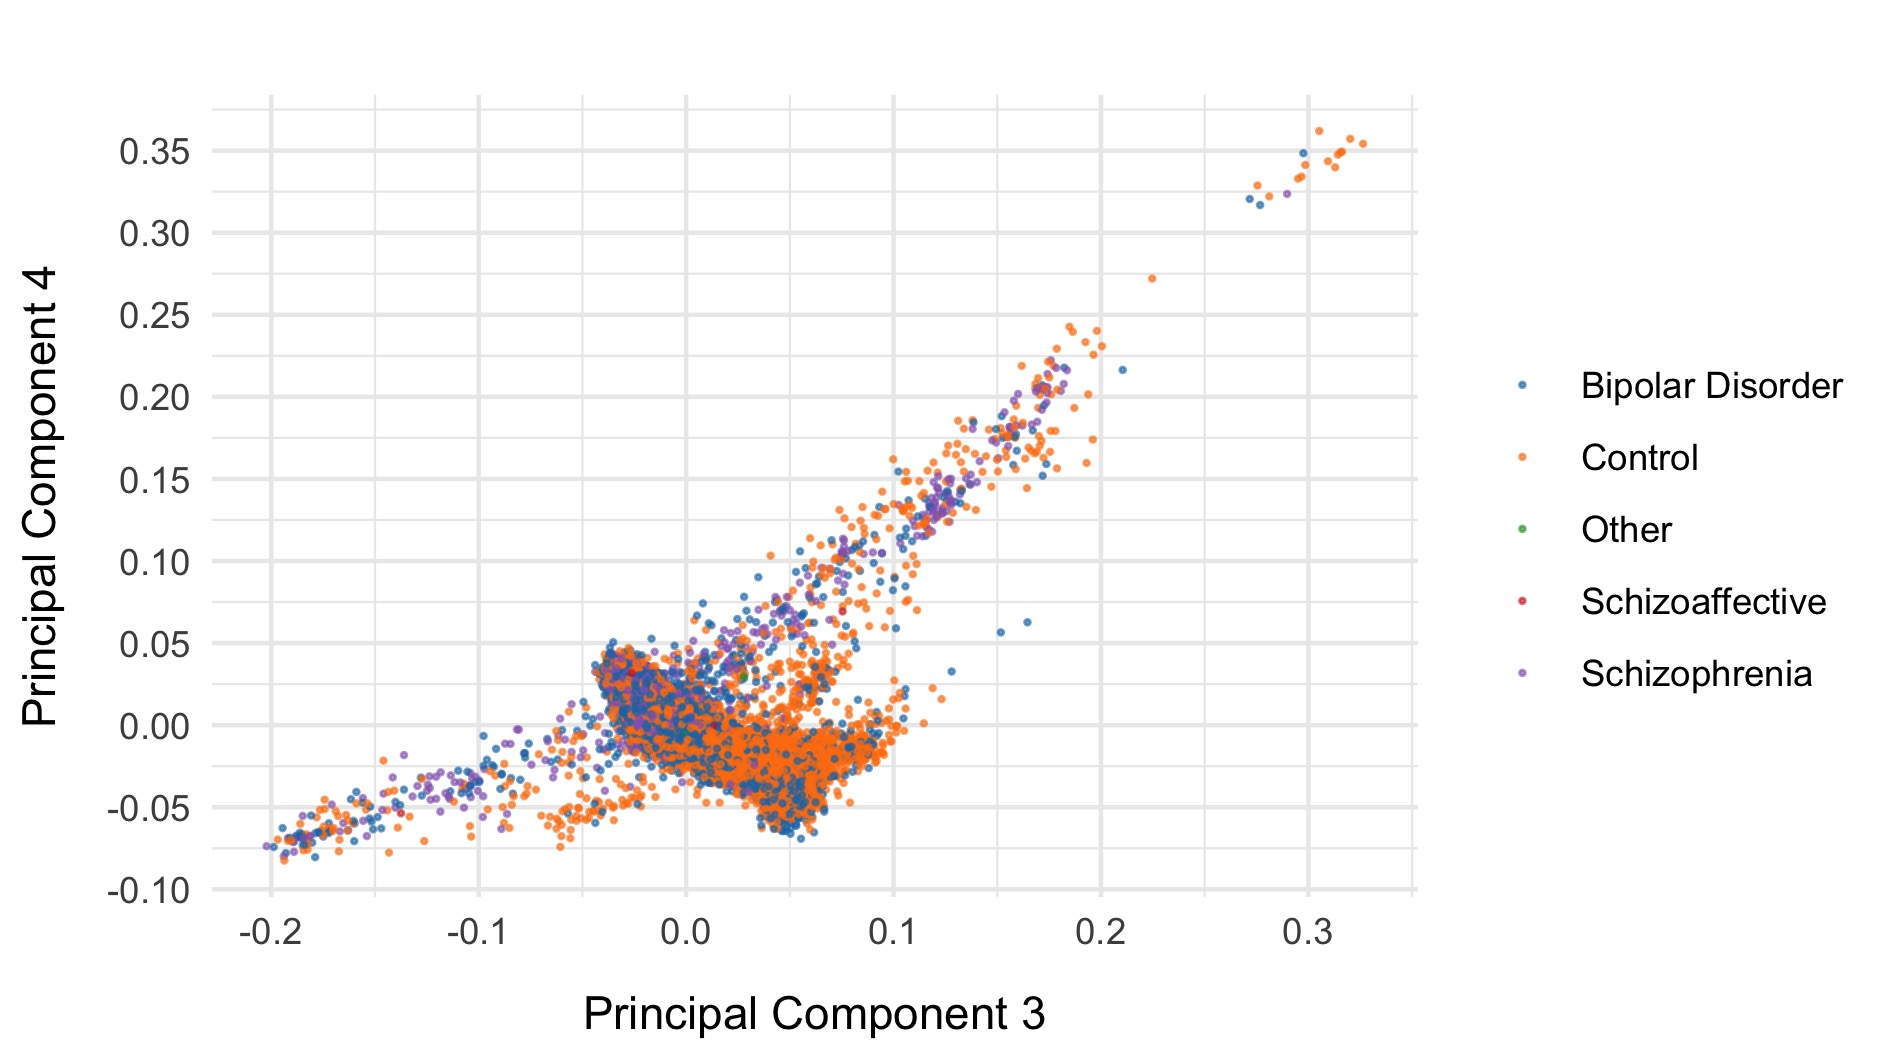
\includegraphics[width=0.5\textwidth]{09_PC3_PC4.jpg}}
\subfloat{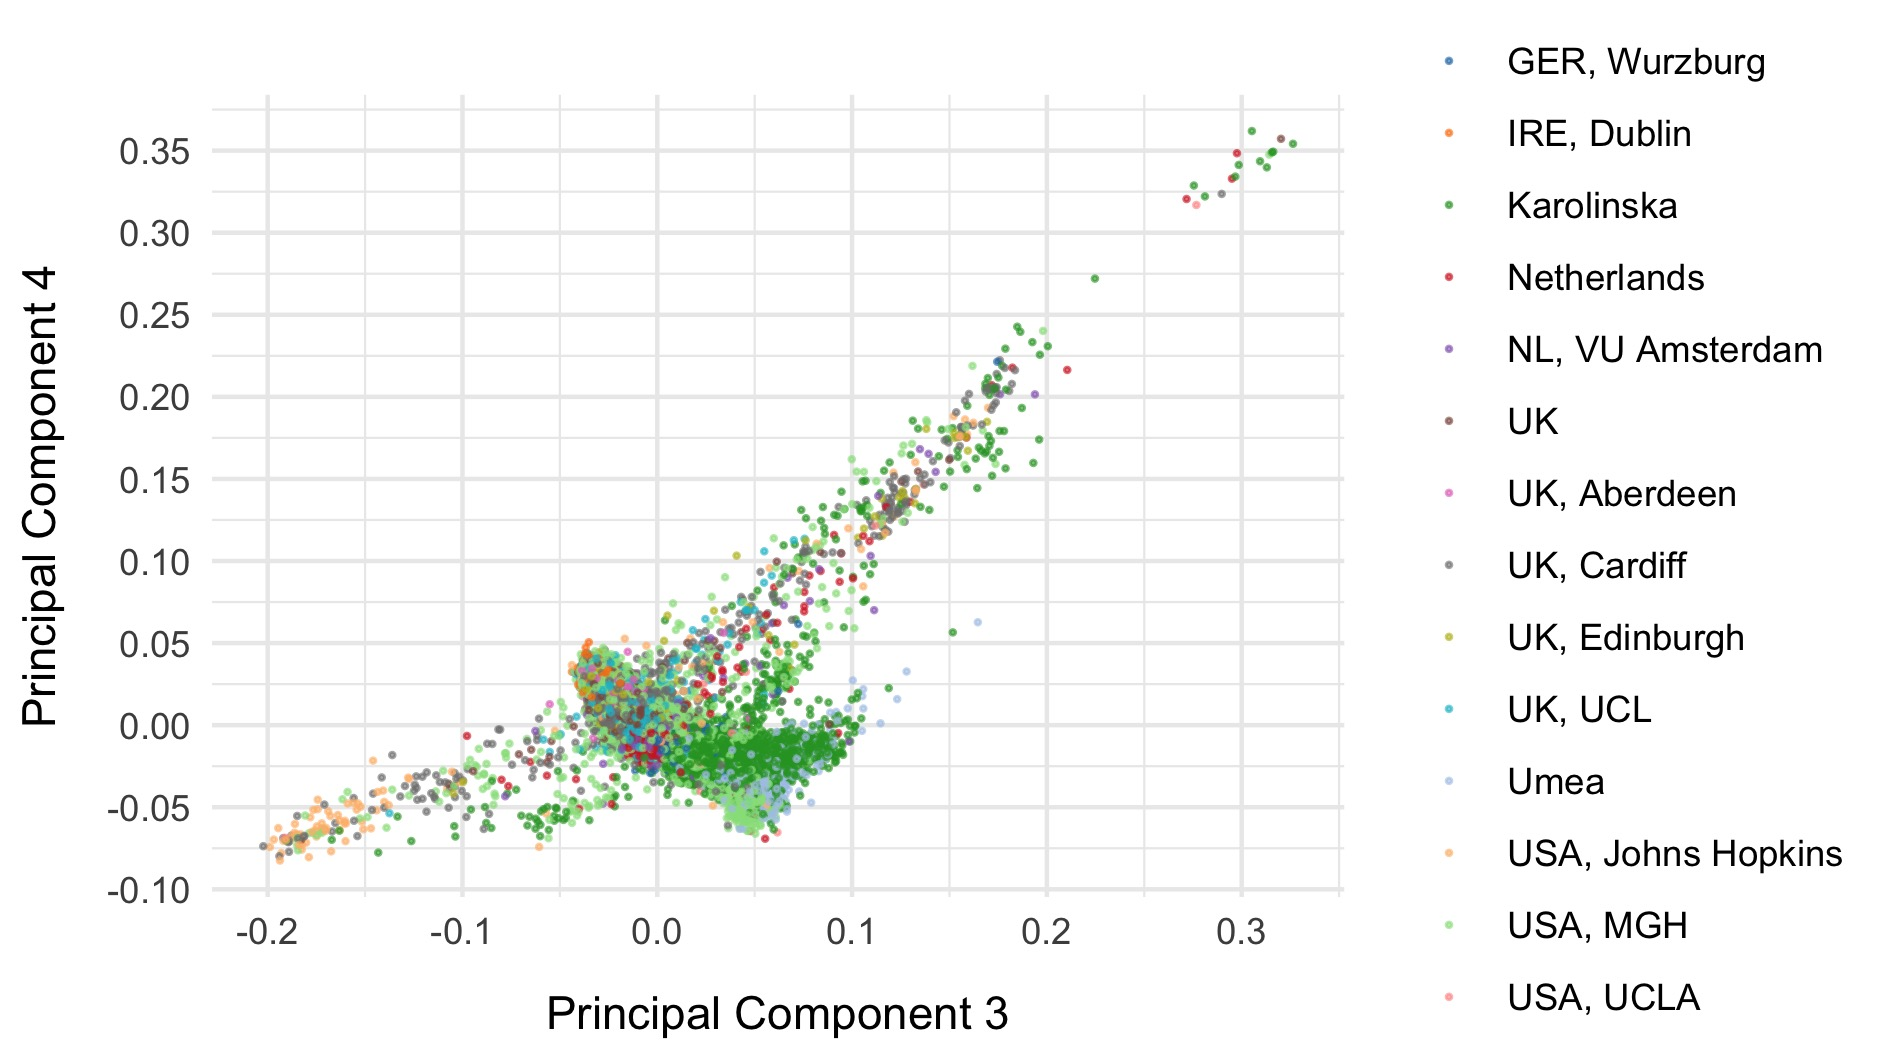
\includegraphics[width=0.5\textwidth]{09_PC3_PC4_collection.jpg}}\\
\subfloat{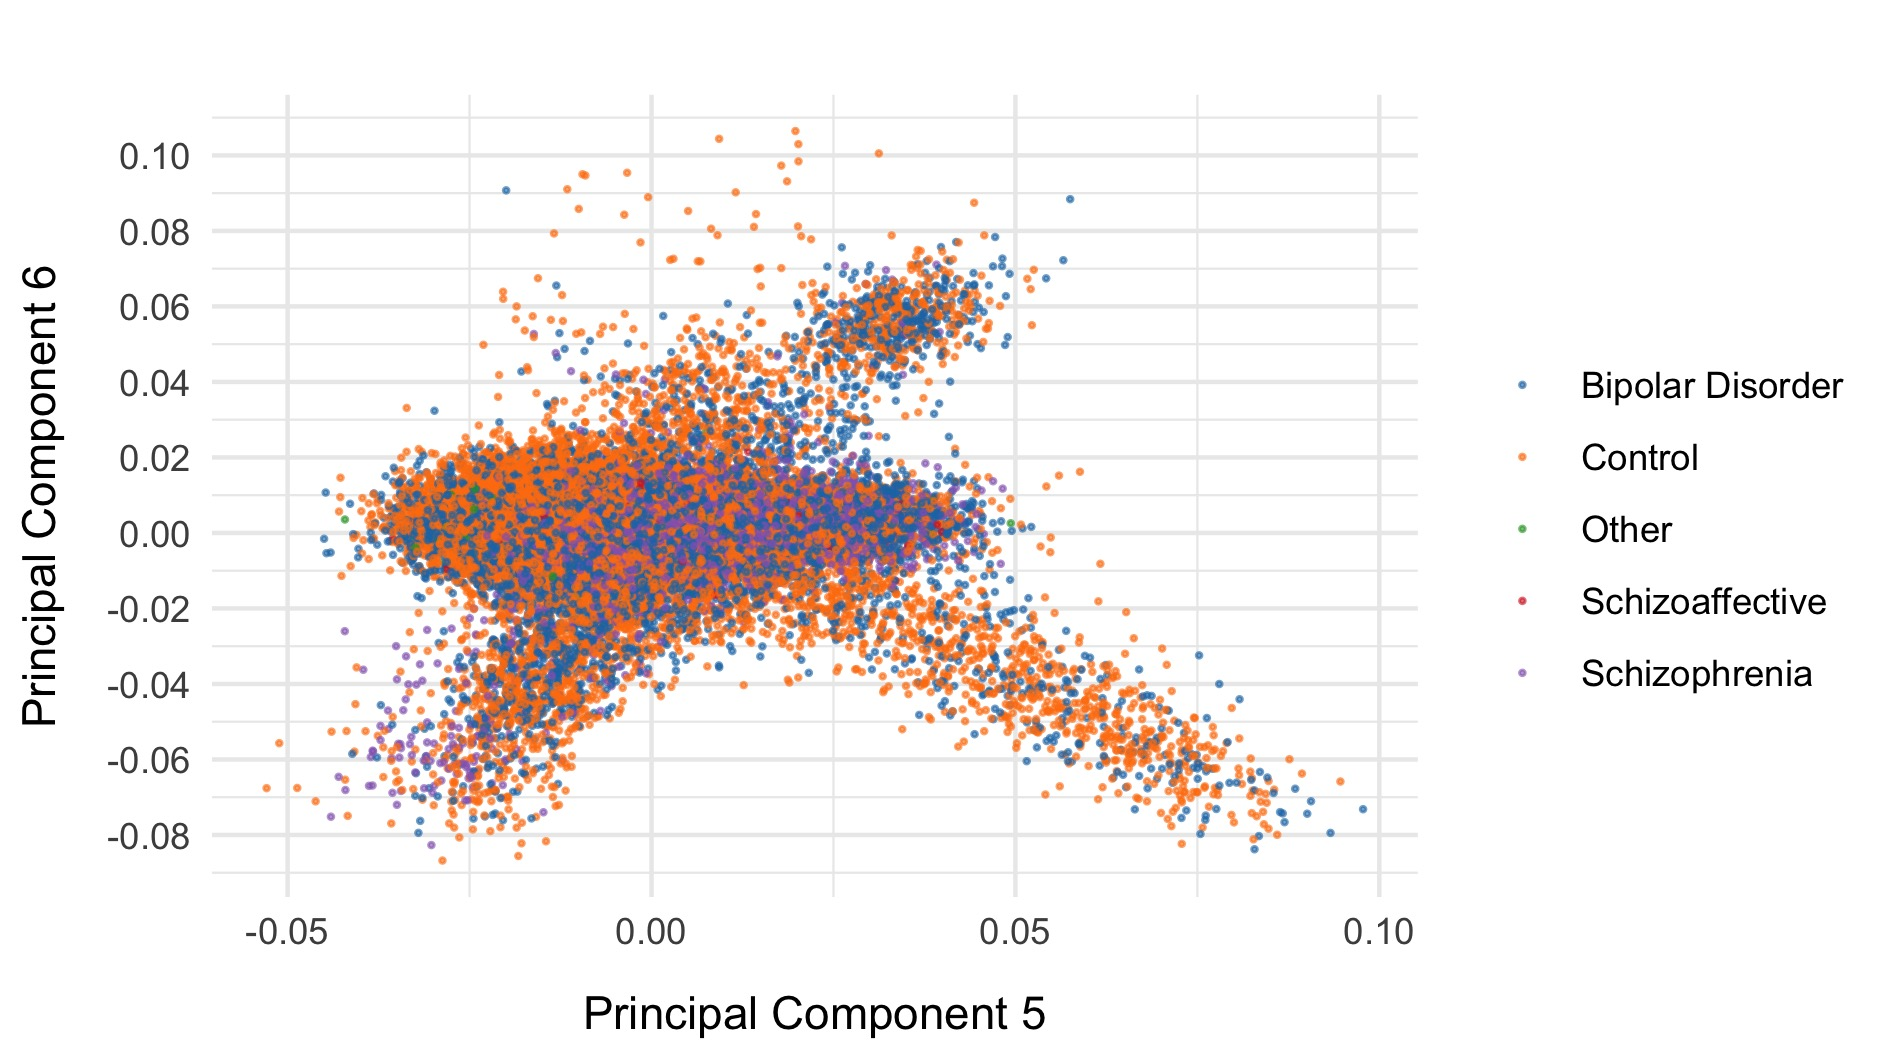
\includegraphics[width=0.5\textwidth]{09_PC5_PC6.jpg}}
\subfloat{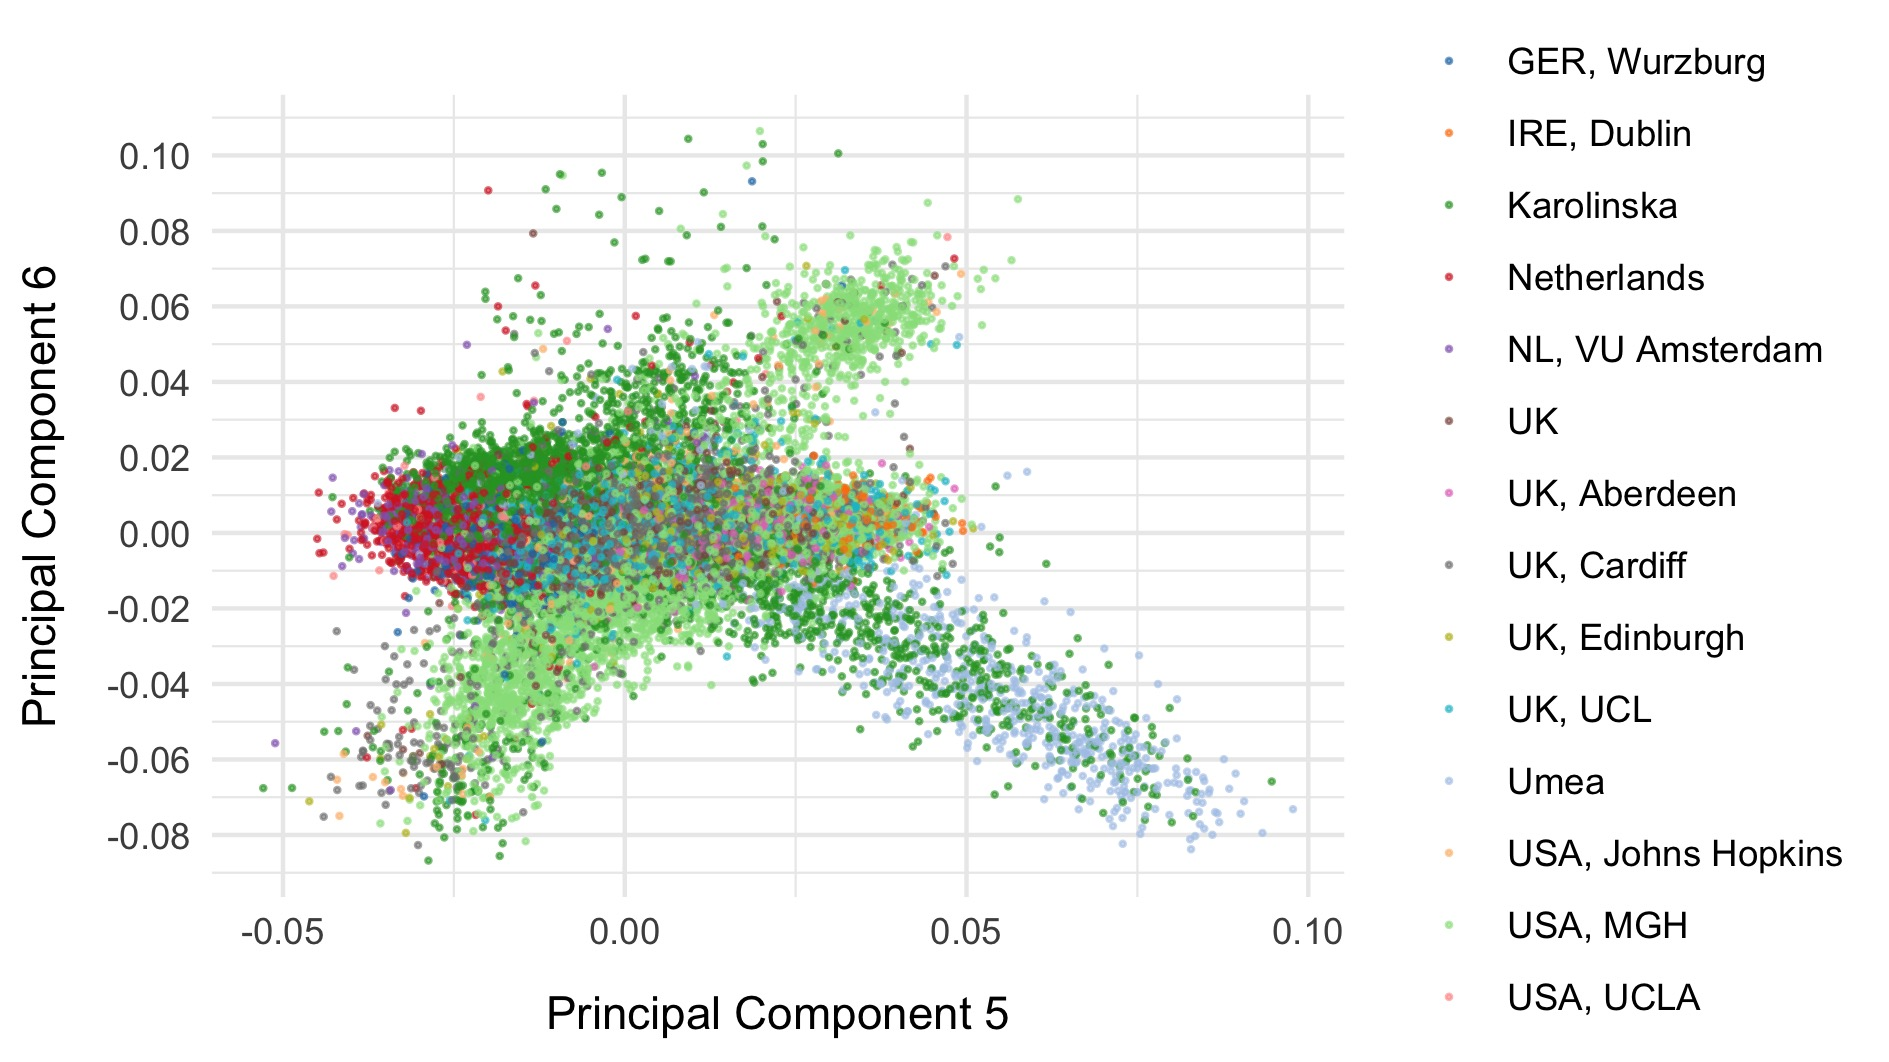
\includegraphics[width=0.5\textwidth]{09_PC5_PC6_collection.jpg}}
\caption{Initial PCA of all samples}
\label{fig:PCA}
\end{figure}

% PCA with 1kg.
\begin{figure}
\centering
\subfloat{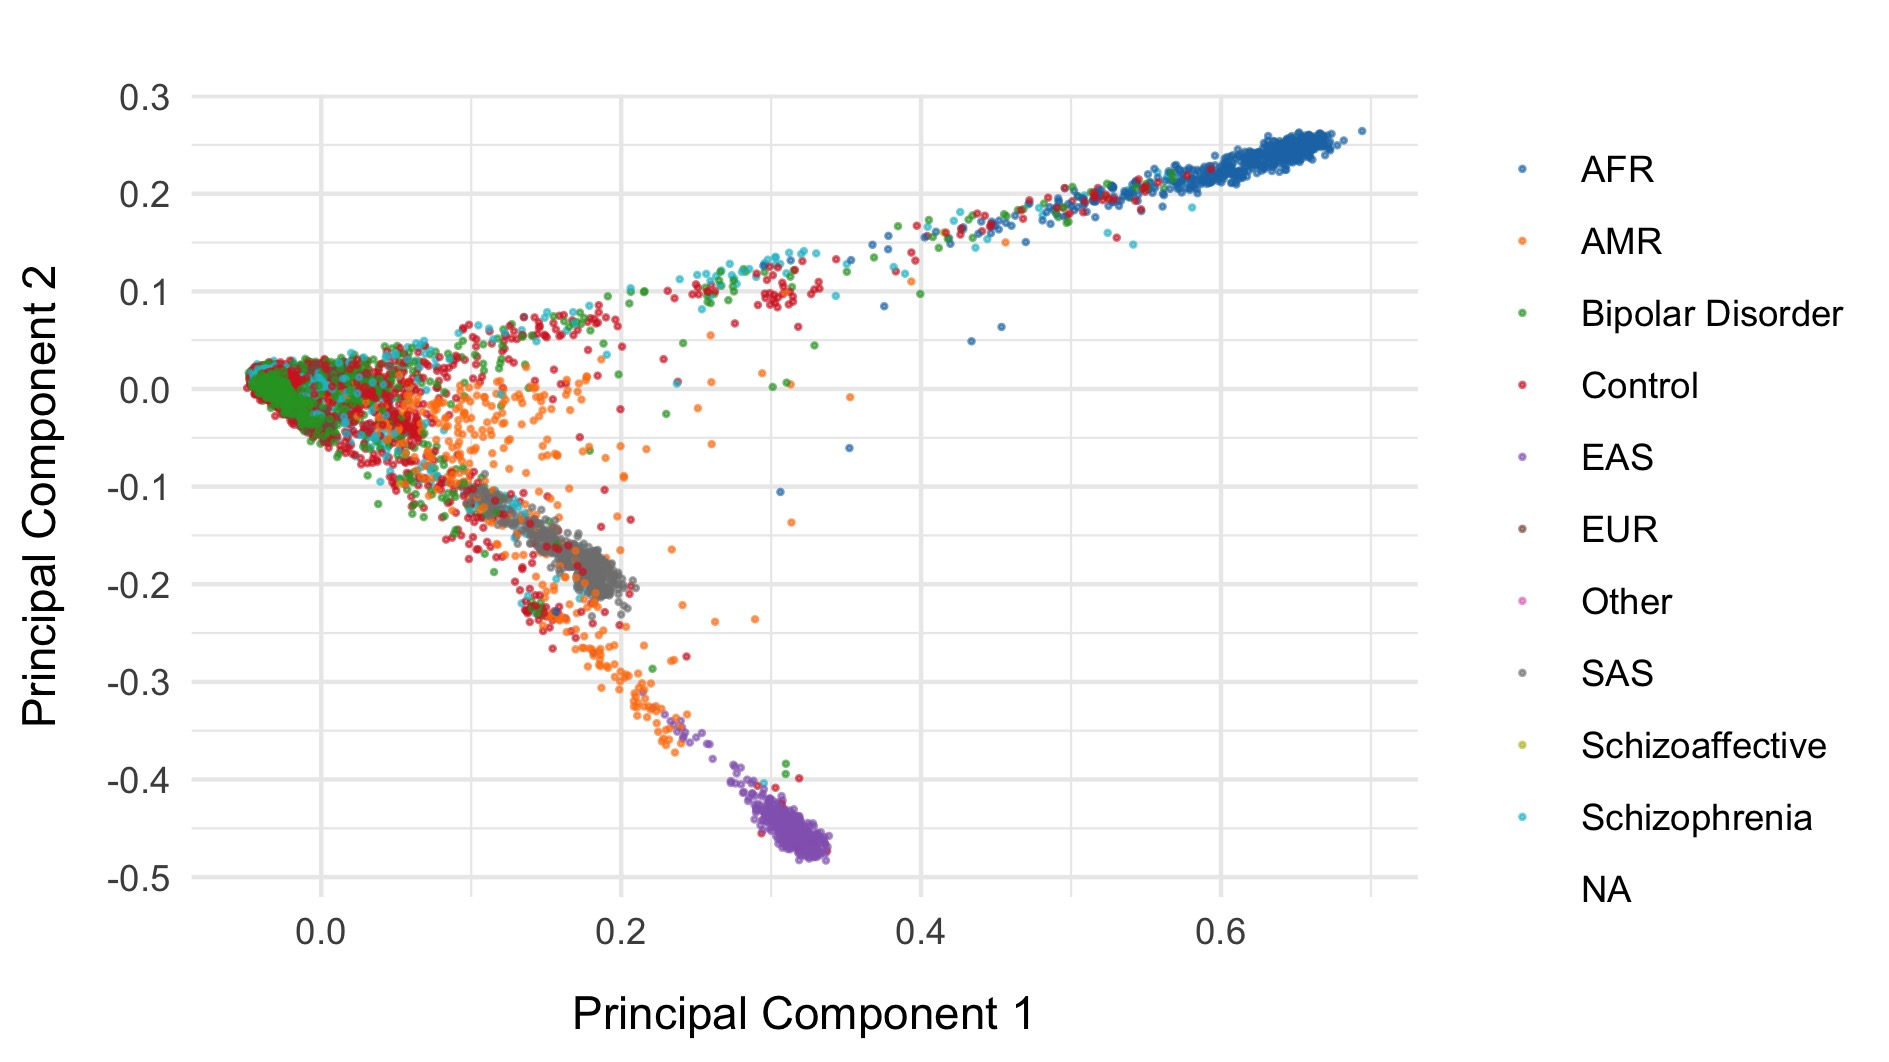
\includegraphics[width=0.5\textwidth]{10_PC1_PC2_1kg.jpg}}
\subfloat{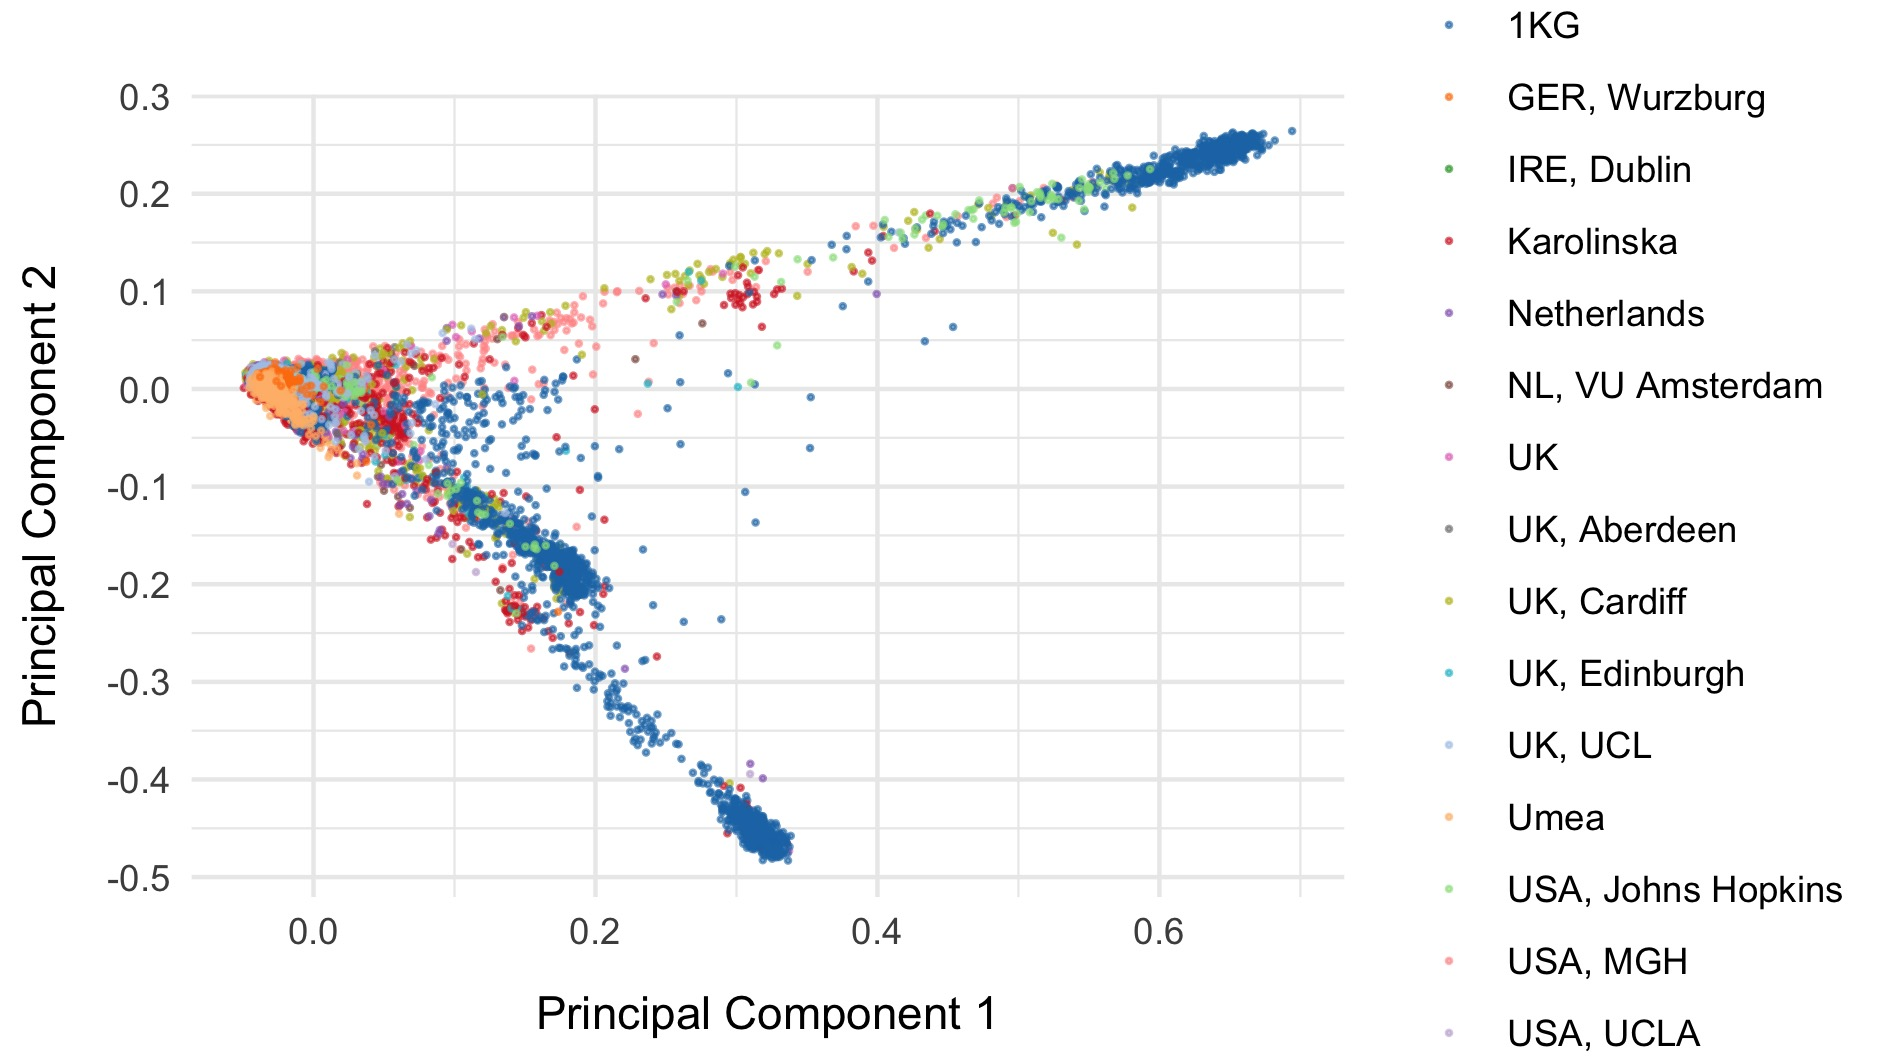
\includegraphics[width=0.5\textwidth]{10_PC1_PC2_1kg_collection.jpg}}\\
\subfloat{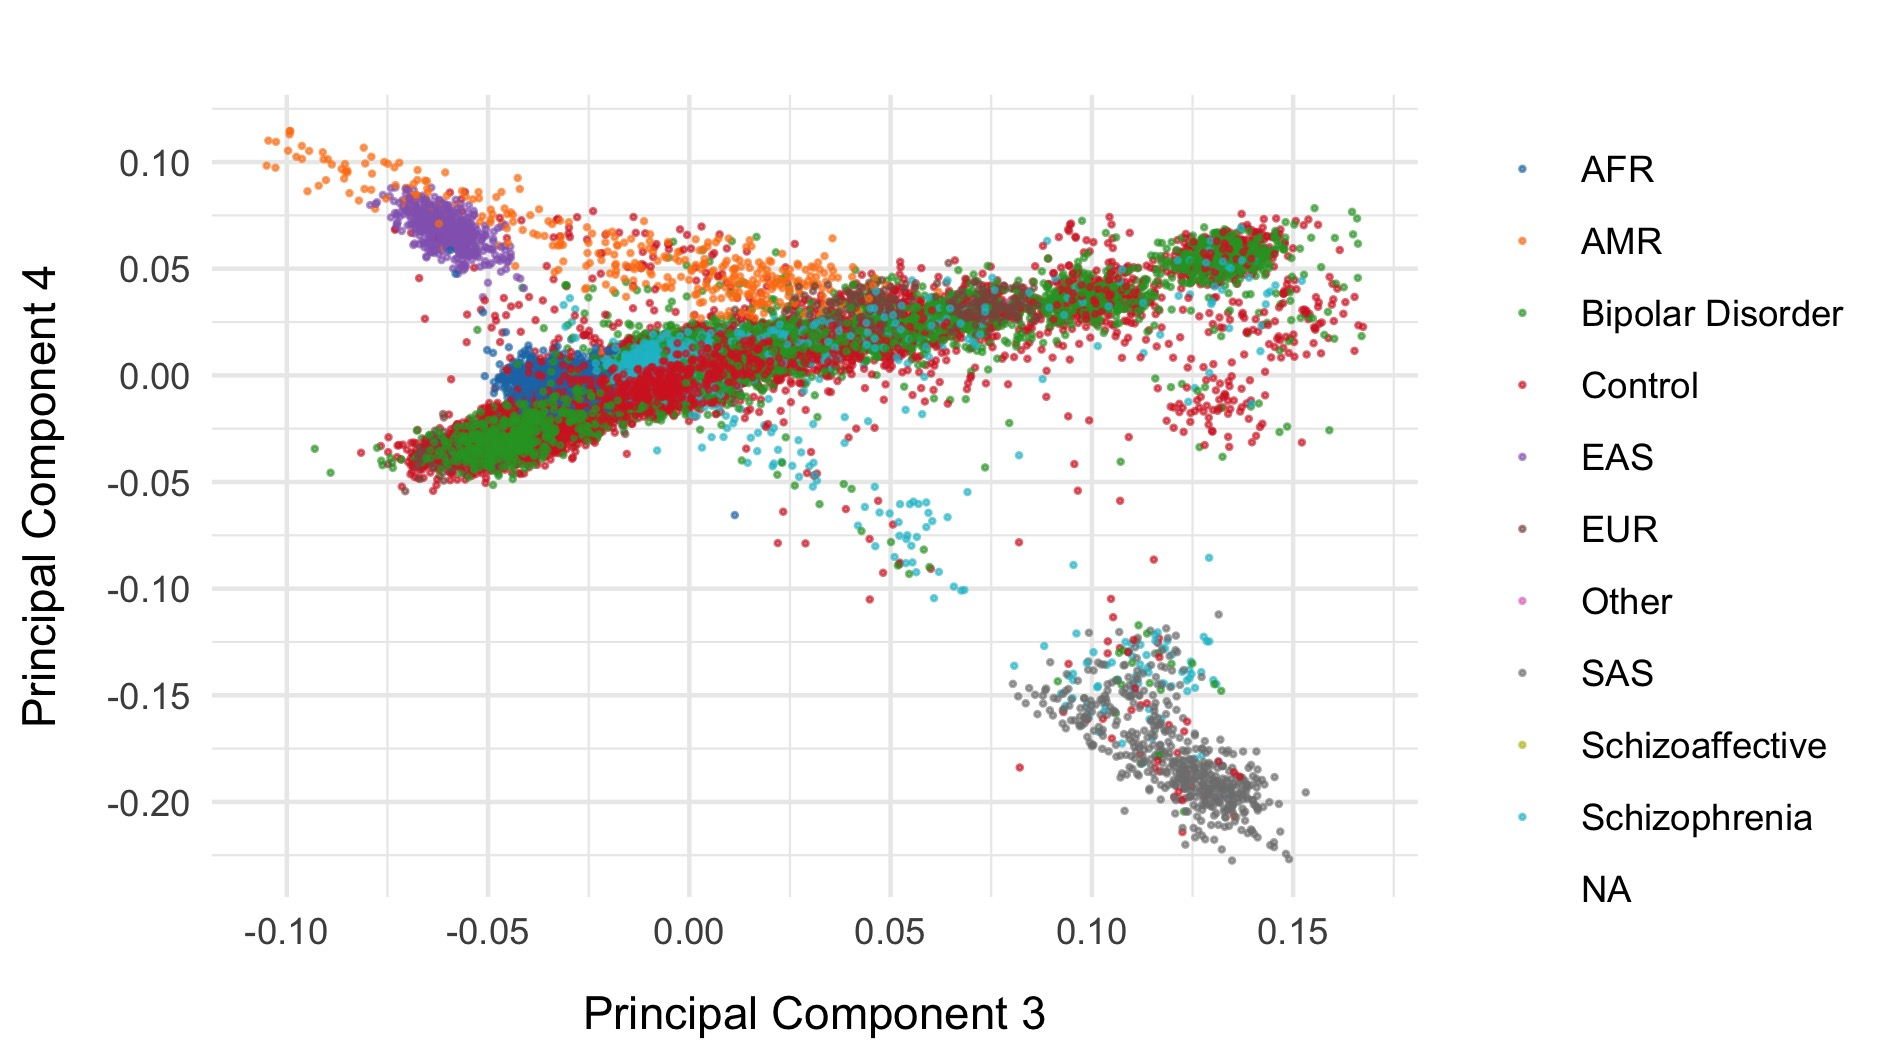
\includegraphics[width=0.5\textwidth]{10_PC3_PC4_1kg.jpg}}
\subfloat{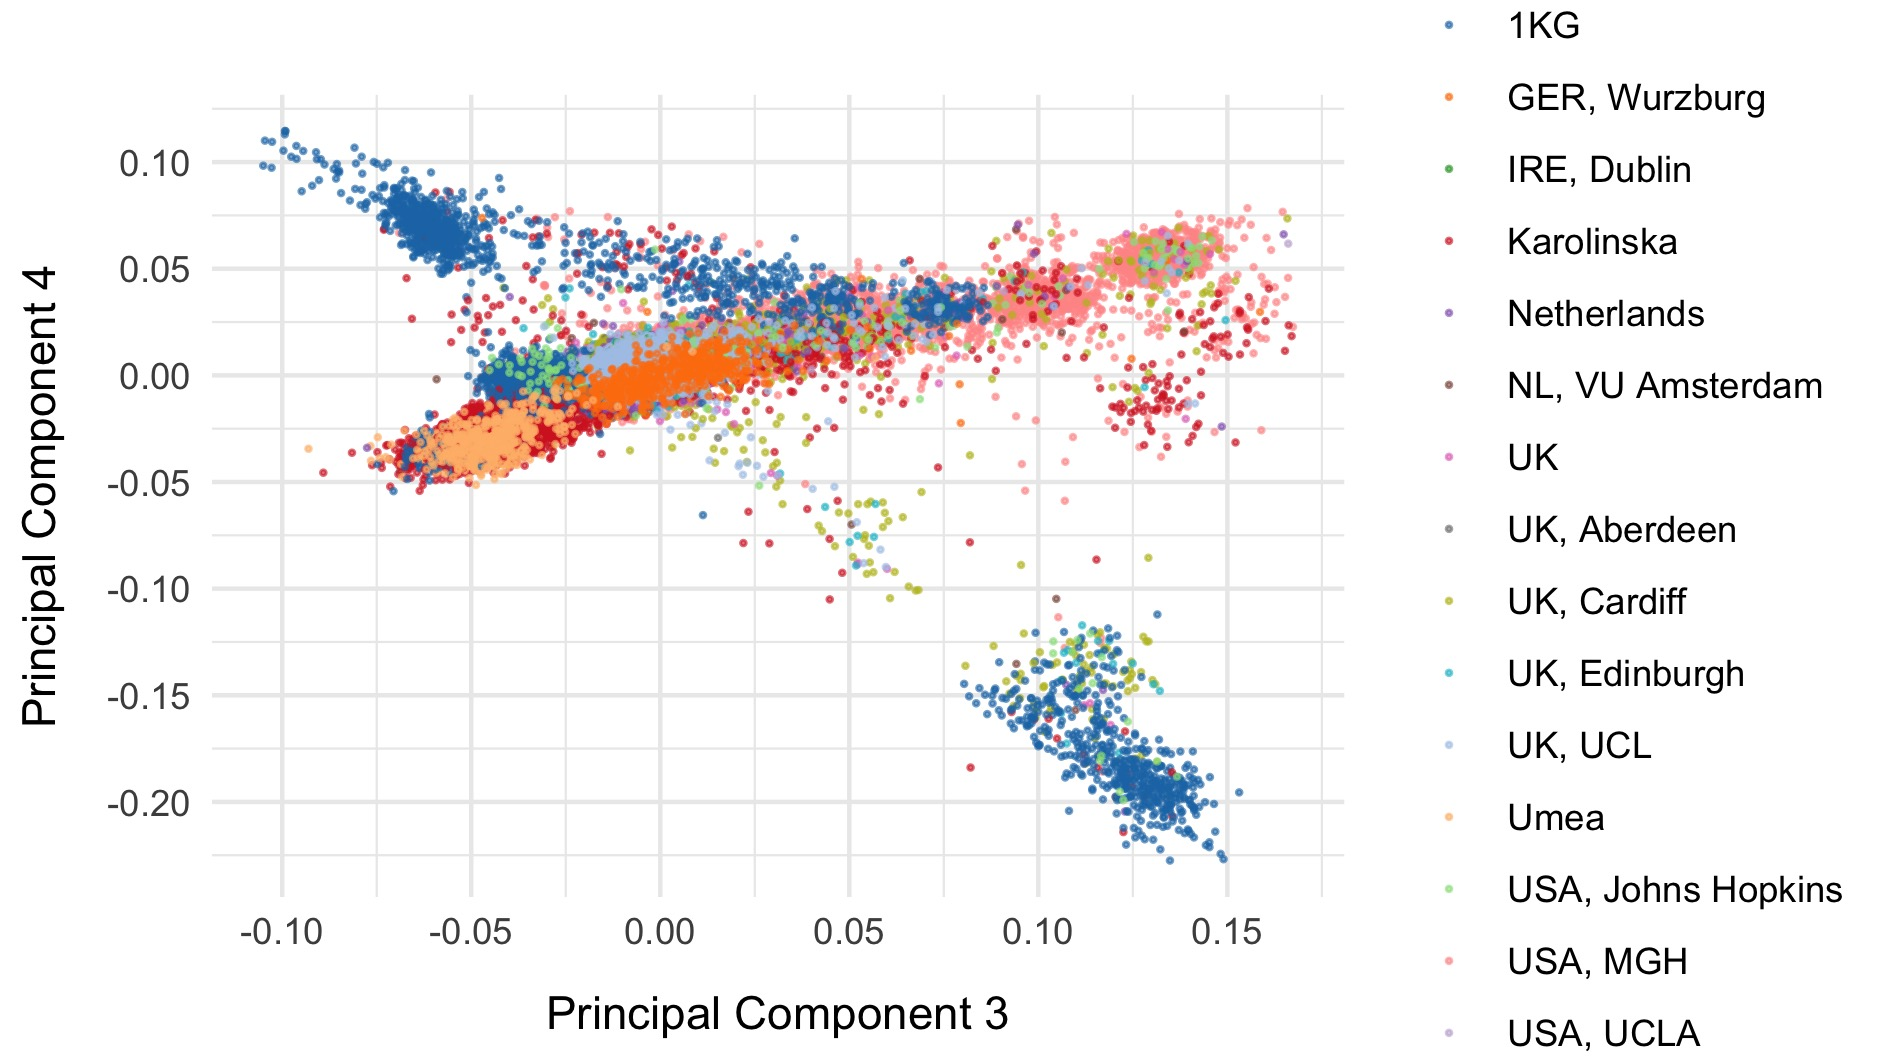
\includegraphics[width=0.5\textwidth]{10_PC3_PC4_1kg_collection.jpg}}\\
\subfloat{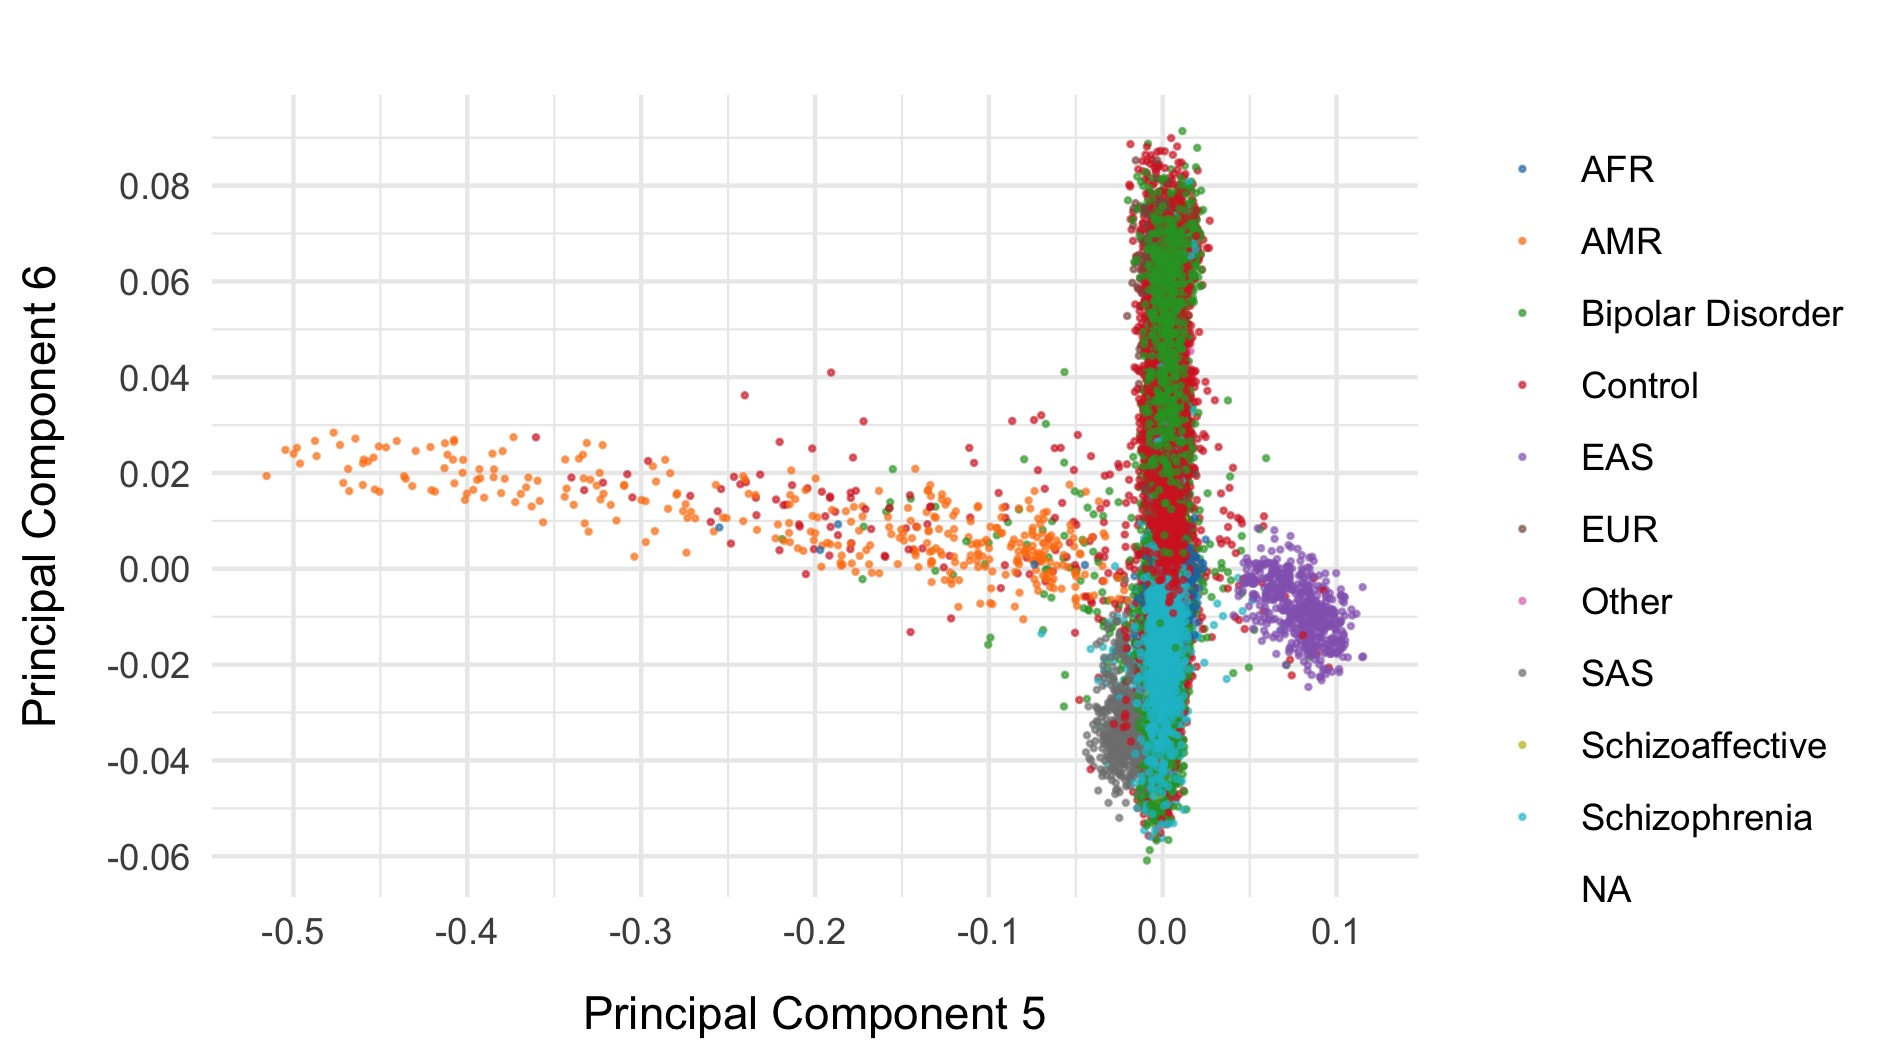
\includegraphics[width=0.5\textwidth]{10_PC5_PC6_1kg.jpg}}
\subfloat{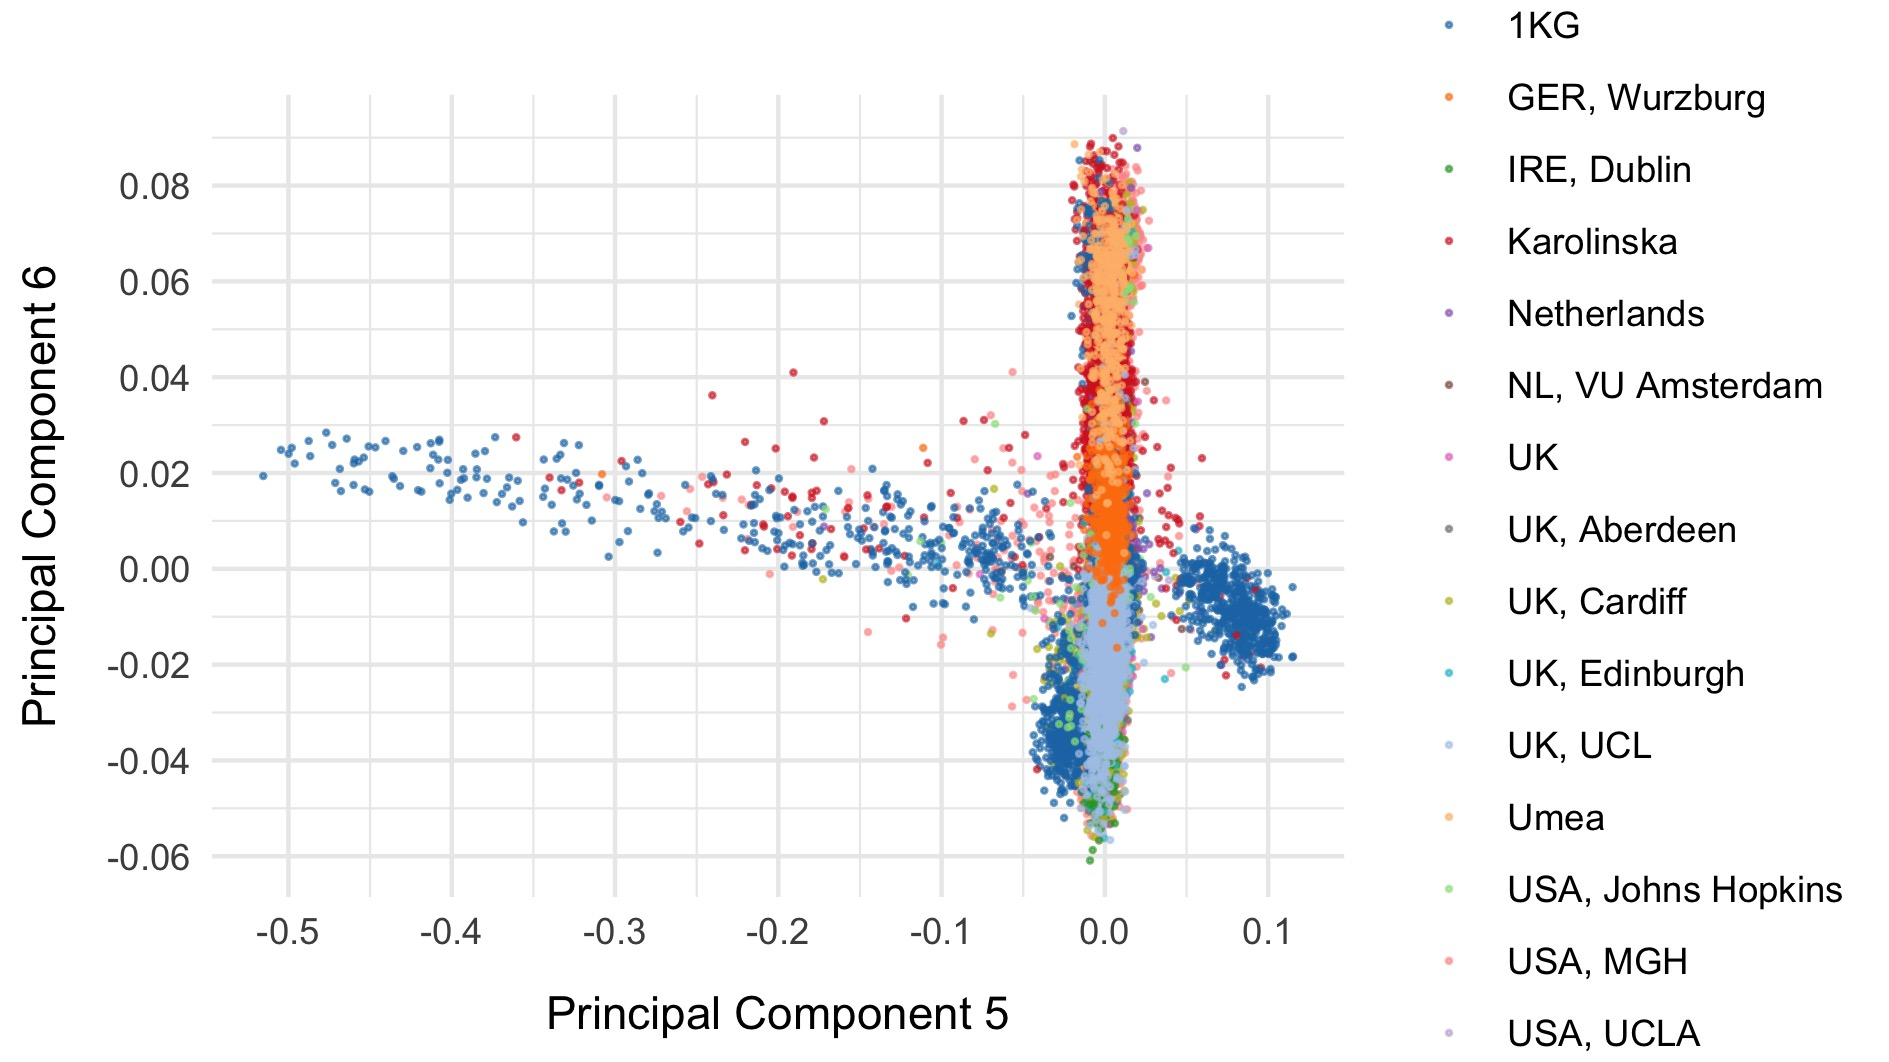
\includegraphics[width=0.5\textwidth]{10_PC5_PC6_1kg_collection.jpg}}
\caption{Initial PCA of all samples with 1000 Genomes}
\label{fig:PCA_1kg}
\end{figure}

\begin{figure}
\centering
\subfloat{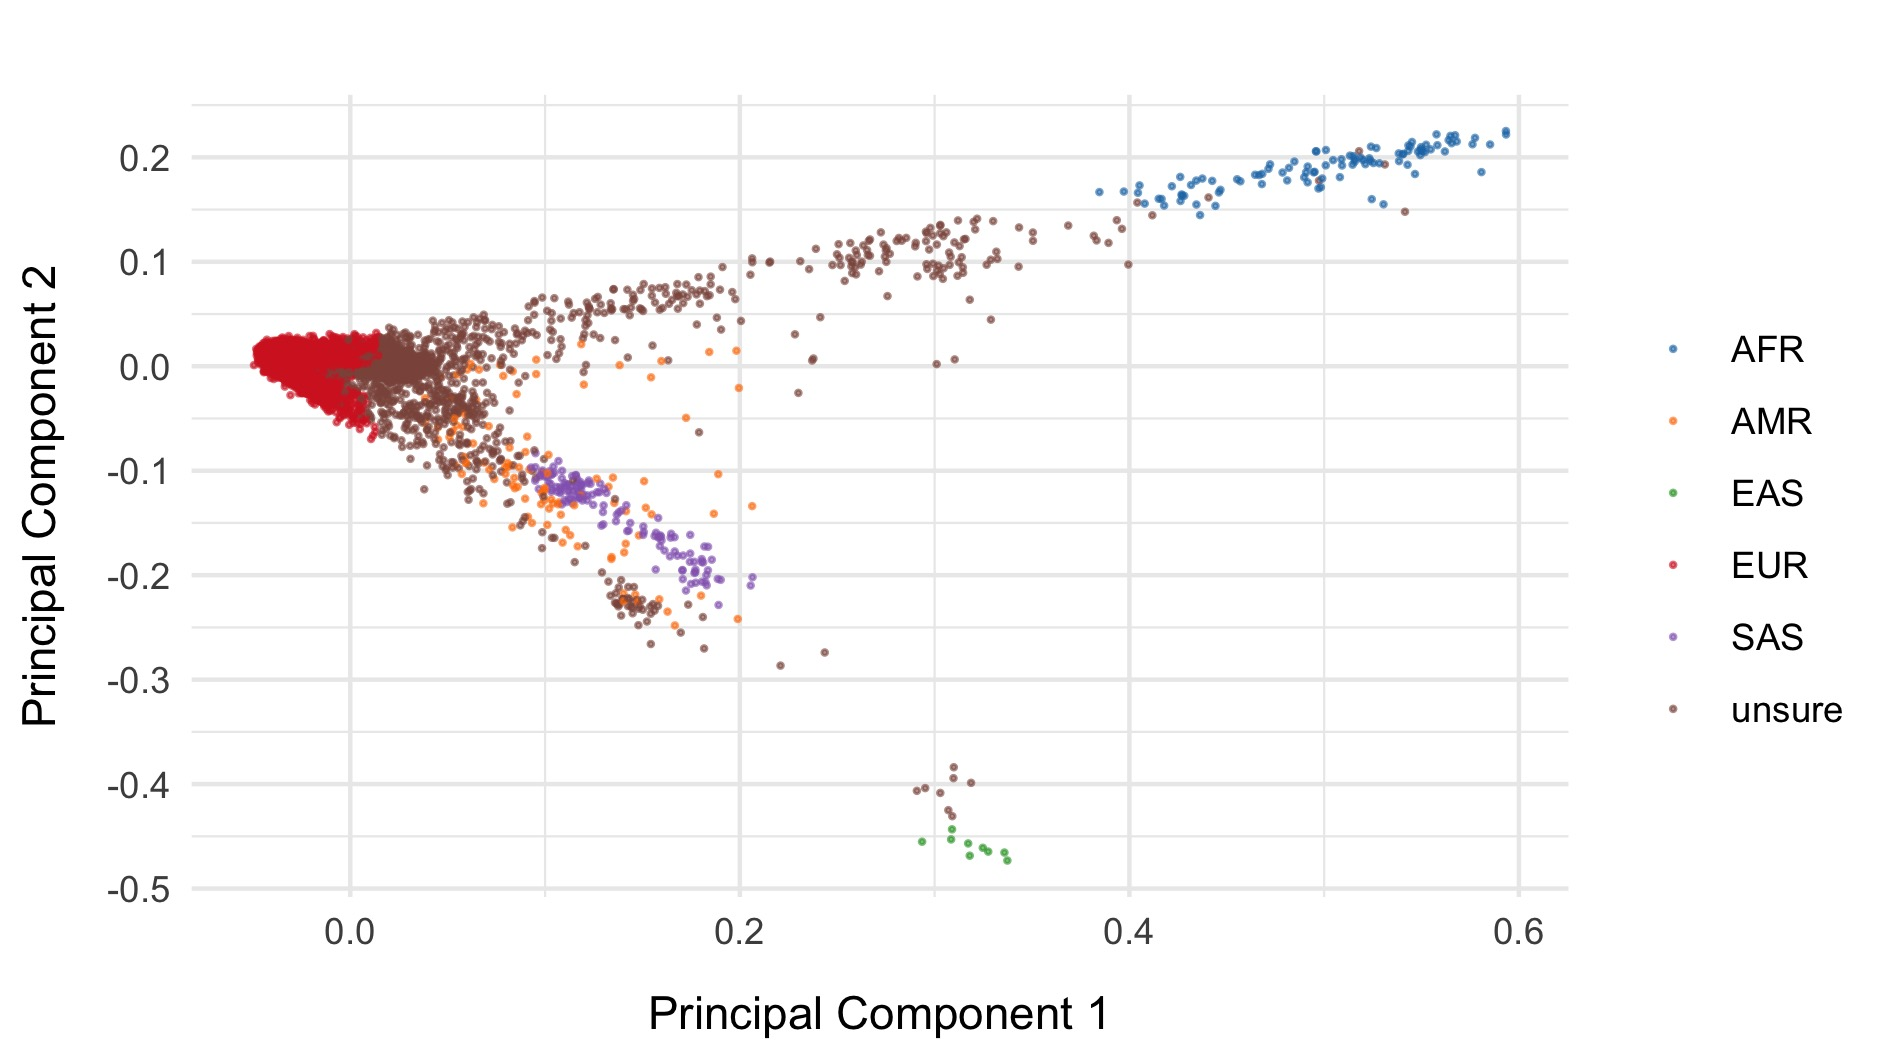
\includegraphics[width=0.5\textwidth]{10_PC1_PC2_classify_EUR_strict.jpg}}
\subfloat{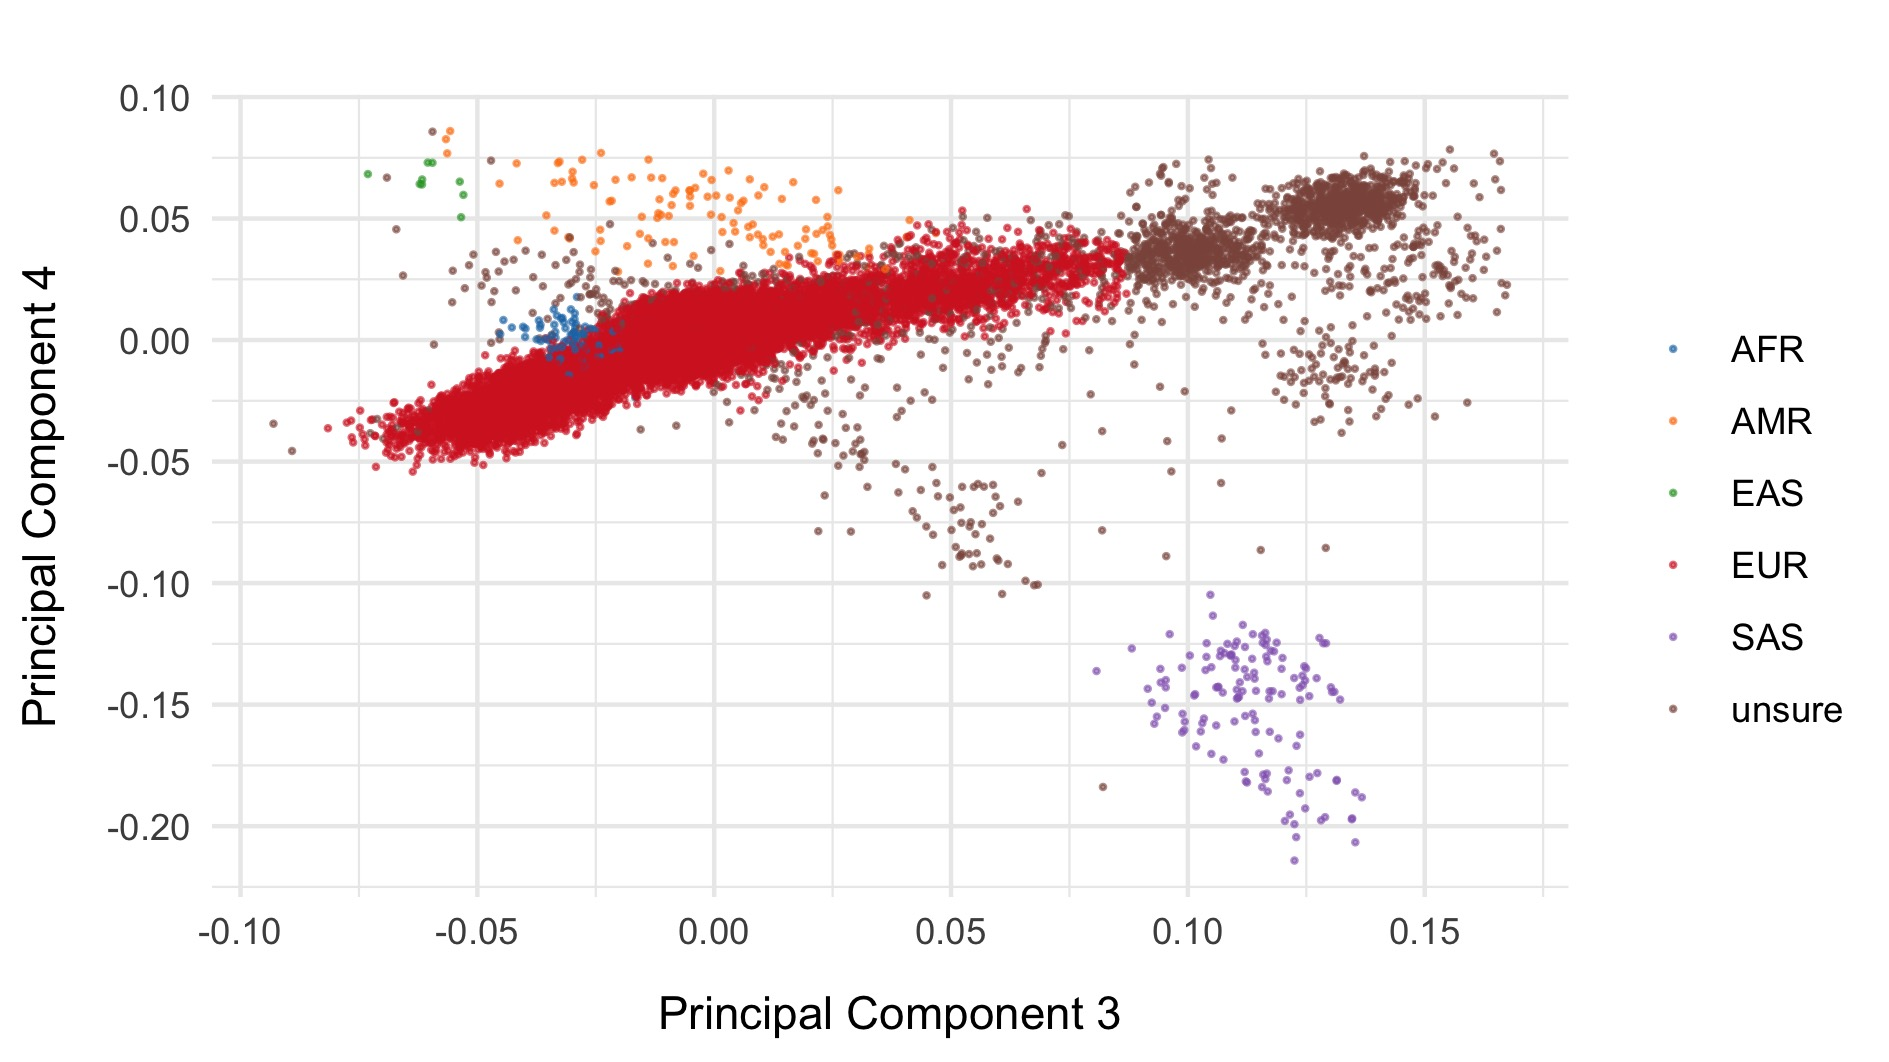
\includegraphics[width=0.5\textwidth]{10_PC3_PC4_classify_EUR_strict.jpg}}\\
\subfloat{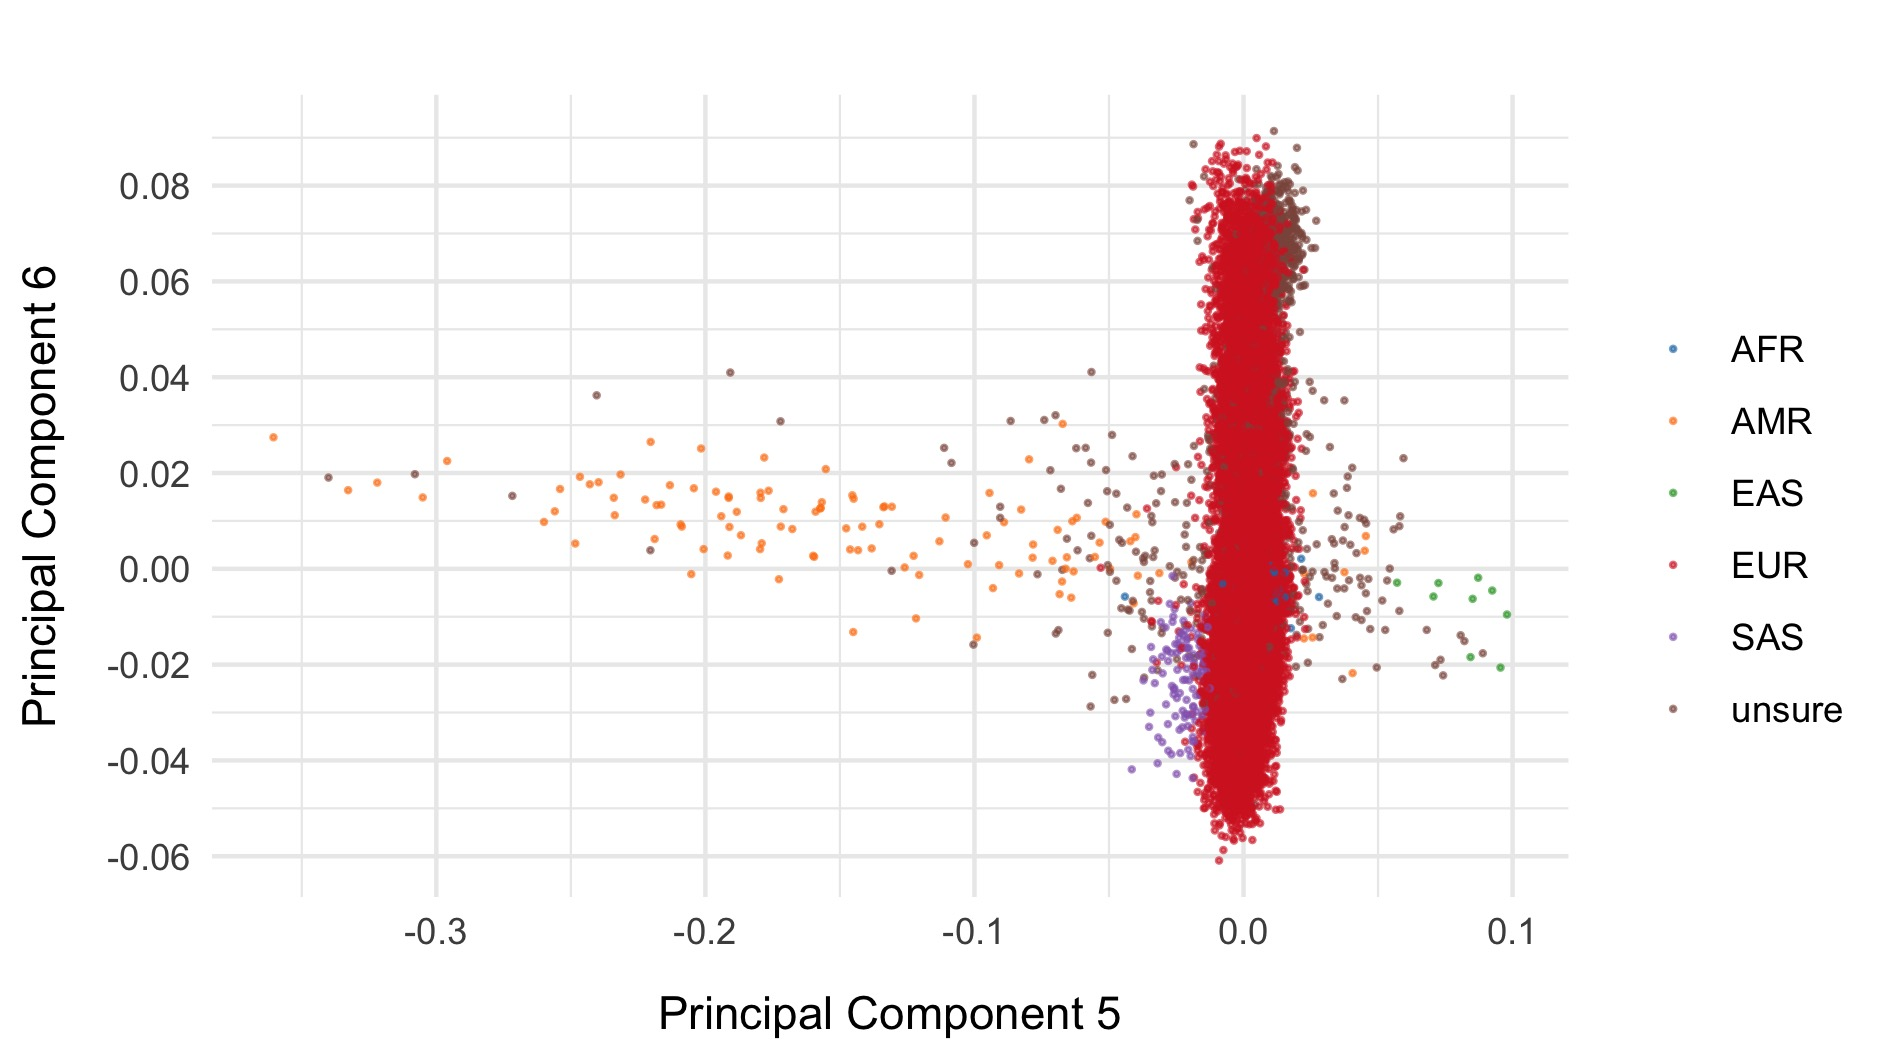
\includegraphics[width=0.5\textwidth]{10_PC5_PC6_classify_EUR_strict.jpg}}
\caption{Strict definition of European samples using random forest classifier, 500 trees. $P(European)>0.9$.}
\label{fig:PCA_1kg}
\end{figure}

% PCA europe.
\begin{figure}
\centering
\subfloat{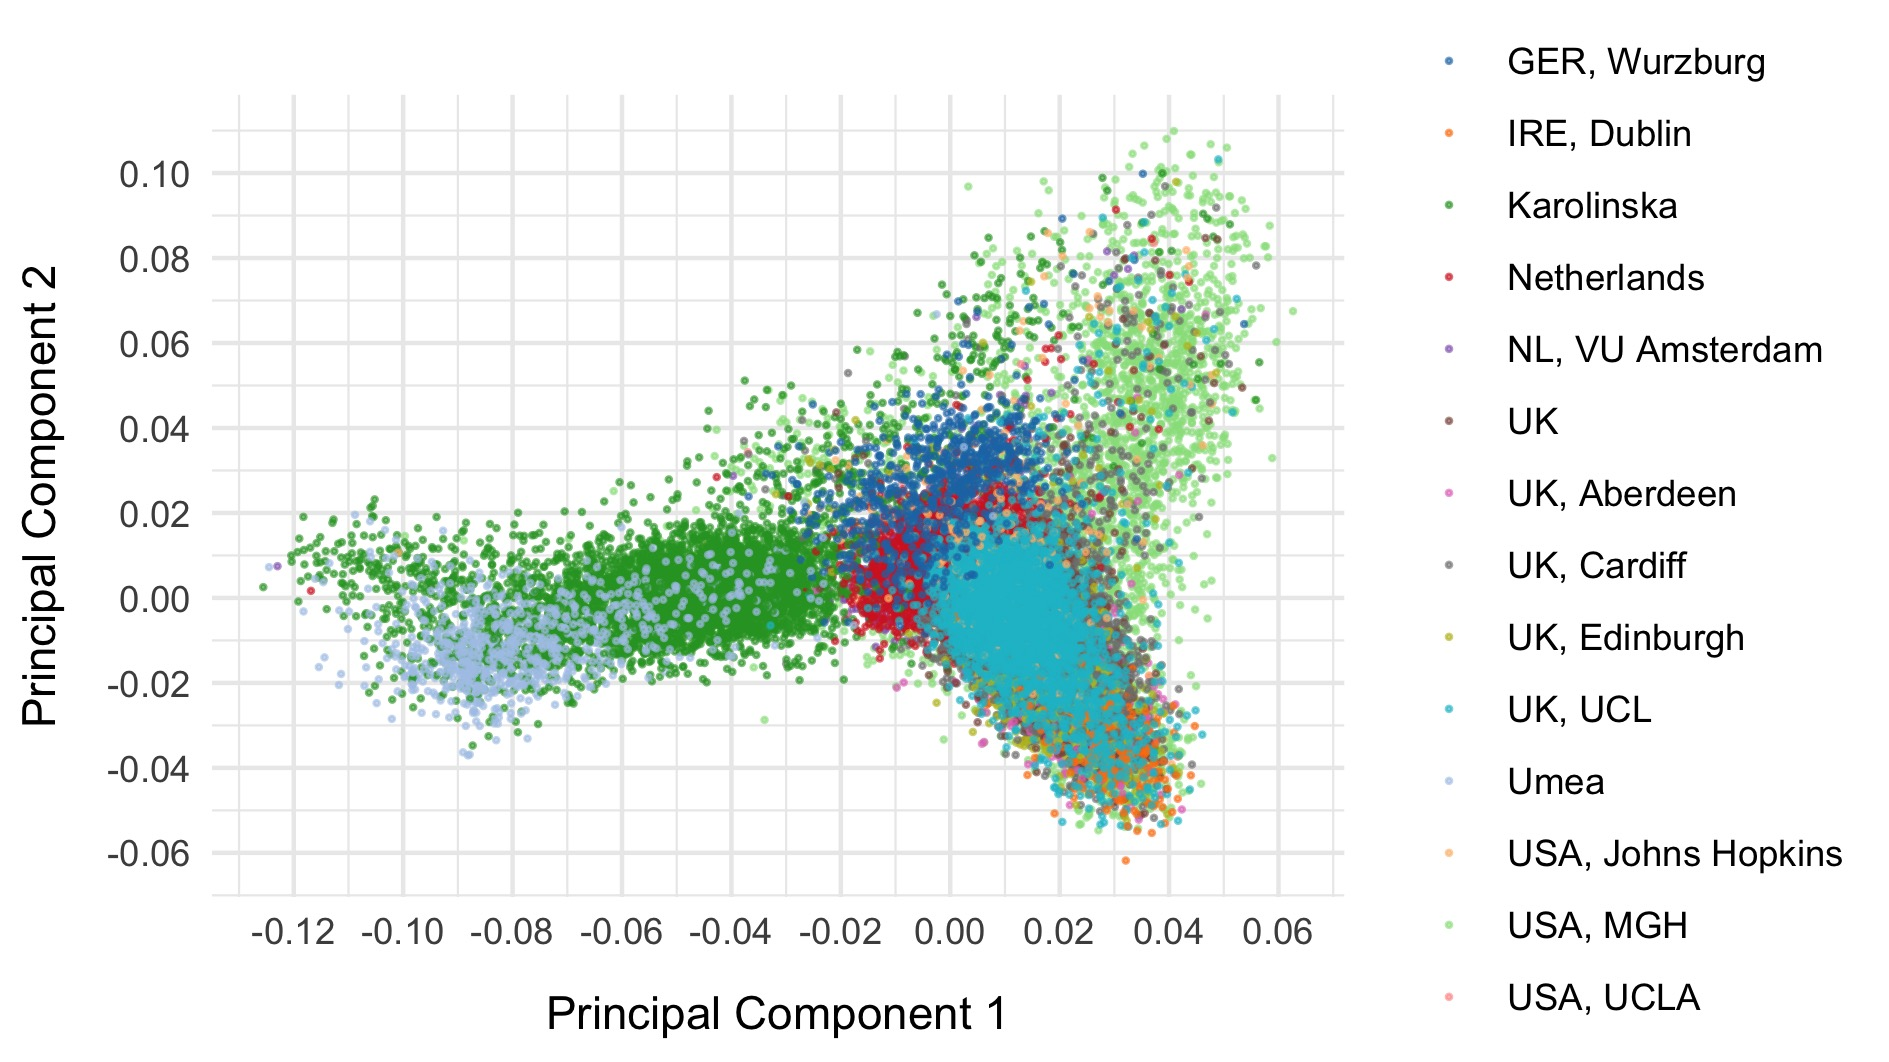
\includegraphics[width=0.5\textwidth]{11_PC1_PC2_EUR.jpg}}
\subfloat{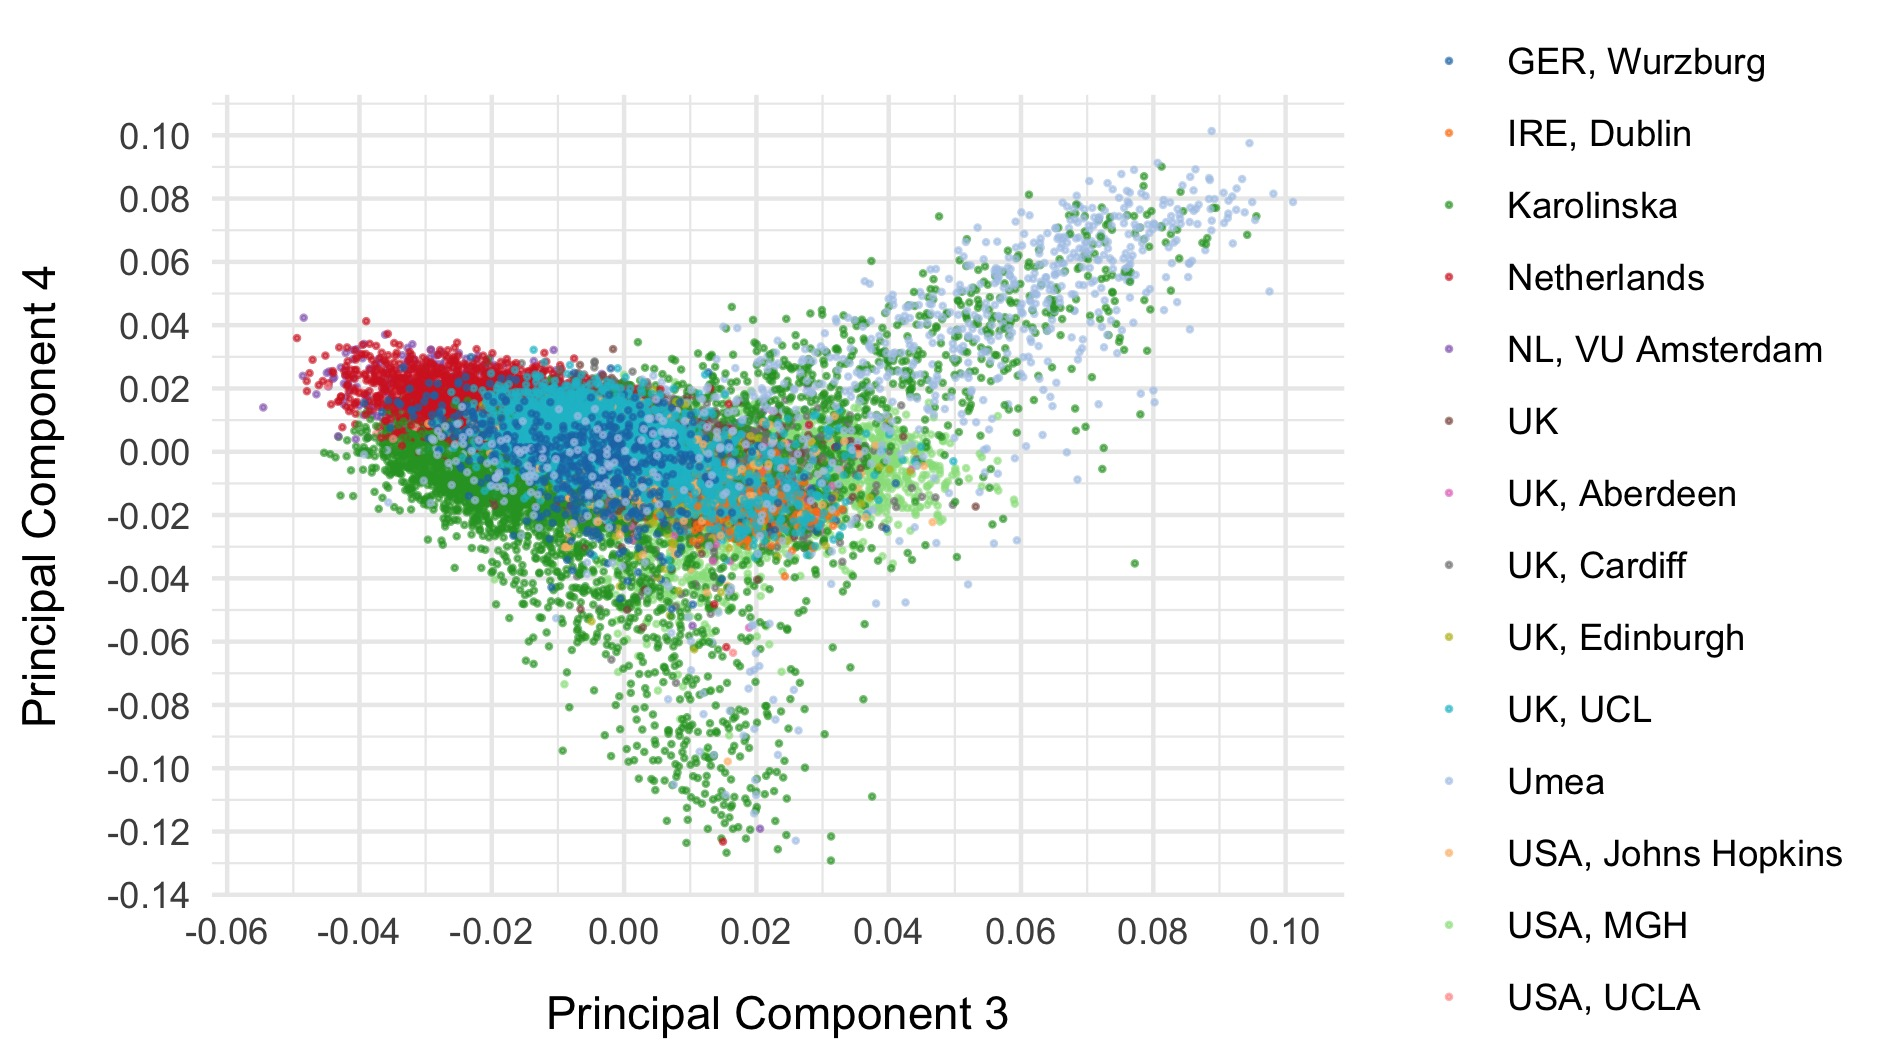
\includegraphics[width=0.5\textwidth]{11_PC3_PC4_EUR.jpg}}\\
\subfloat{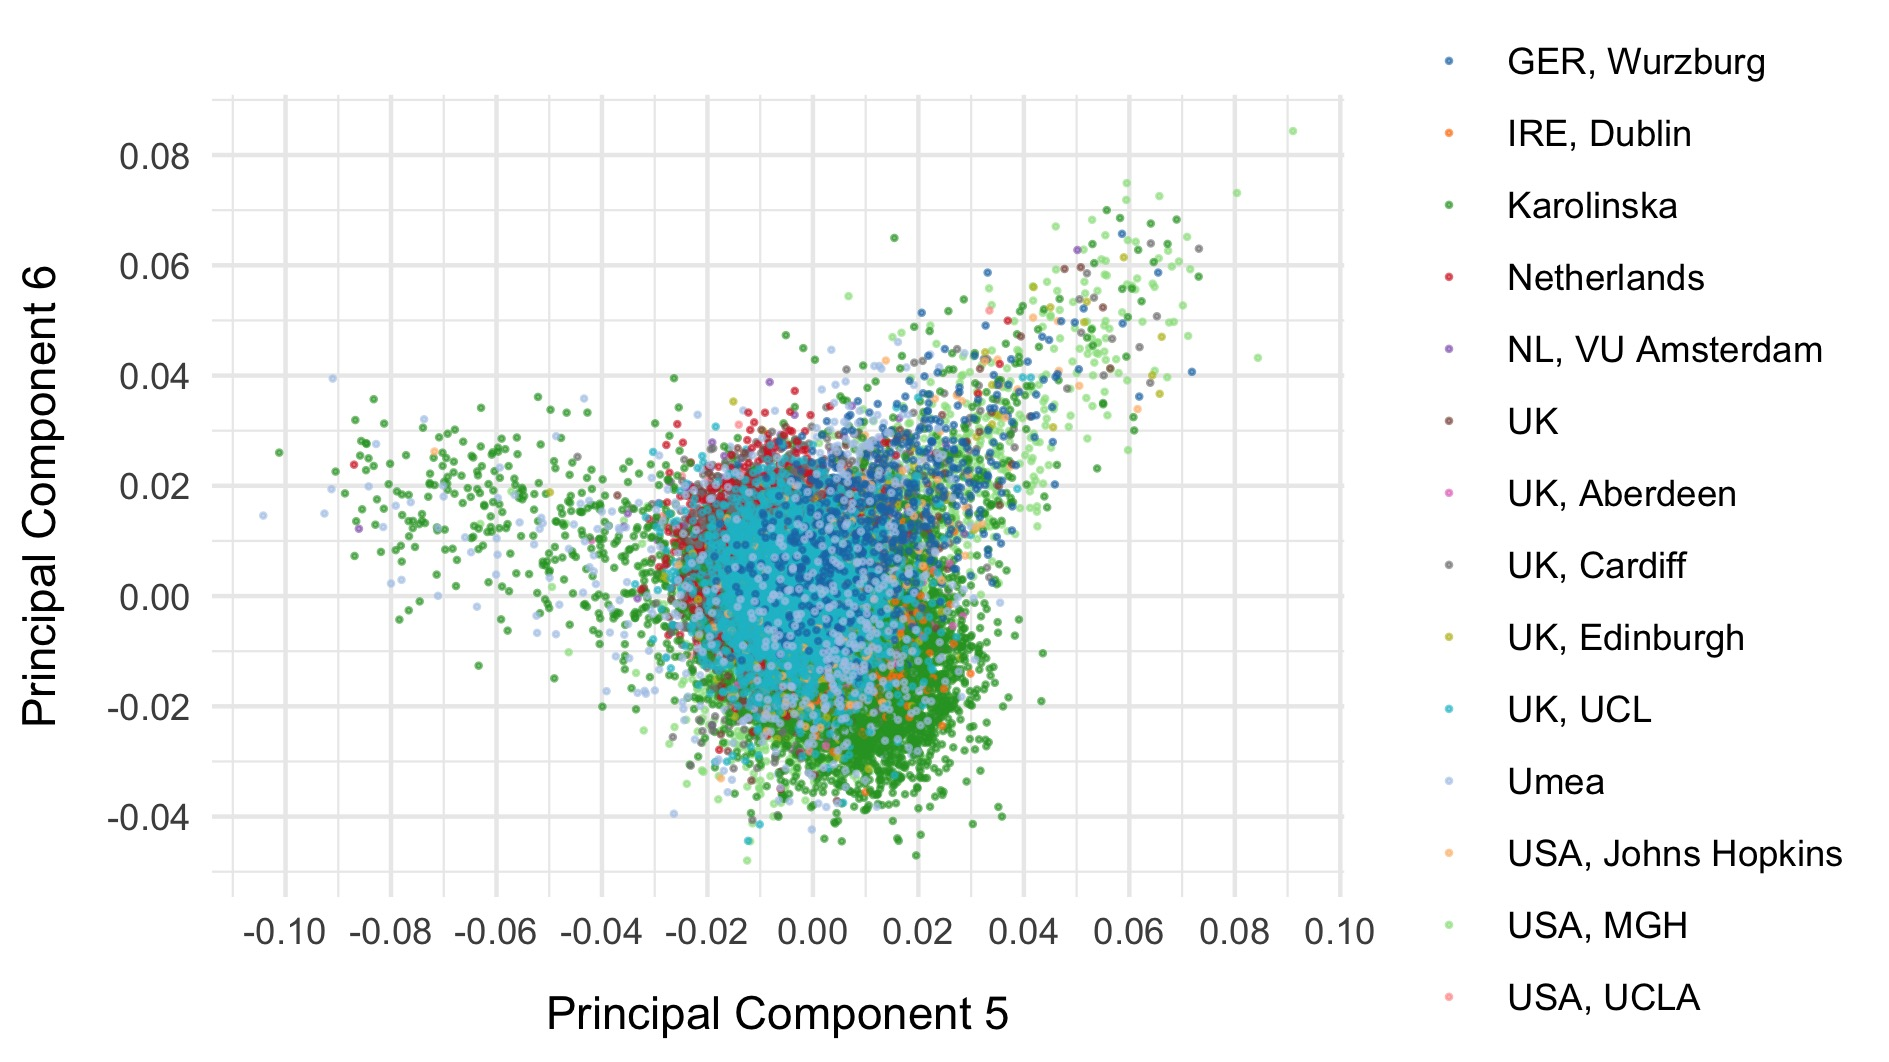
\includegraphics[width=0.5\textwidth]{11_PC5_PC6_EUR.jpg}}
\caption{PCA after restricting to strict European subset.}
\label{fig:PCA_EUR}
\end{figure}

% PCA AJ
\begin{figure}
\centering
\subfloat[AJ and half AJ cluster identified]{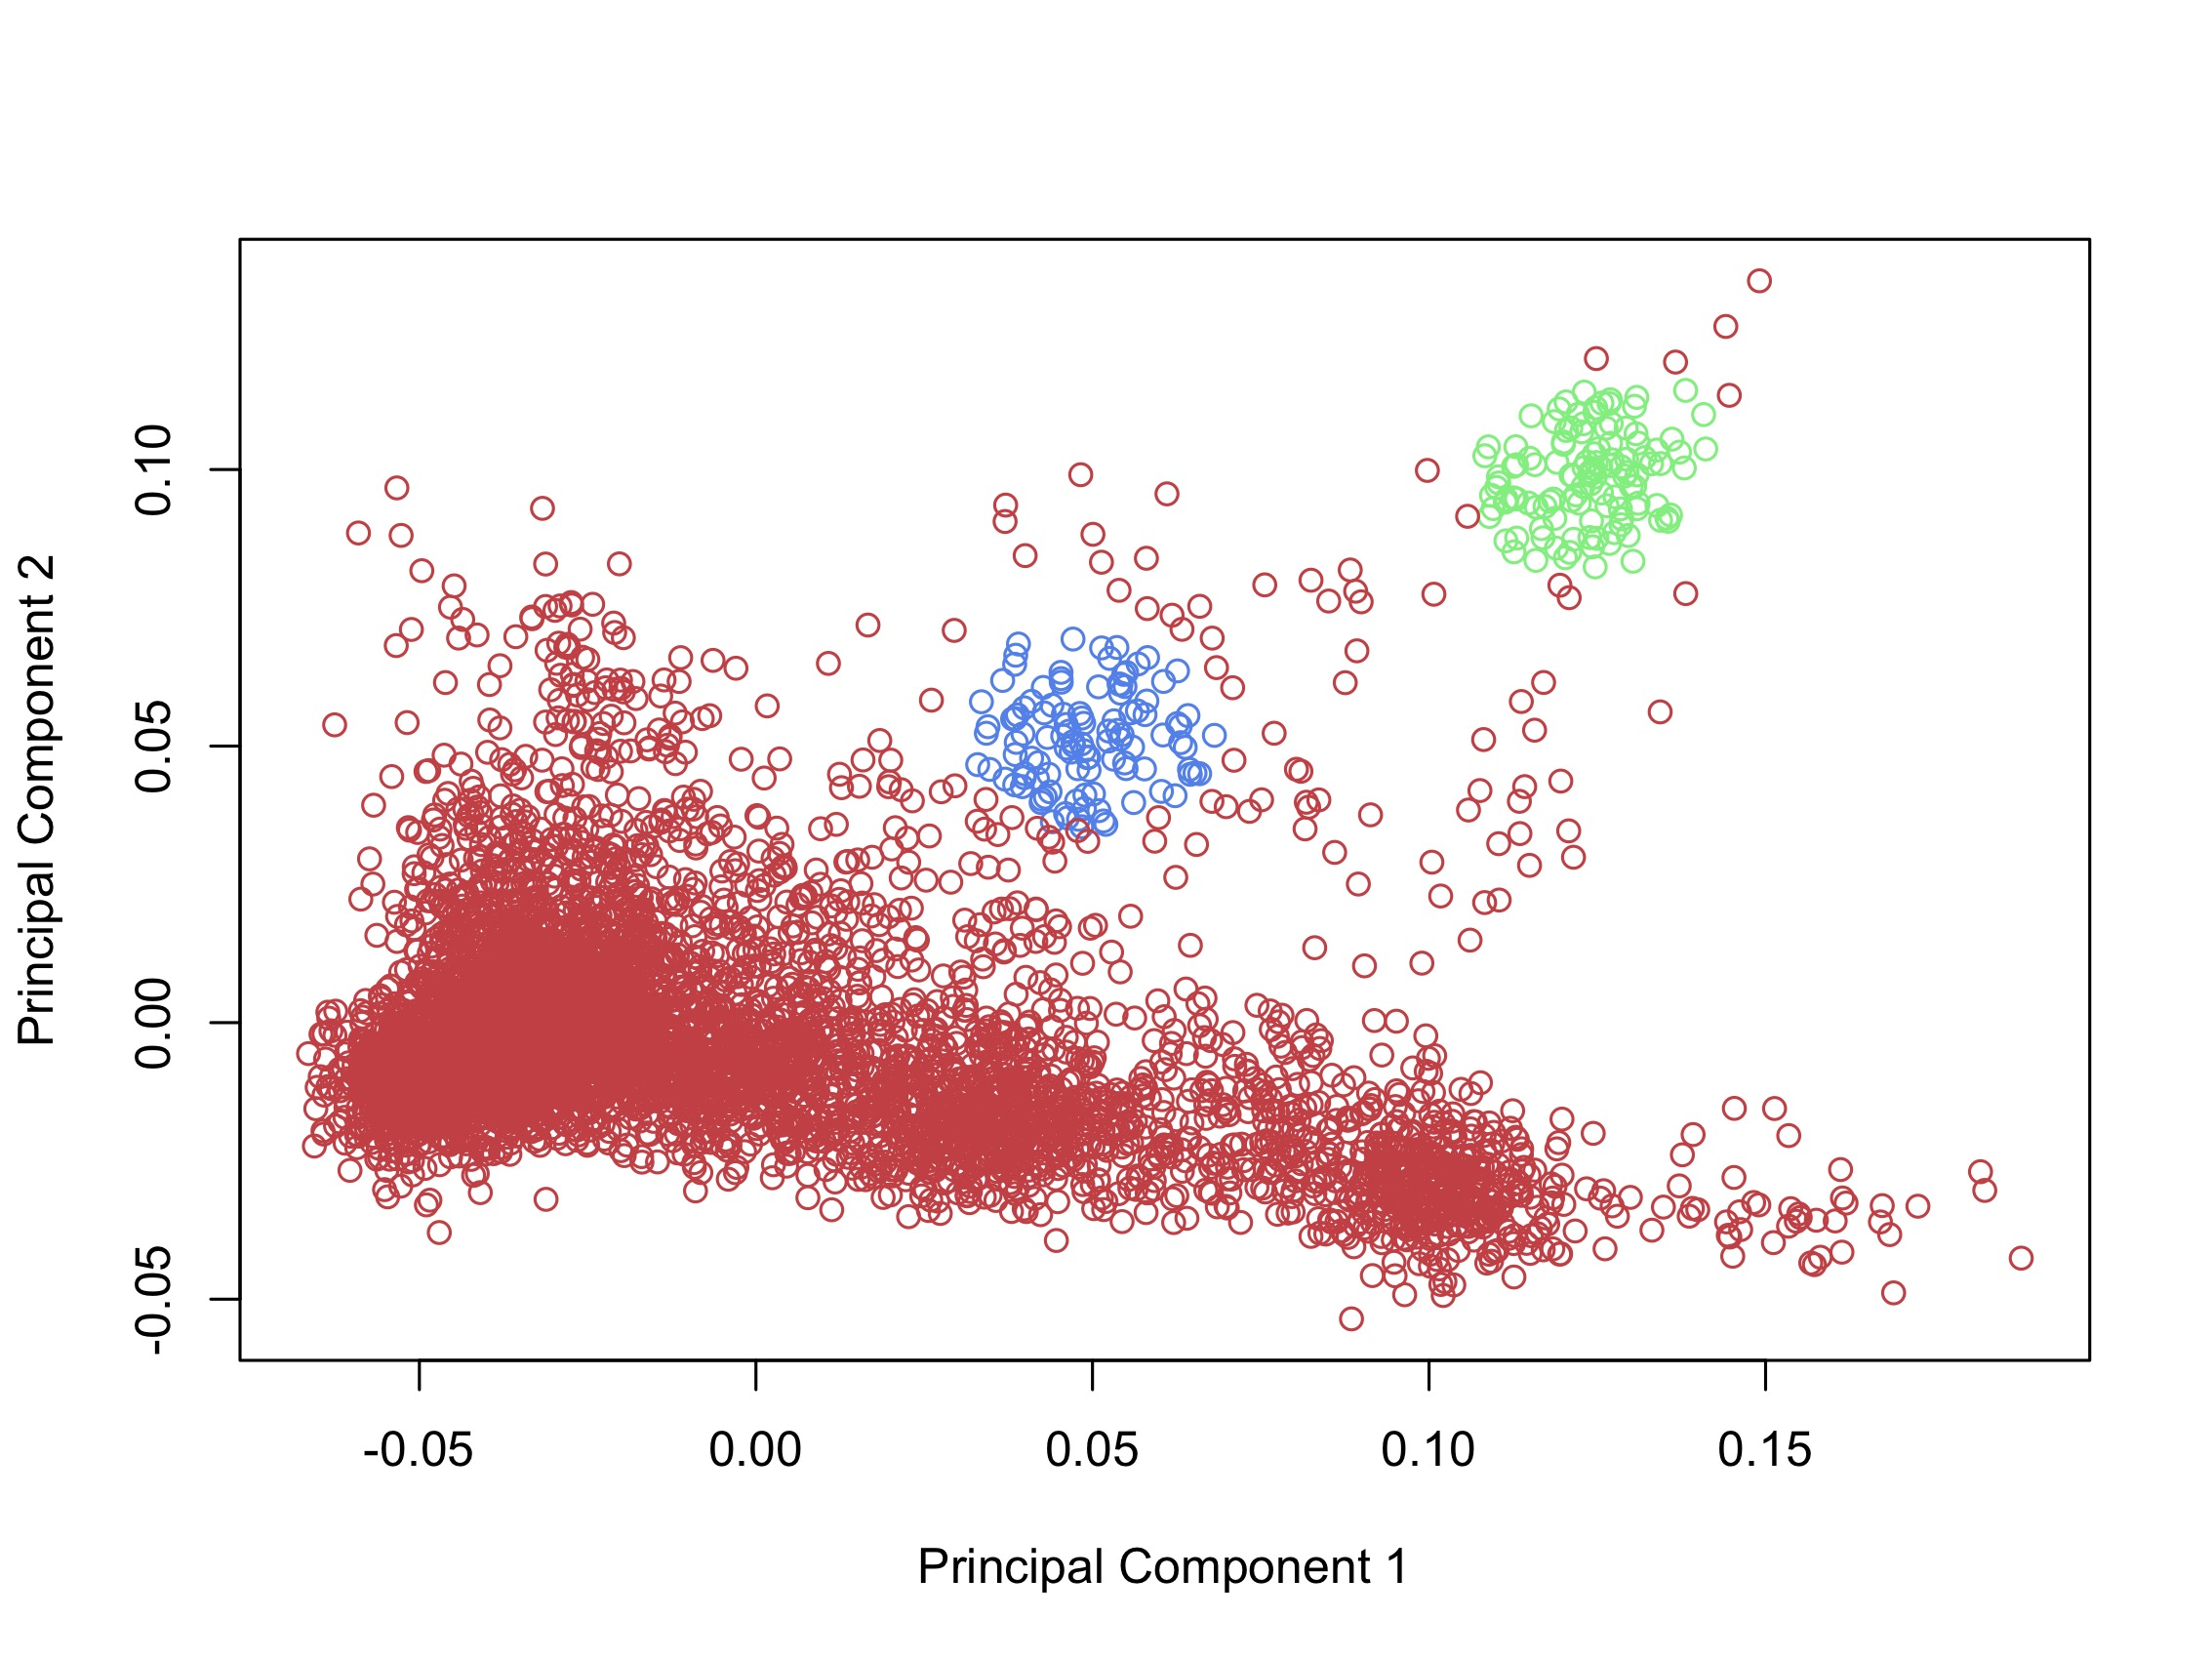
\includegraphics[width=0.5\textwidth]{12_AJ_in_US_PC1_PC2.jpg}}
\subfloat[Removal of outliers in US European samples]{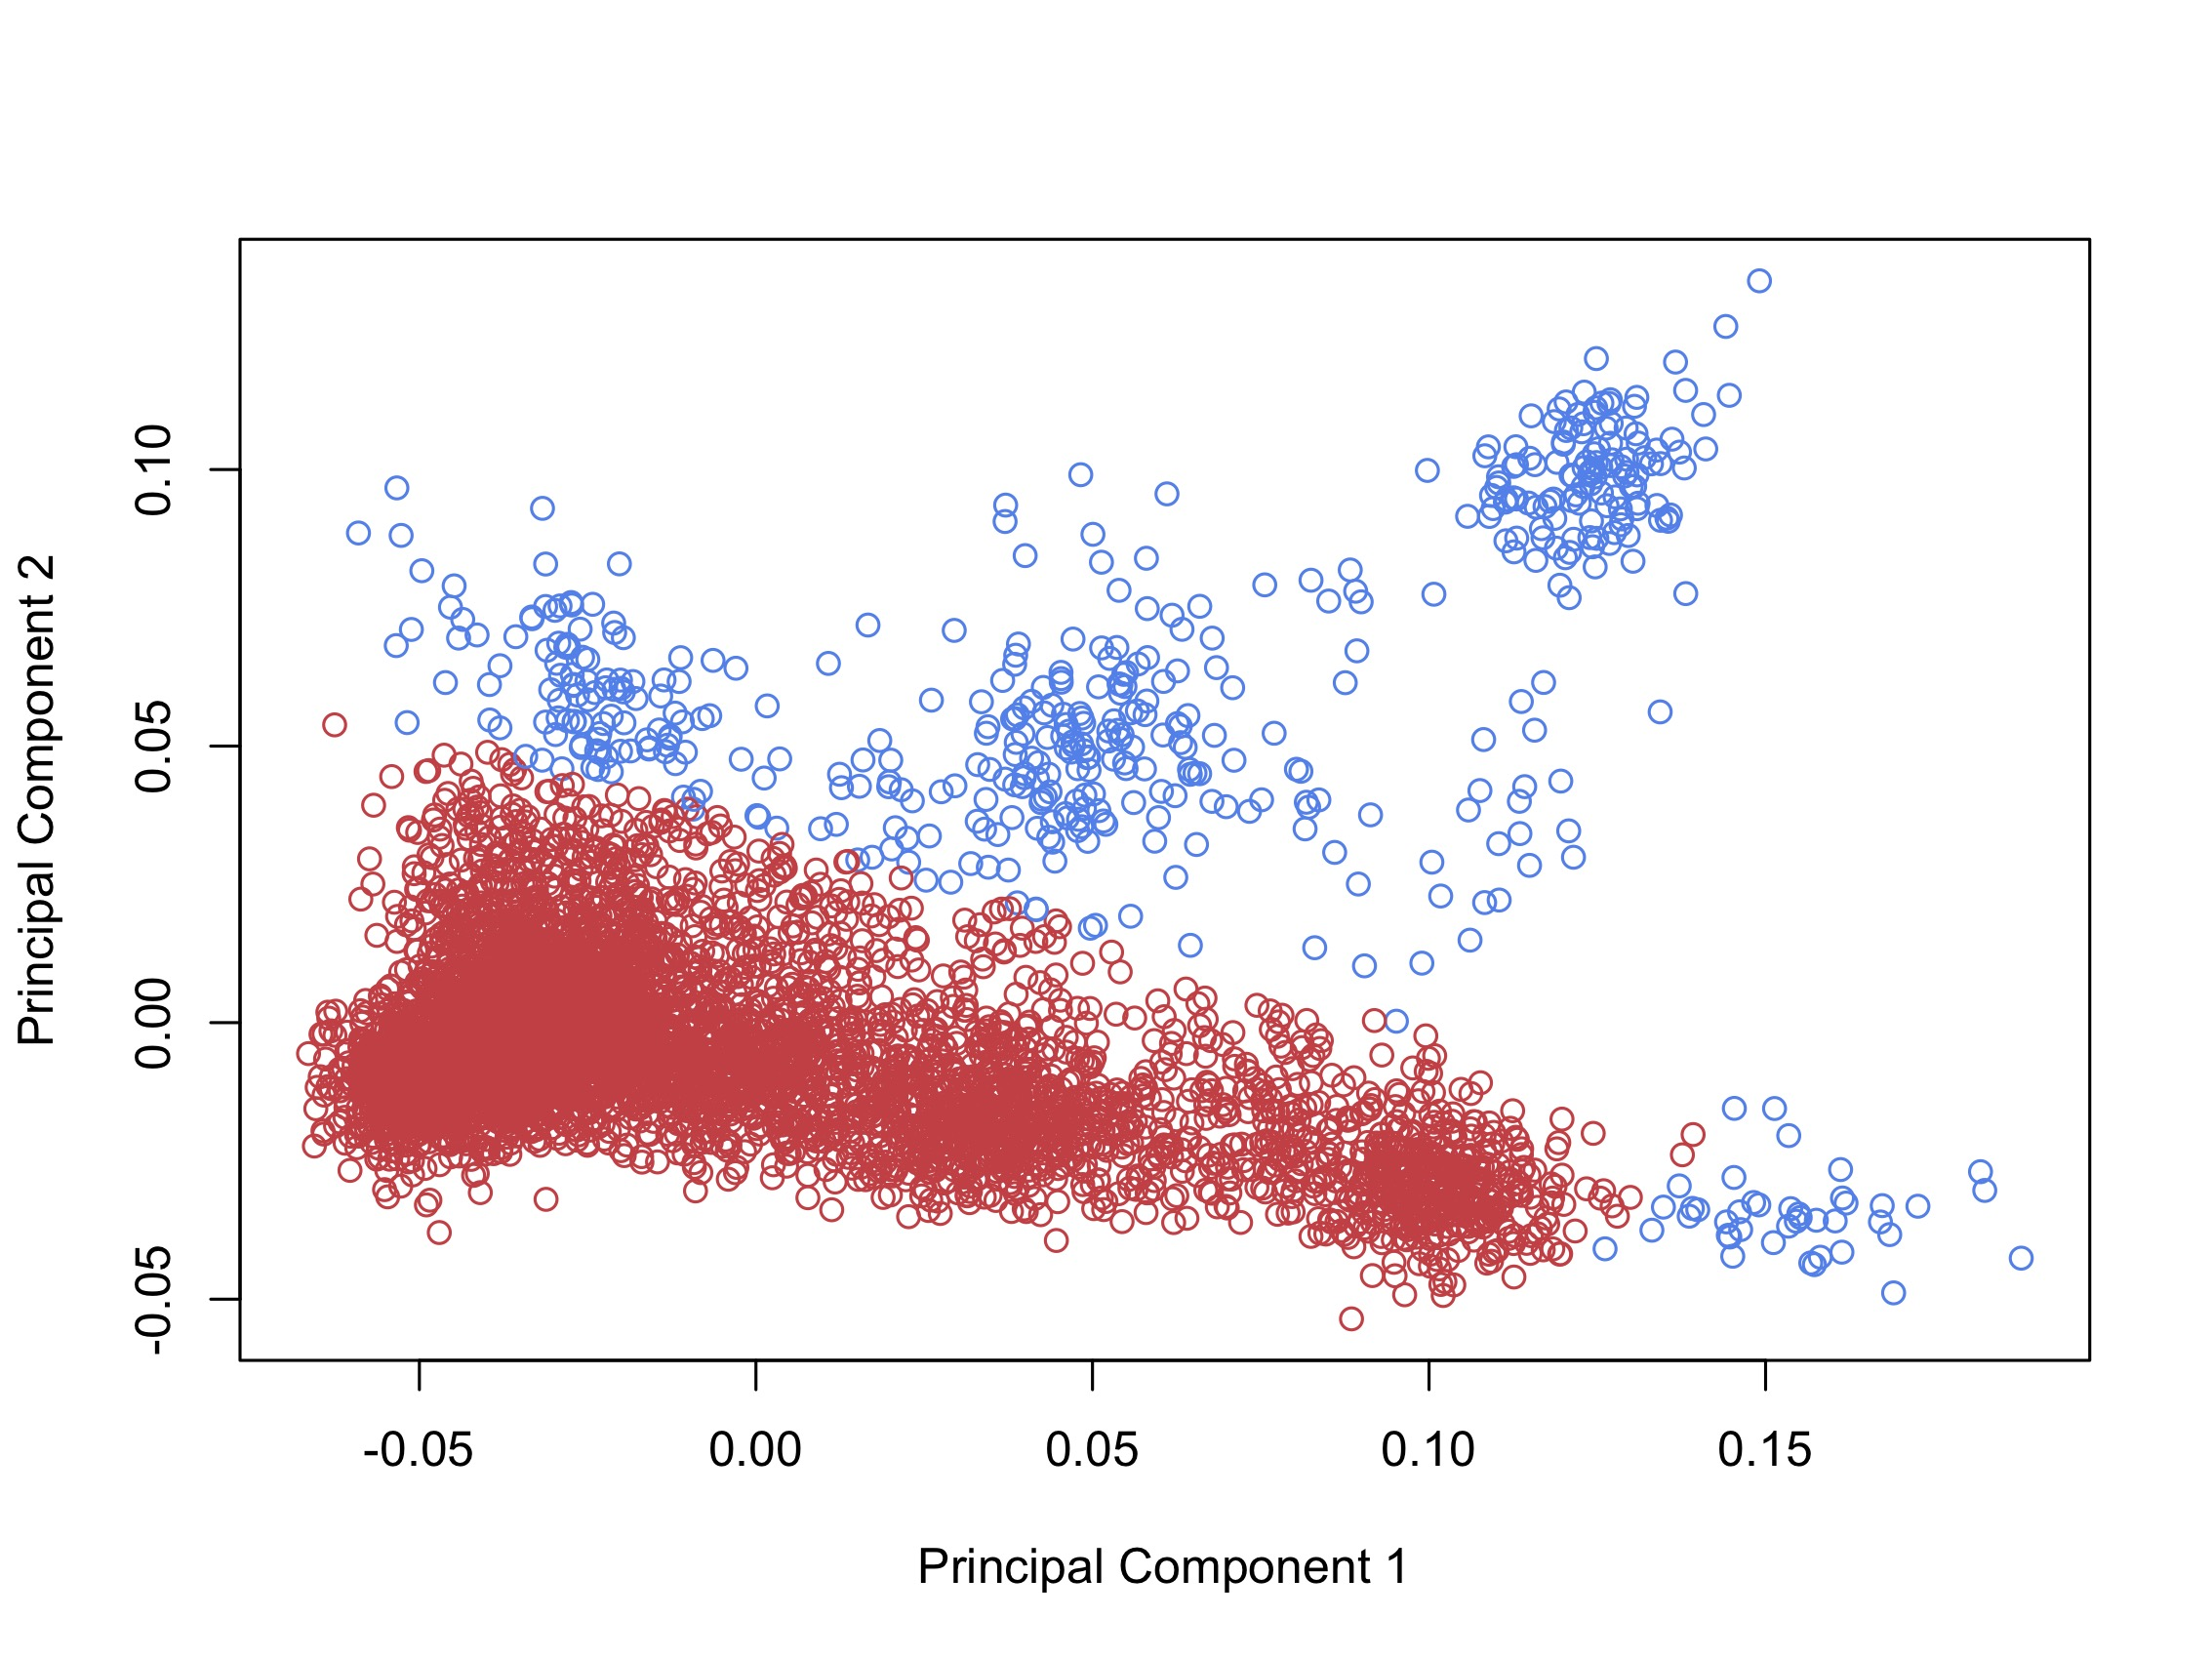
\includegraphics[width=0.5\textwidth]{12_AJ_remove_in_US_PC1_PC2.jpg}}
\caption{PCA of loosely defined `European' US samples to identify AJ cluster}
\label{fig:AJ_PCA}
\end{figure}

% PCA 1kg AJ
\begin{figure}
\centering
\subfloat{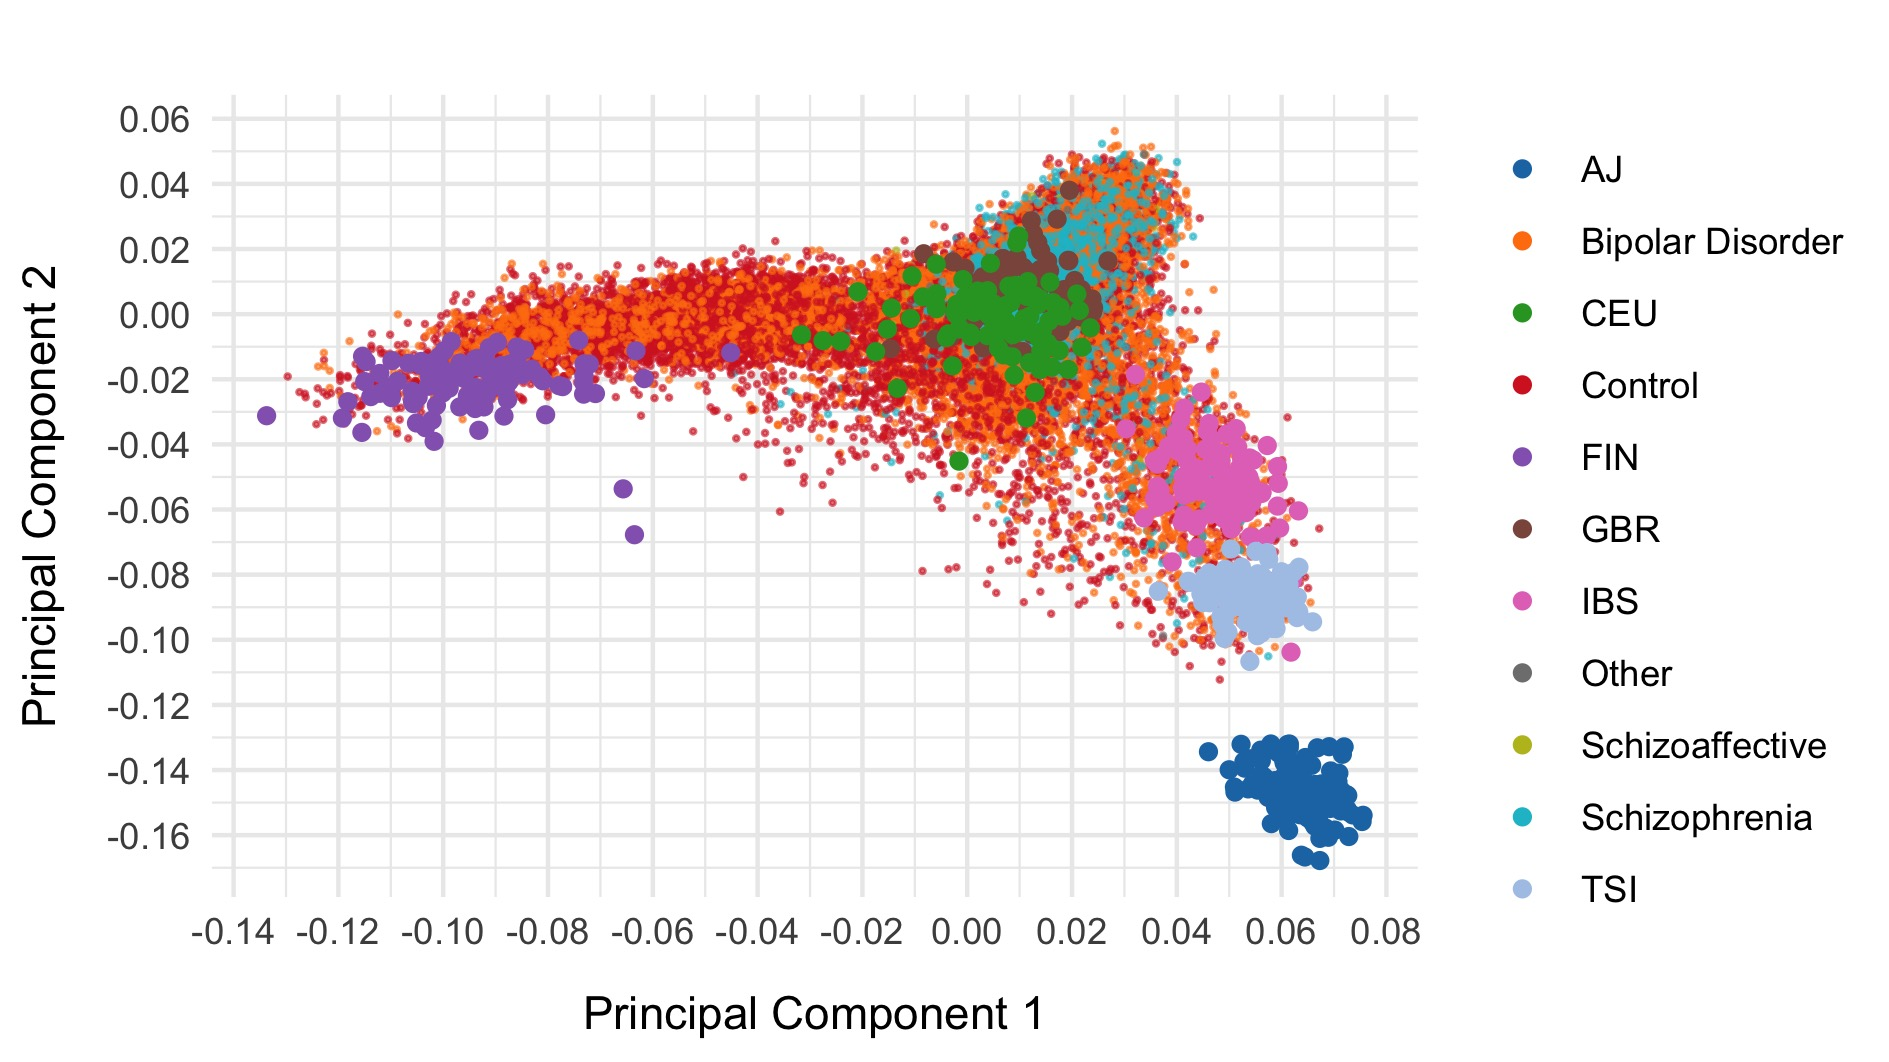
\includegraphics[width=0.5\textwidth]{13_PC1PC2_EUR_and_AJ_1kg.jpg}}
\subfloat{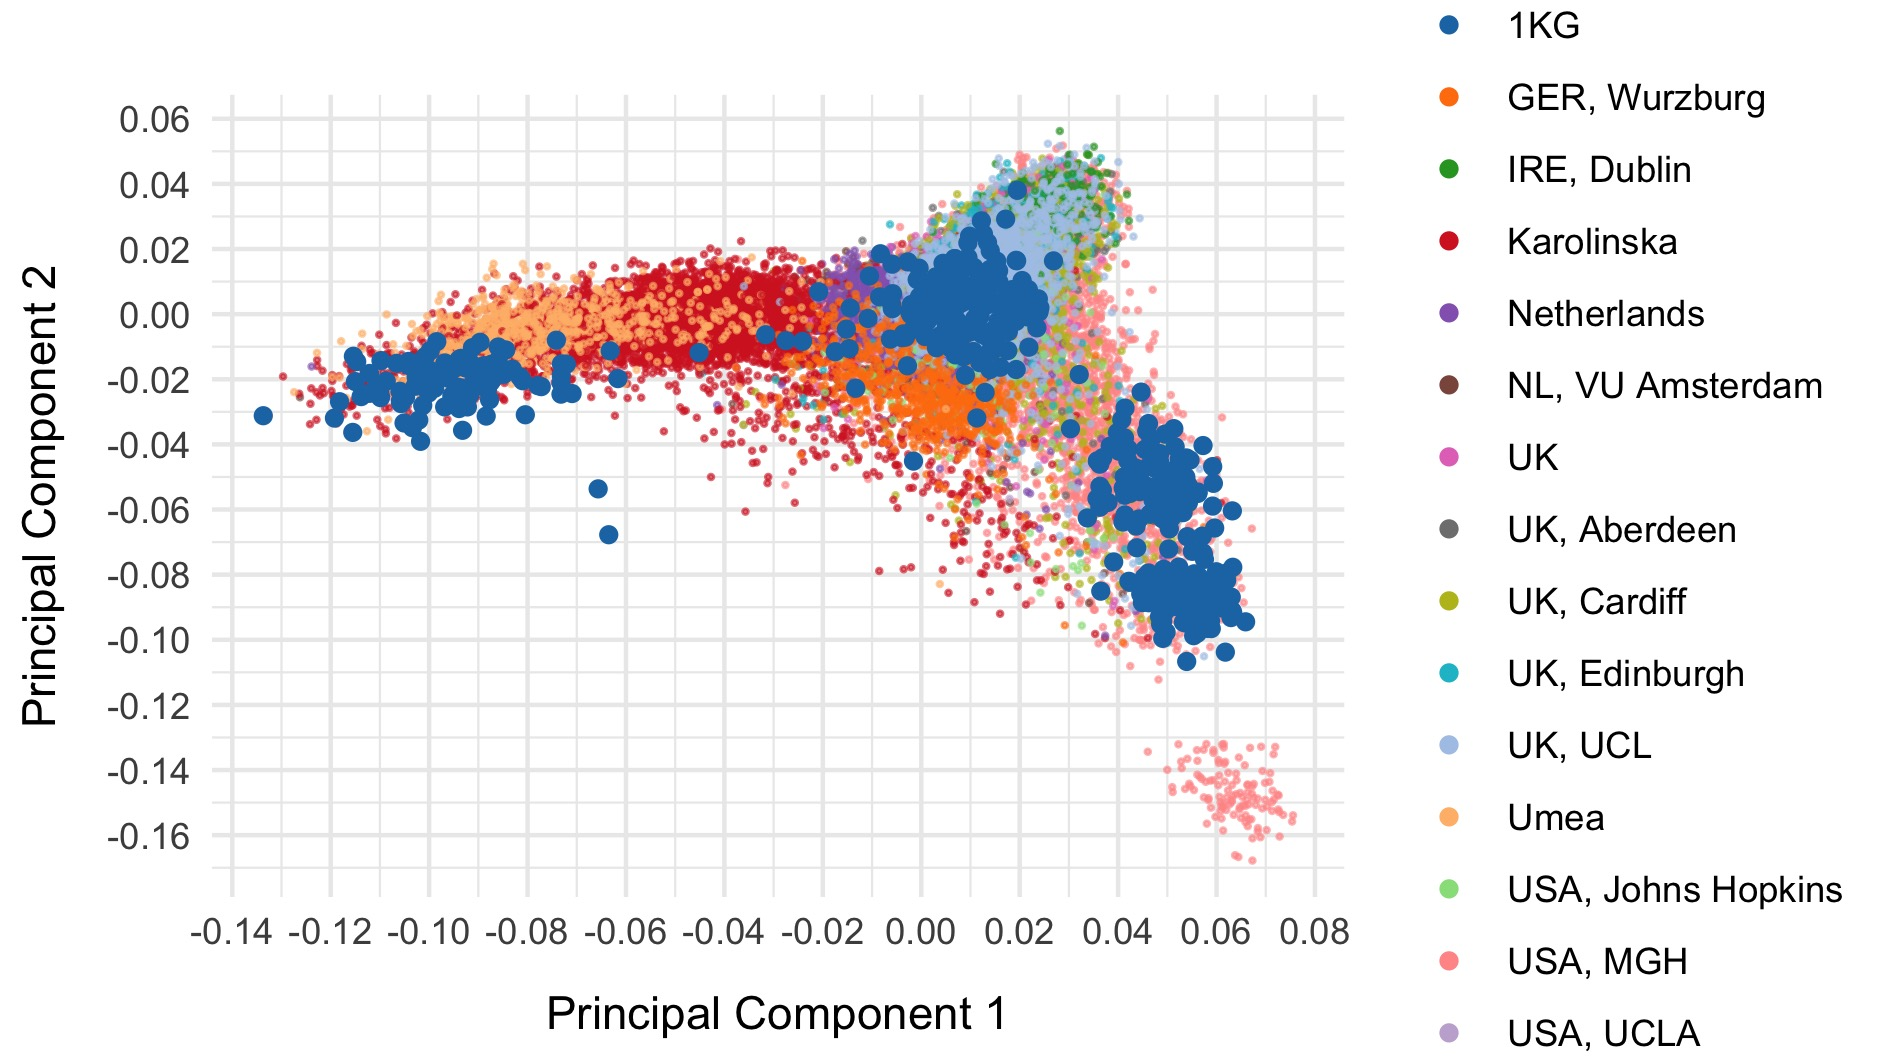
\includegraphics[width=0.5\textwidth]{13_PC1PC2_EUR_and_AJ_1kg_collection.jpg}}\\
\subfloat{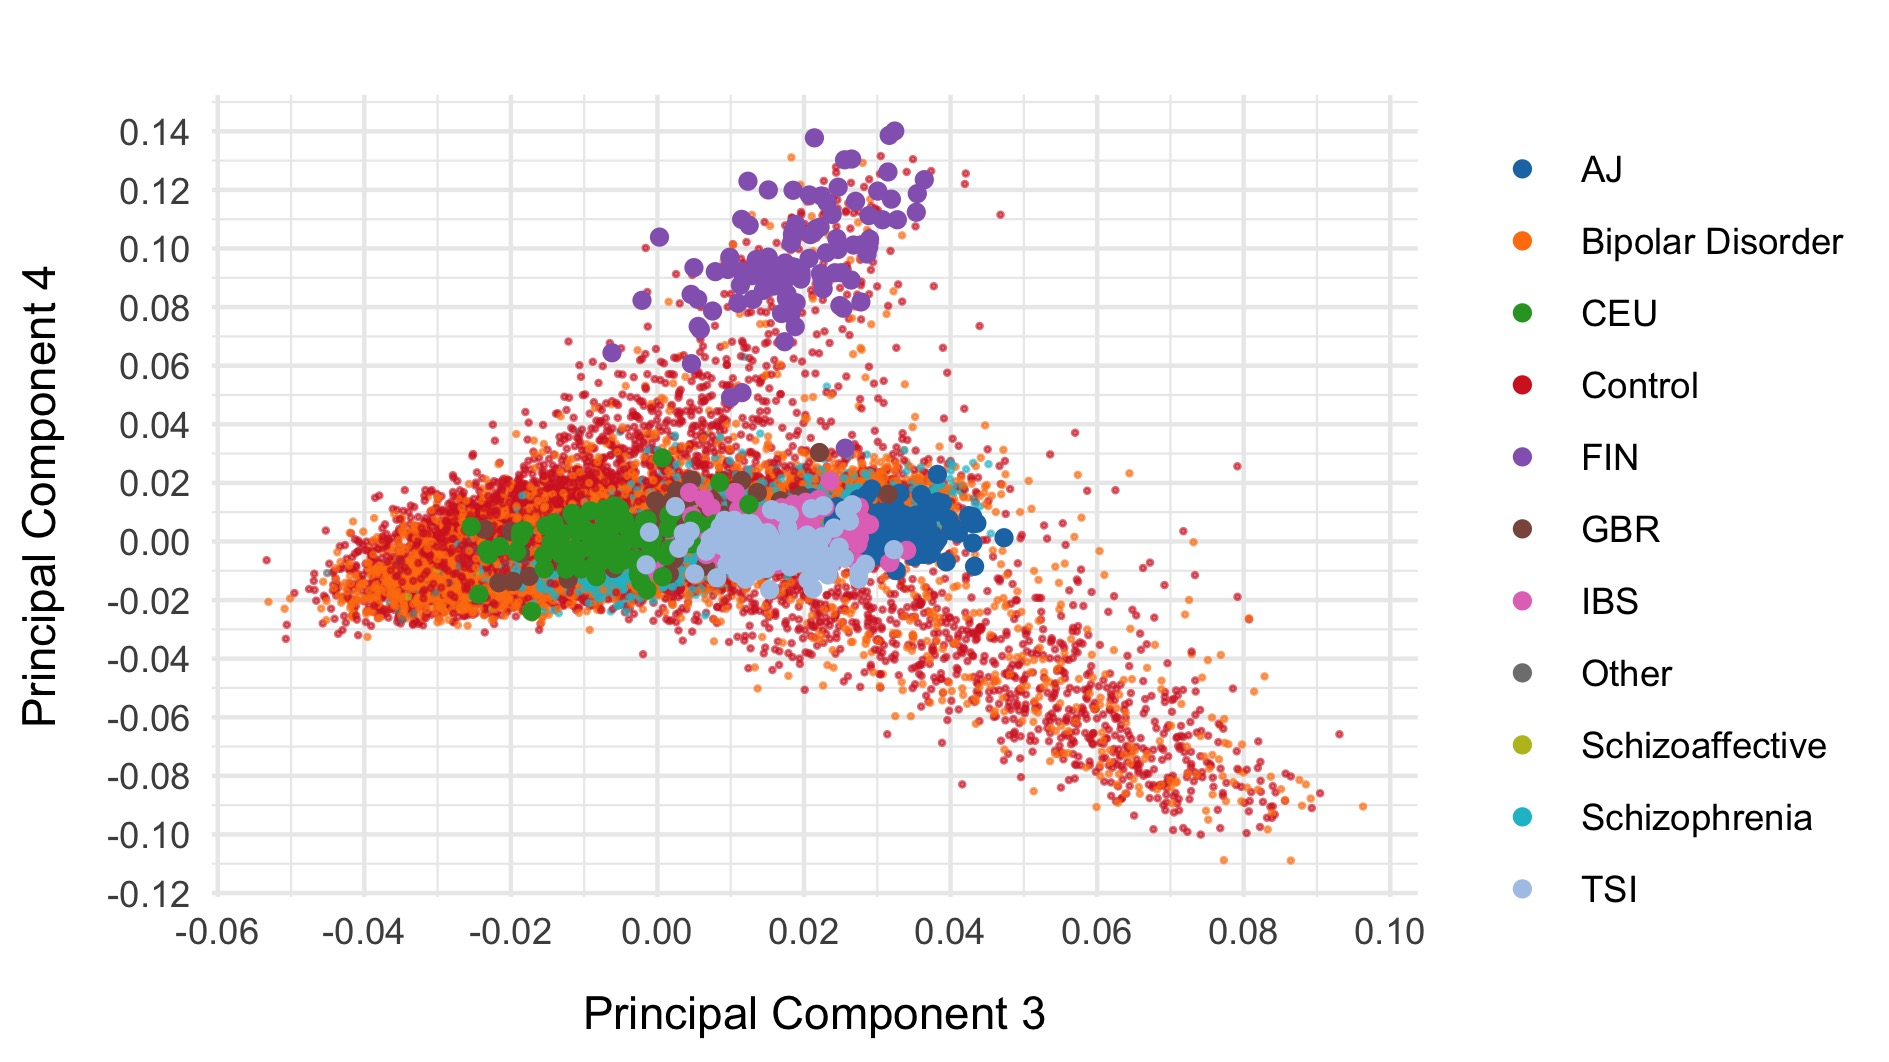
\includegraphics[width=0.5\textwidth]{13_PC3PC4_EUR_and_AJ_1kg.jpg}}
\subfloat{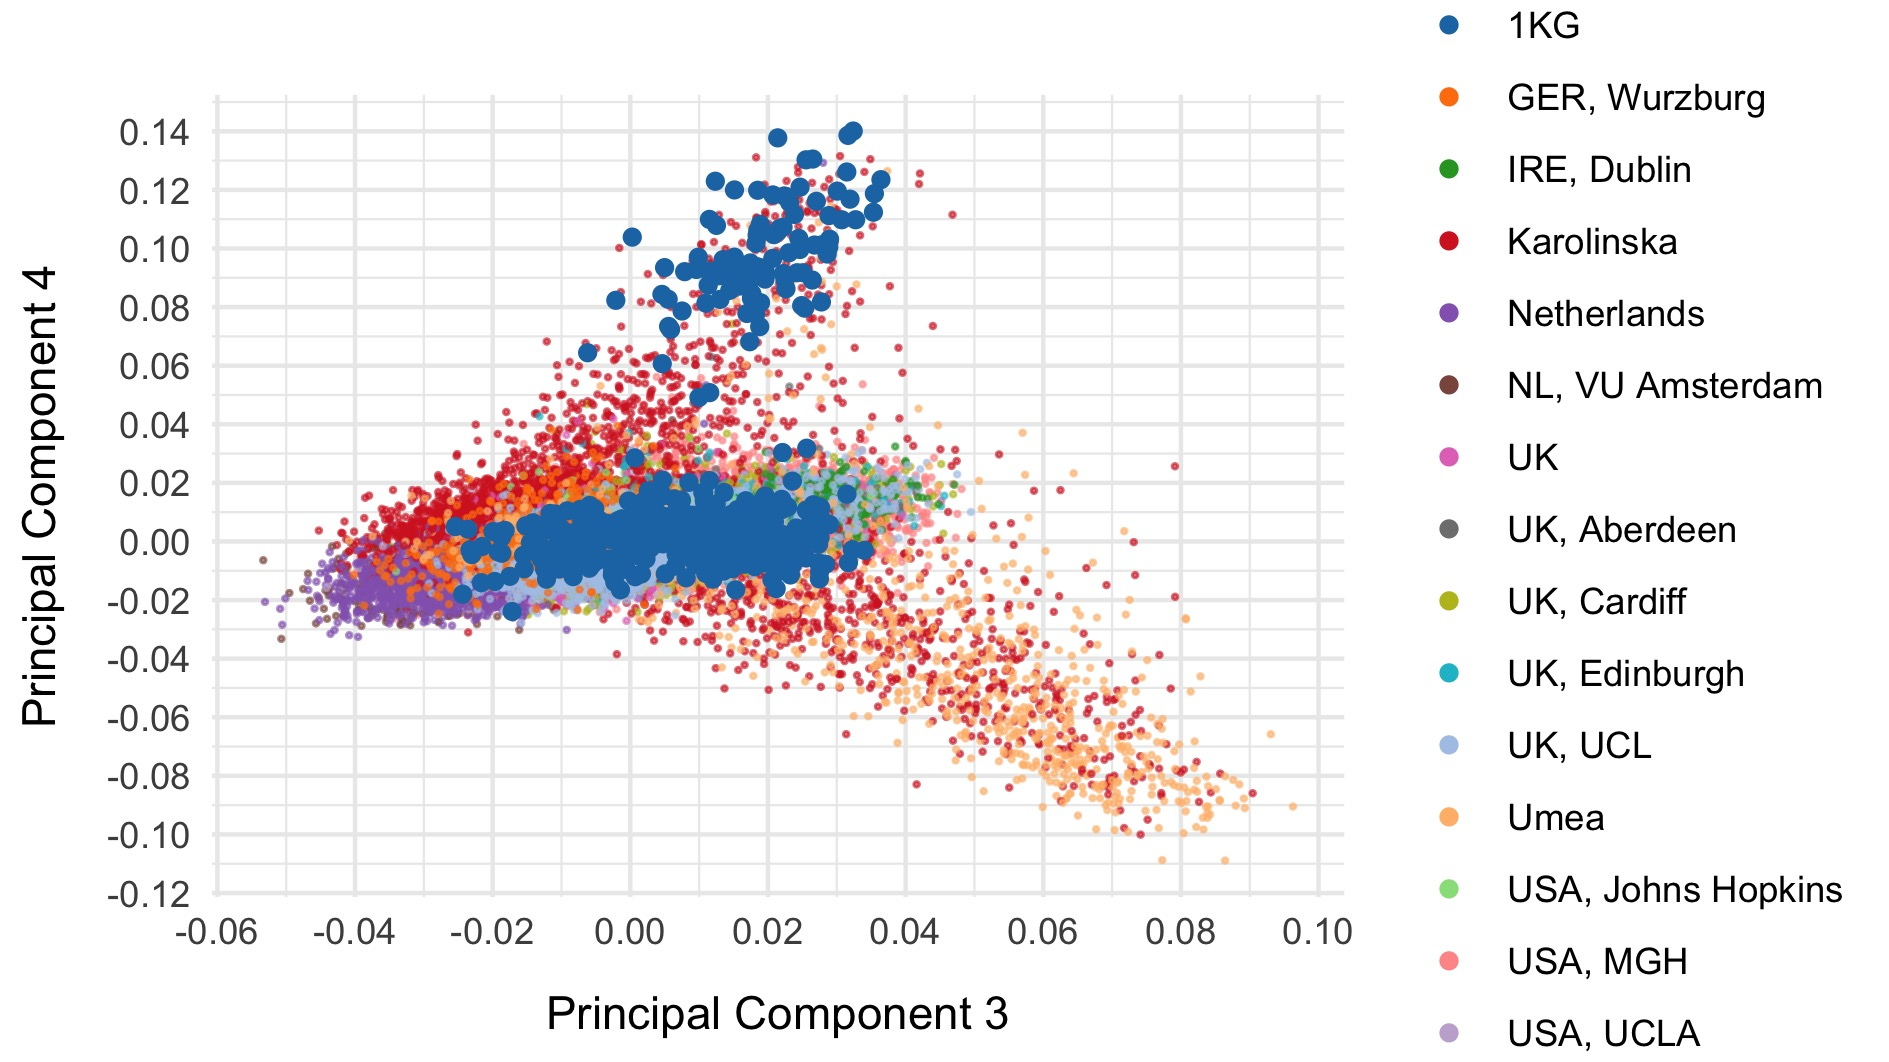
\includegraphics[width=0.5\textwidth]{13_PC3PC4_EUR_and_AJ_1kg_collection.jpg}}\\
\subfloat{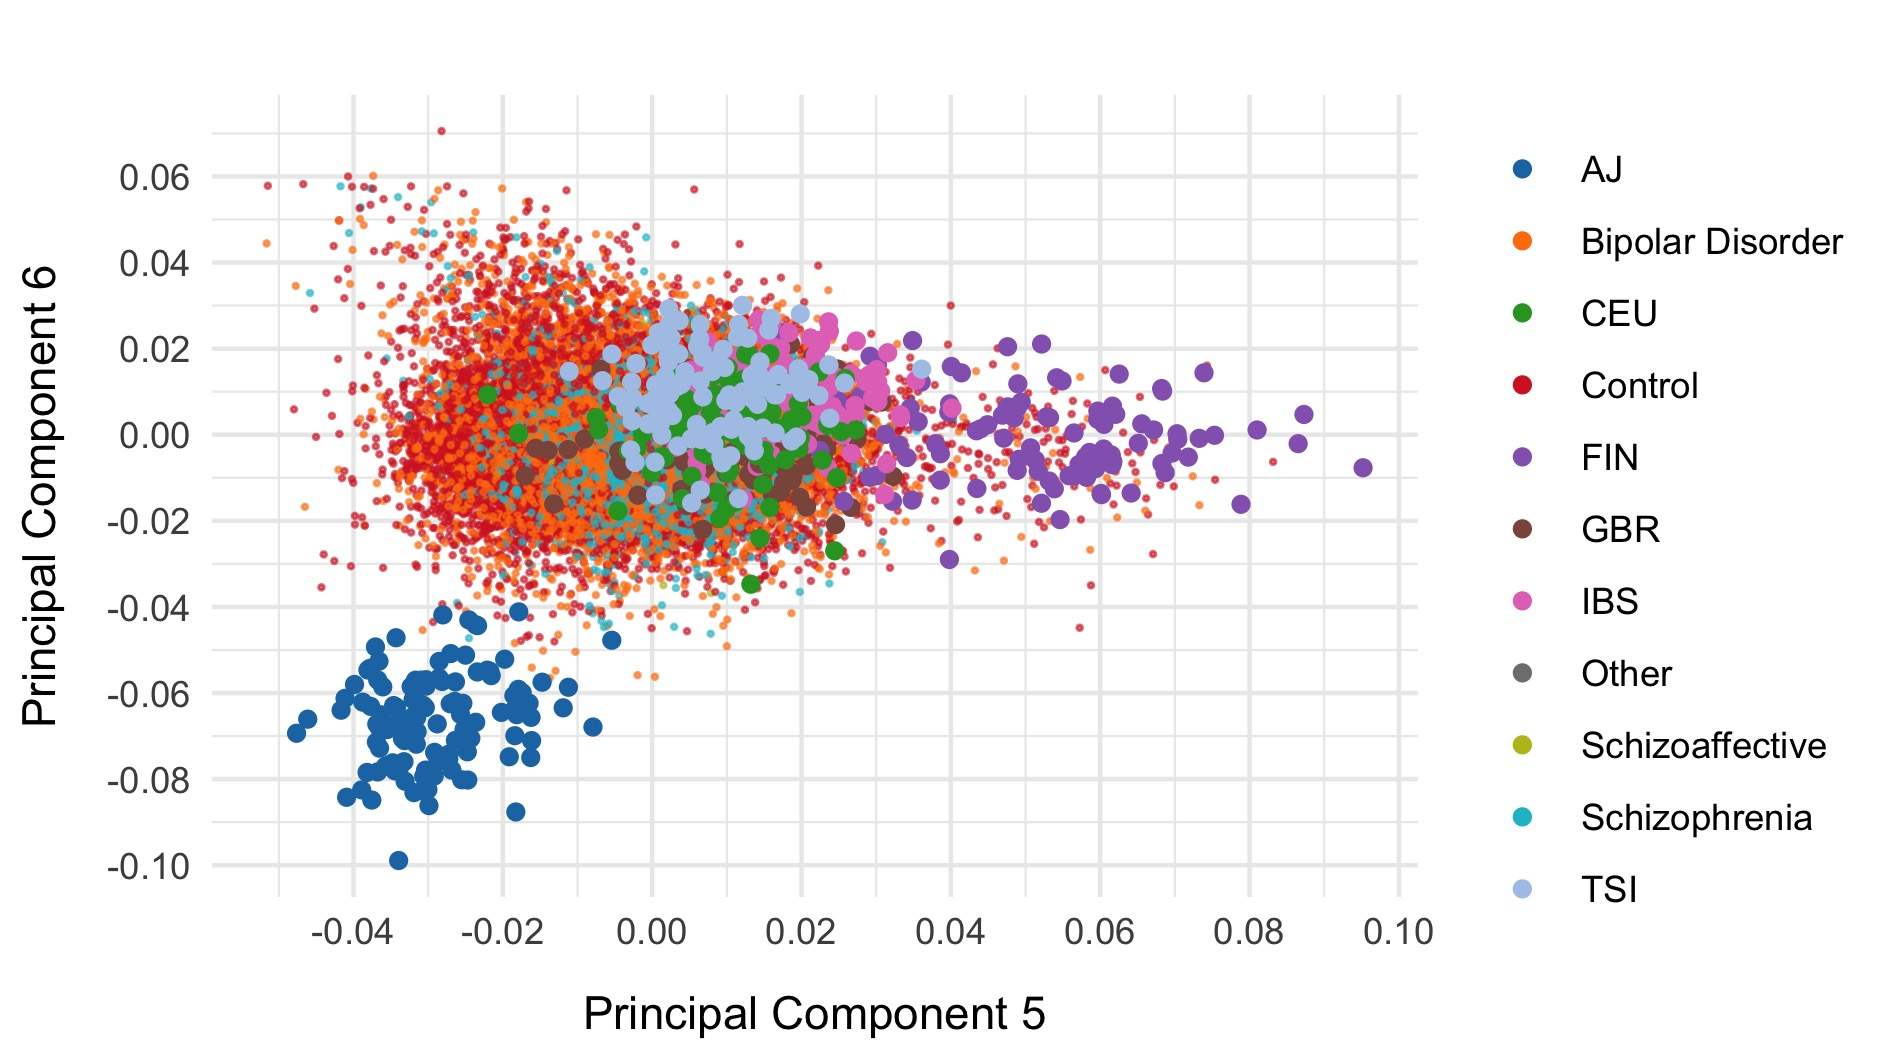
\includegraphics[width=0.5\textwidth]{13_PC5PC6_EUR_and_AJ_1kg.jpg}}
\subfloat{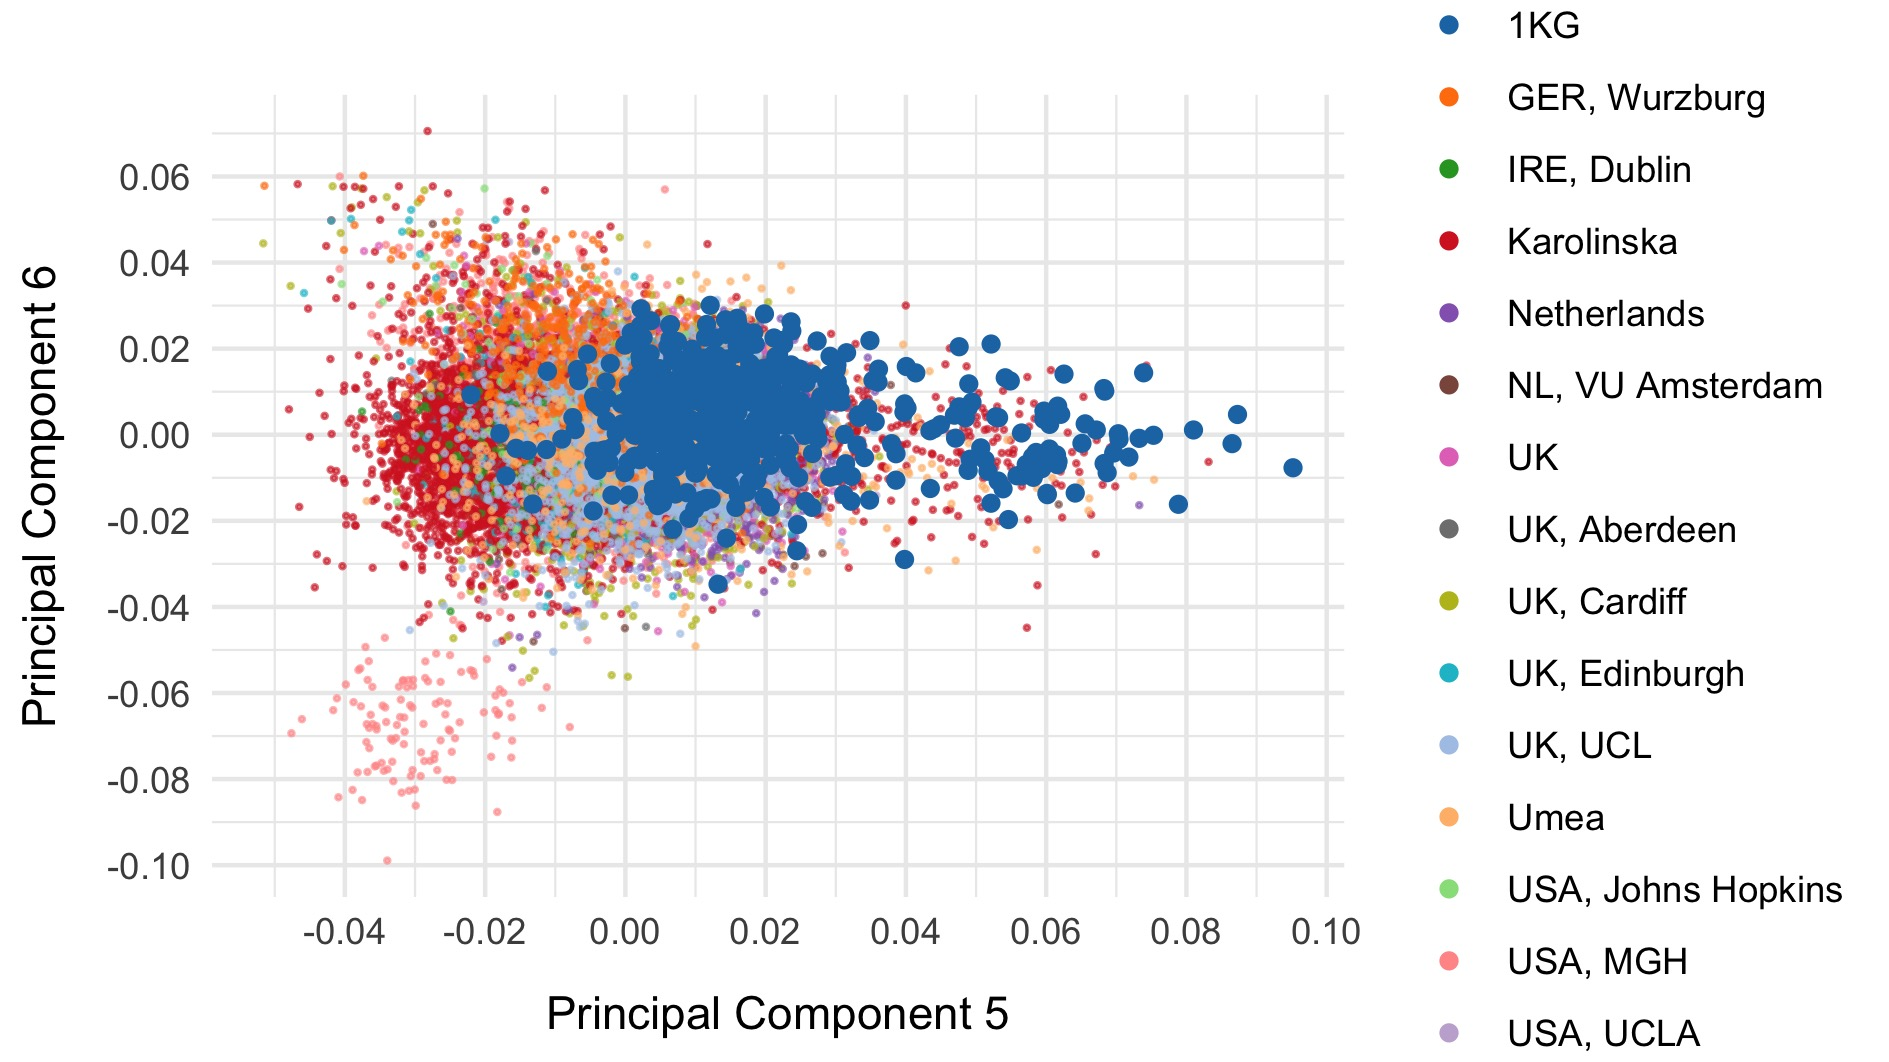
\includegraphics[width=0.5\textwidth]{13_PC5PC6_EUR_and_AJ_1kg_collection.jpg}}
\caption{PCA of European cohorts with 1000 Genomes}
\label{fig:PCA_EUR_AJ_1kg}
\end{figure}

% PCA 1kg EUR
\begin{figure}
\centering
\subfloat{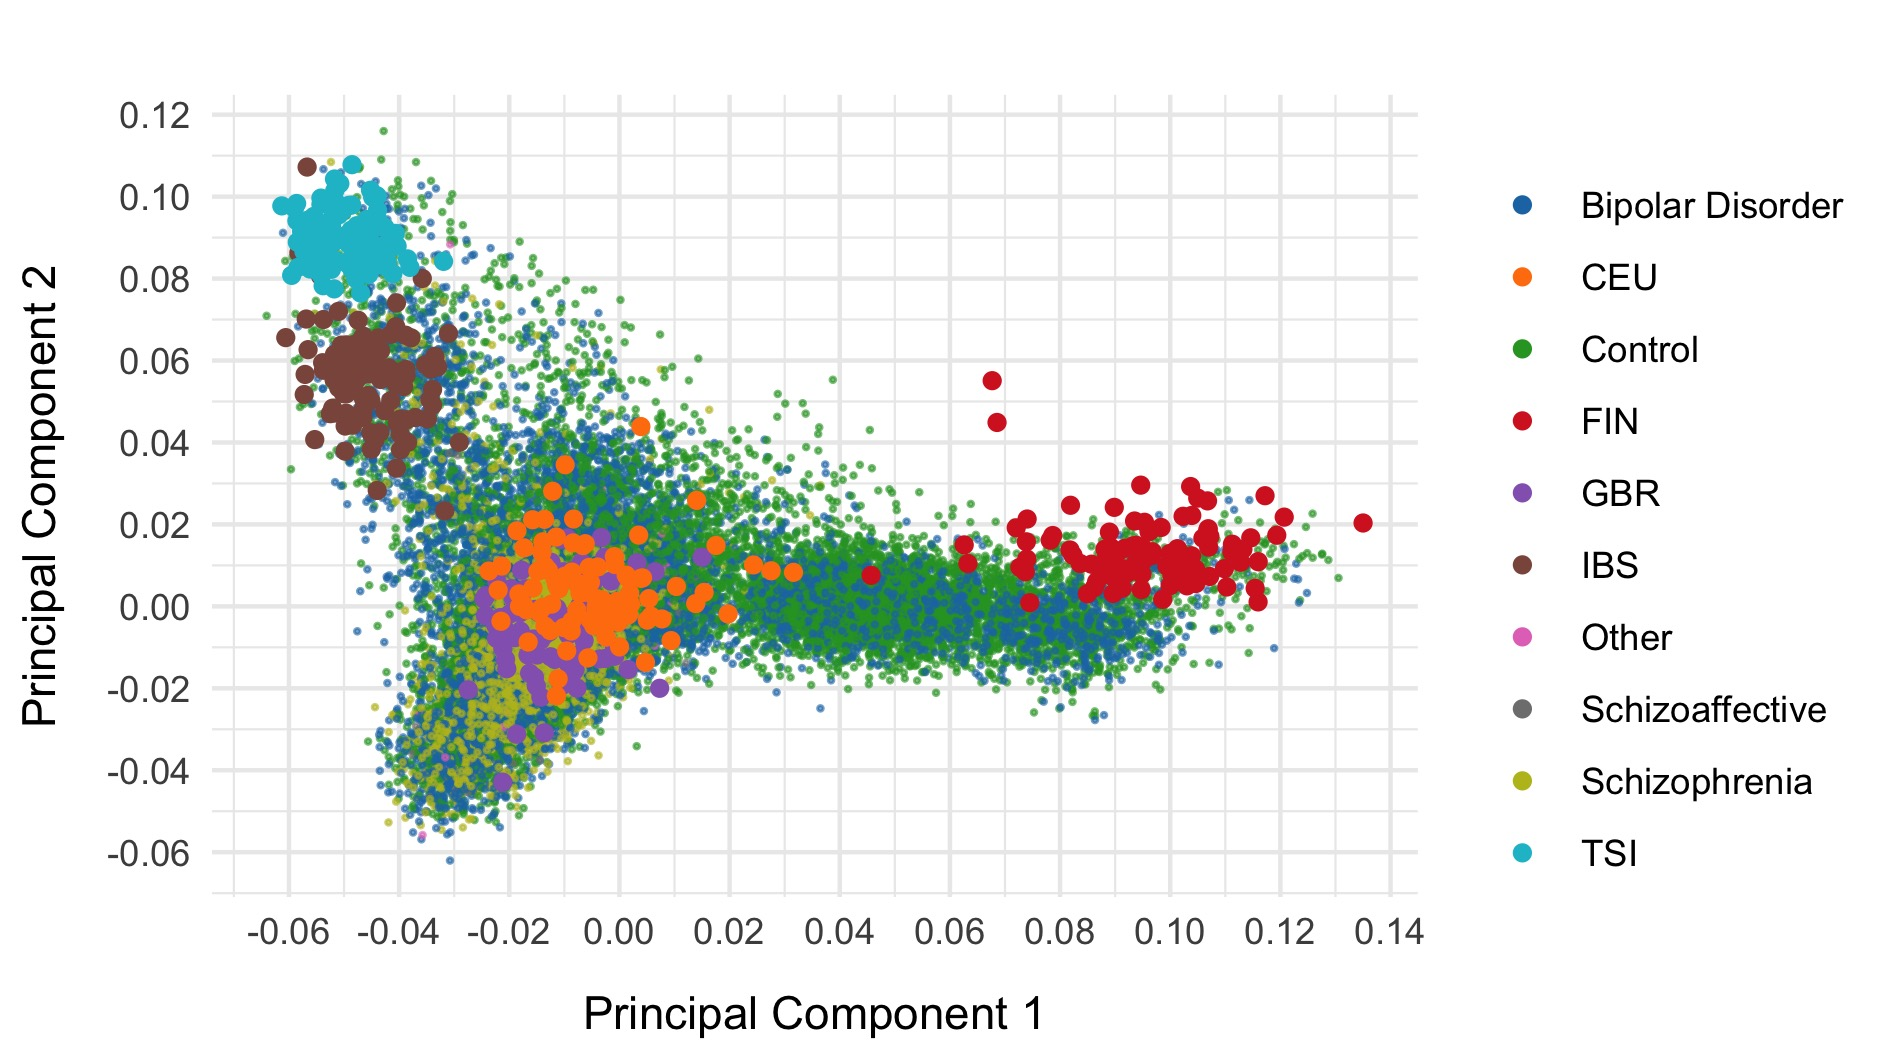
\includegraphics[width=0.5\textwidth]{13_PC1PC2_EUR_1kg.jpg}}
\subfloat{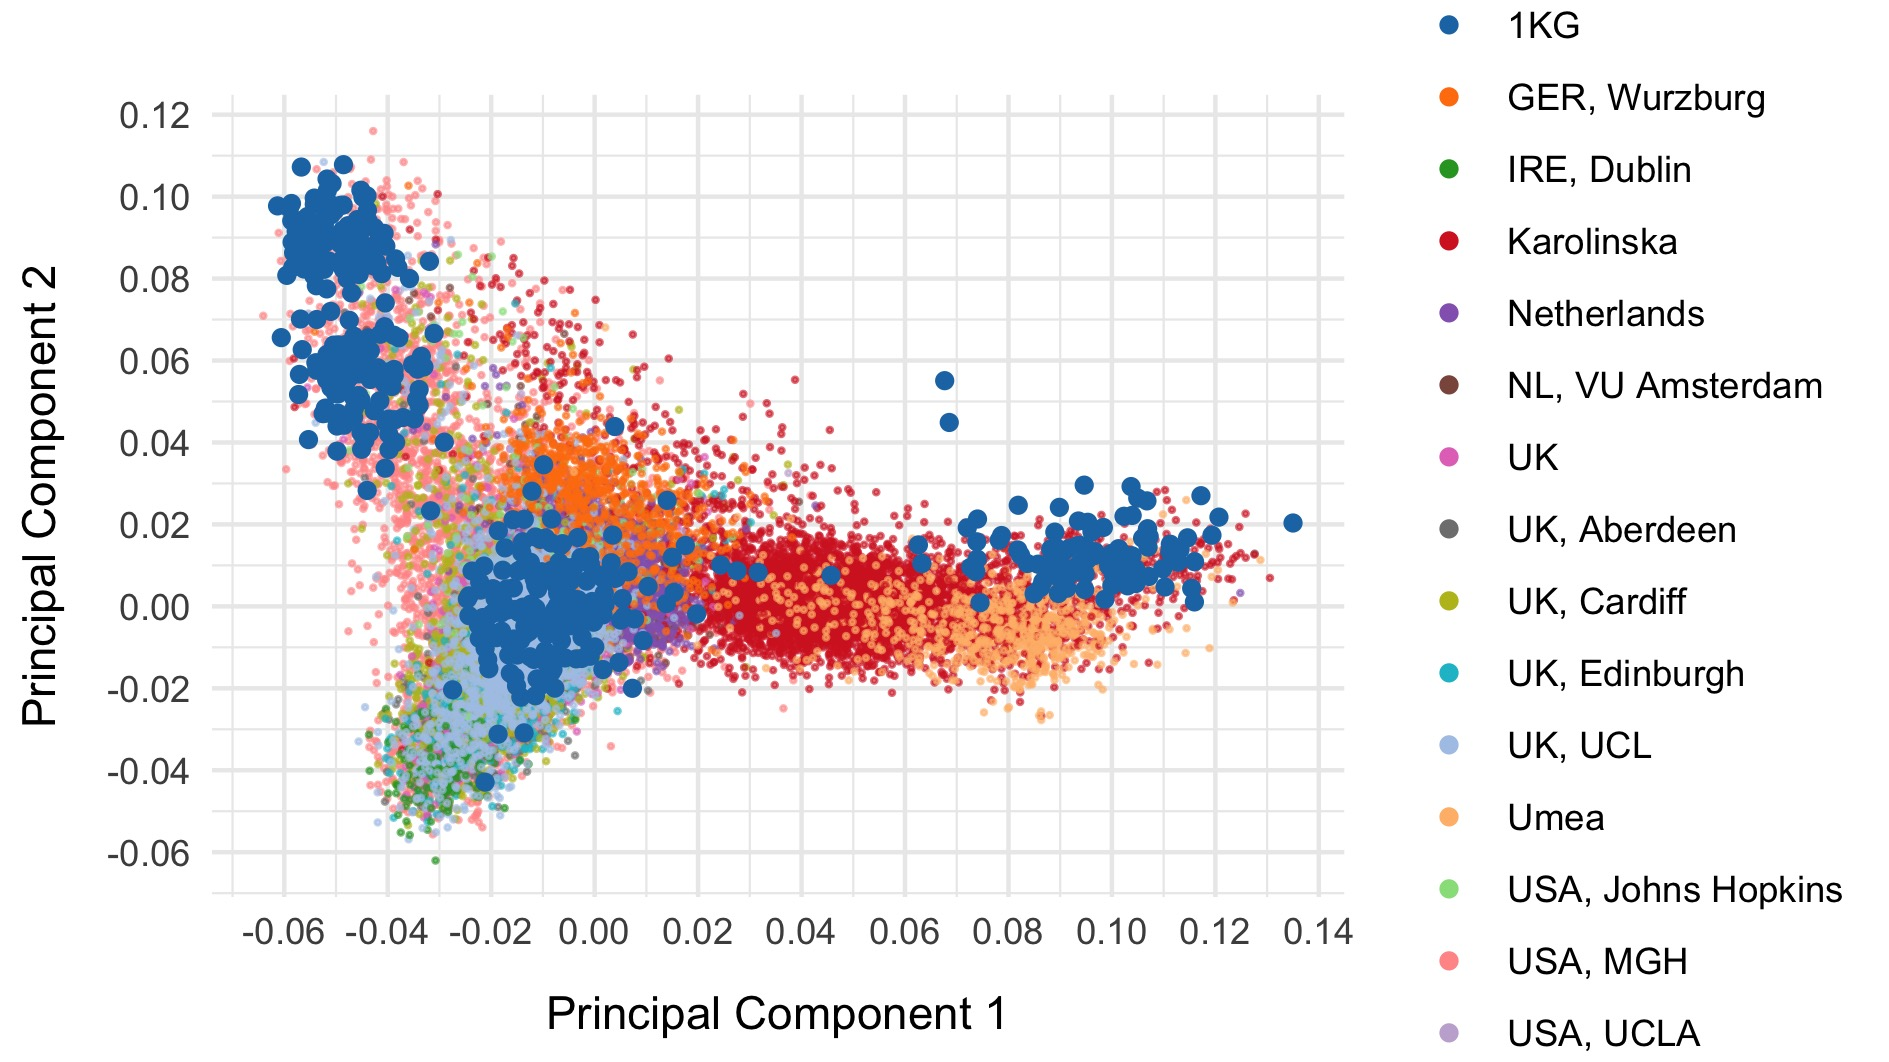
\includegraphics[width=0.5\textwidth]{13_PC1PC2_EUR_1kg_collection.jpg}}\\
\subfloat{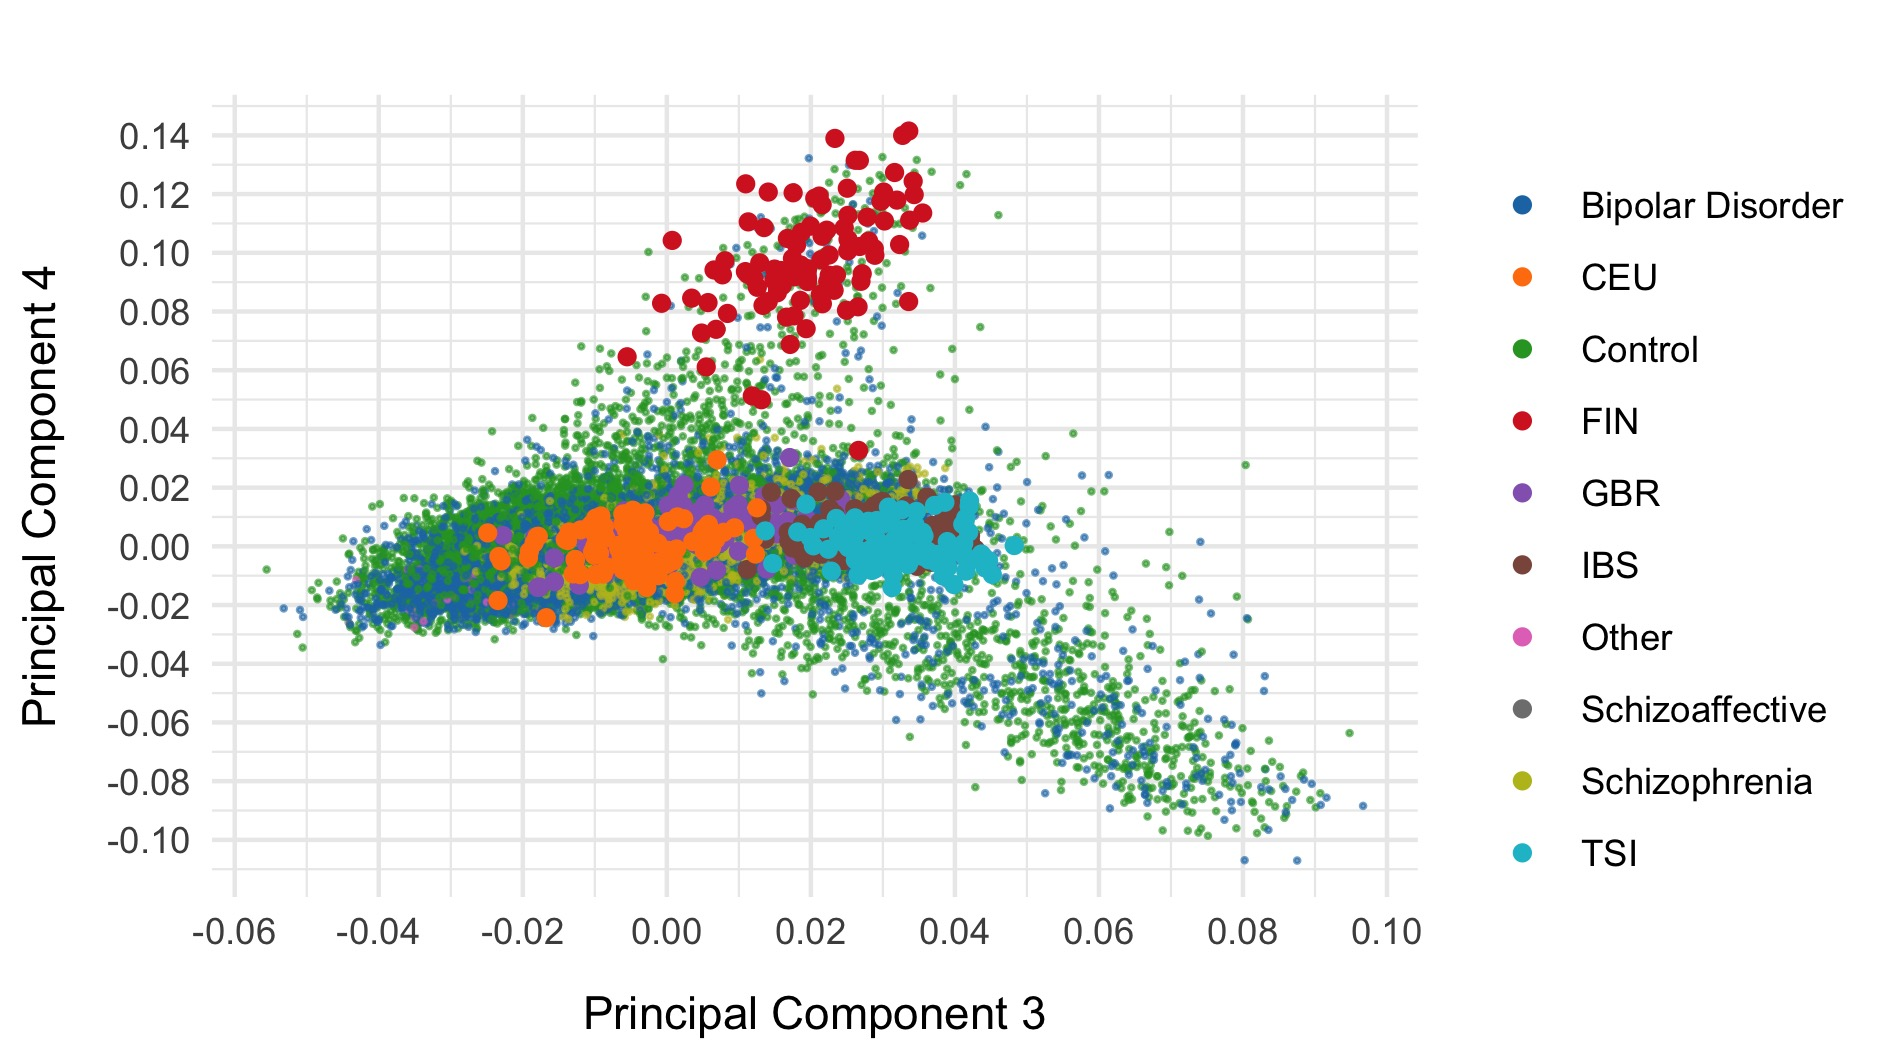
\includegraphics[width=0.5\textwidth]{13_PC3PC4_EUR_1kg.jpg}}
\subfloat{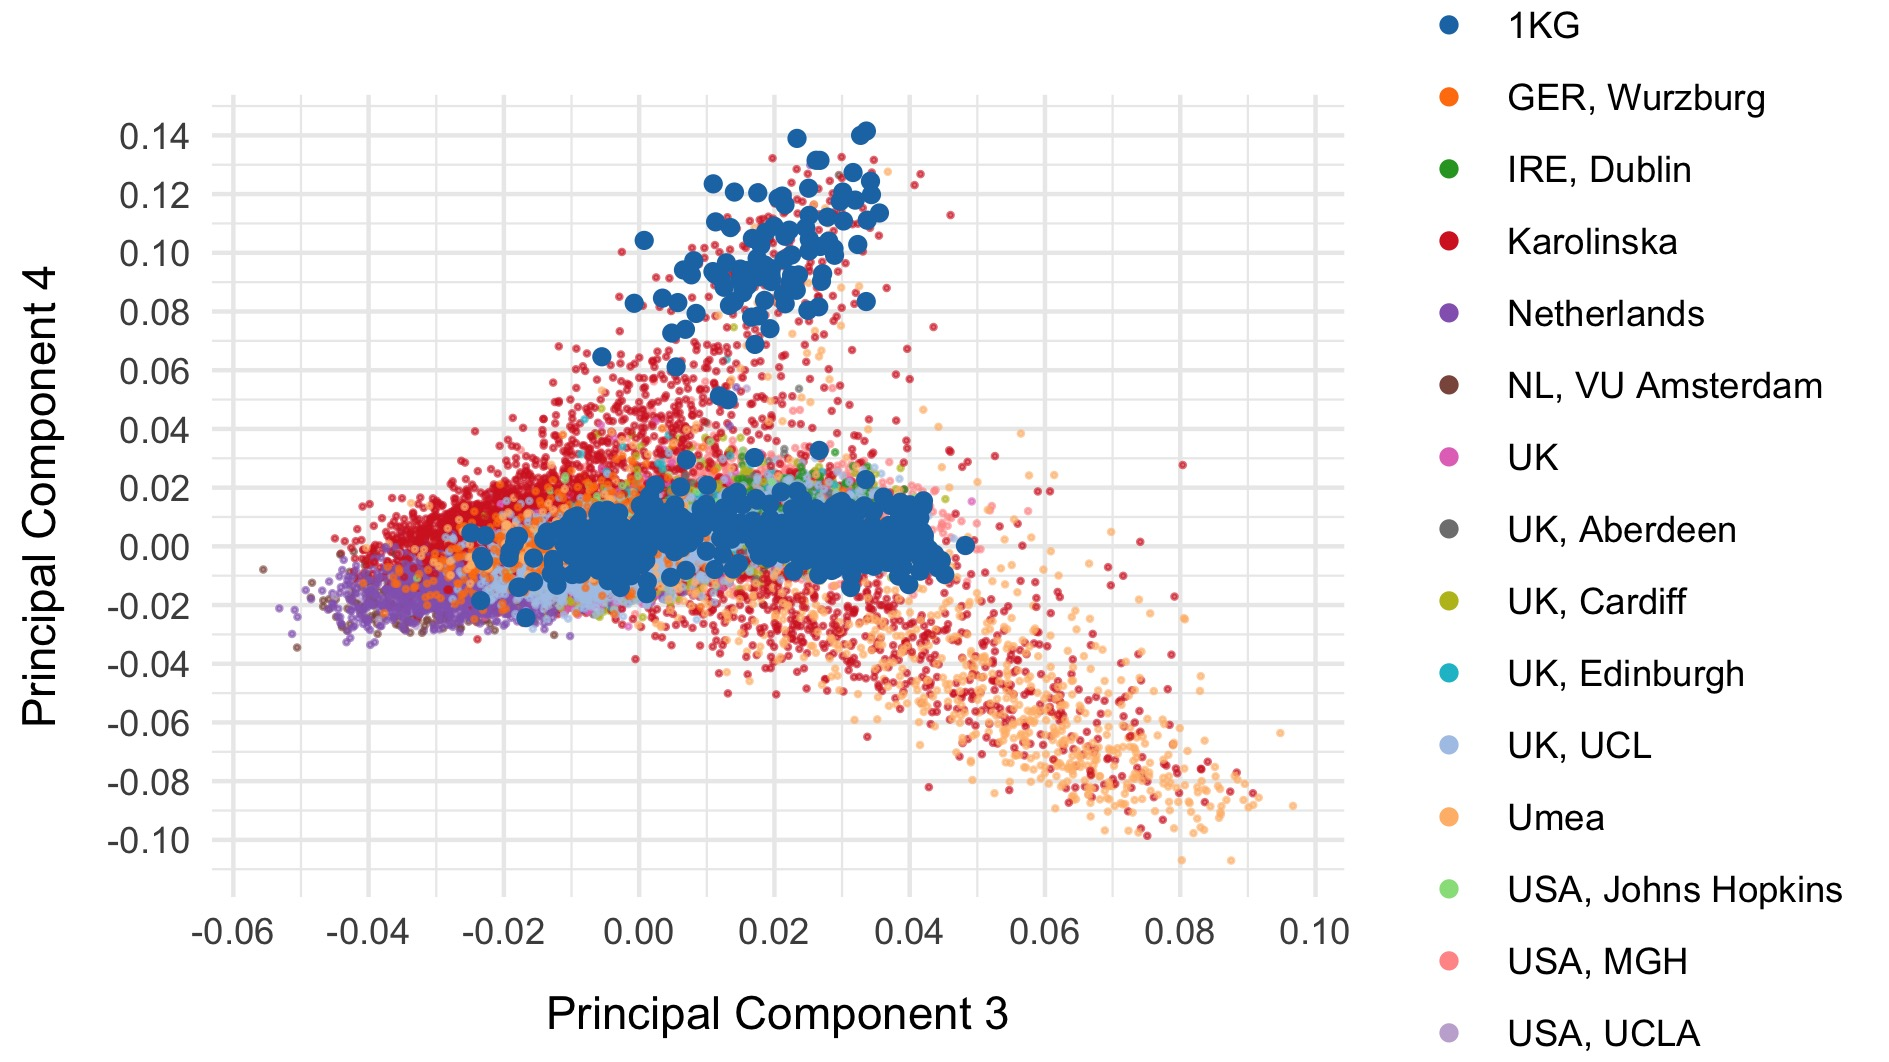
\includegraphics[width=0.5\textwidth]{13_PC3PC4_EUR_1kg_collection.jpg}}\\
\subfloat{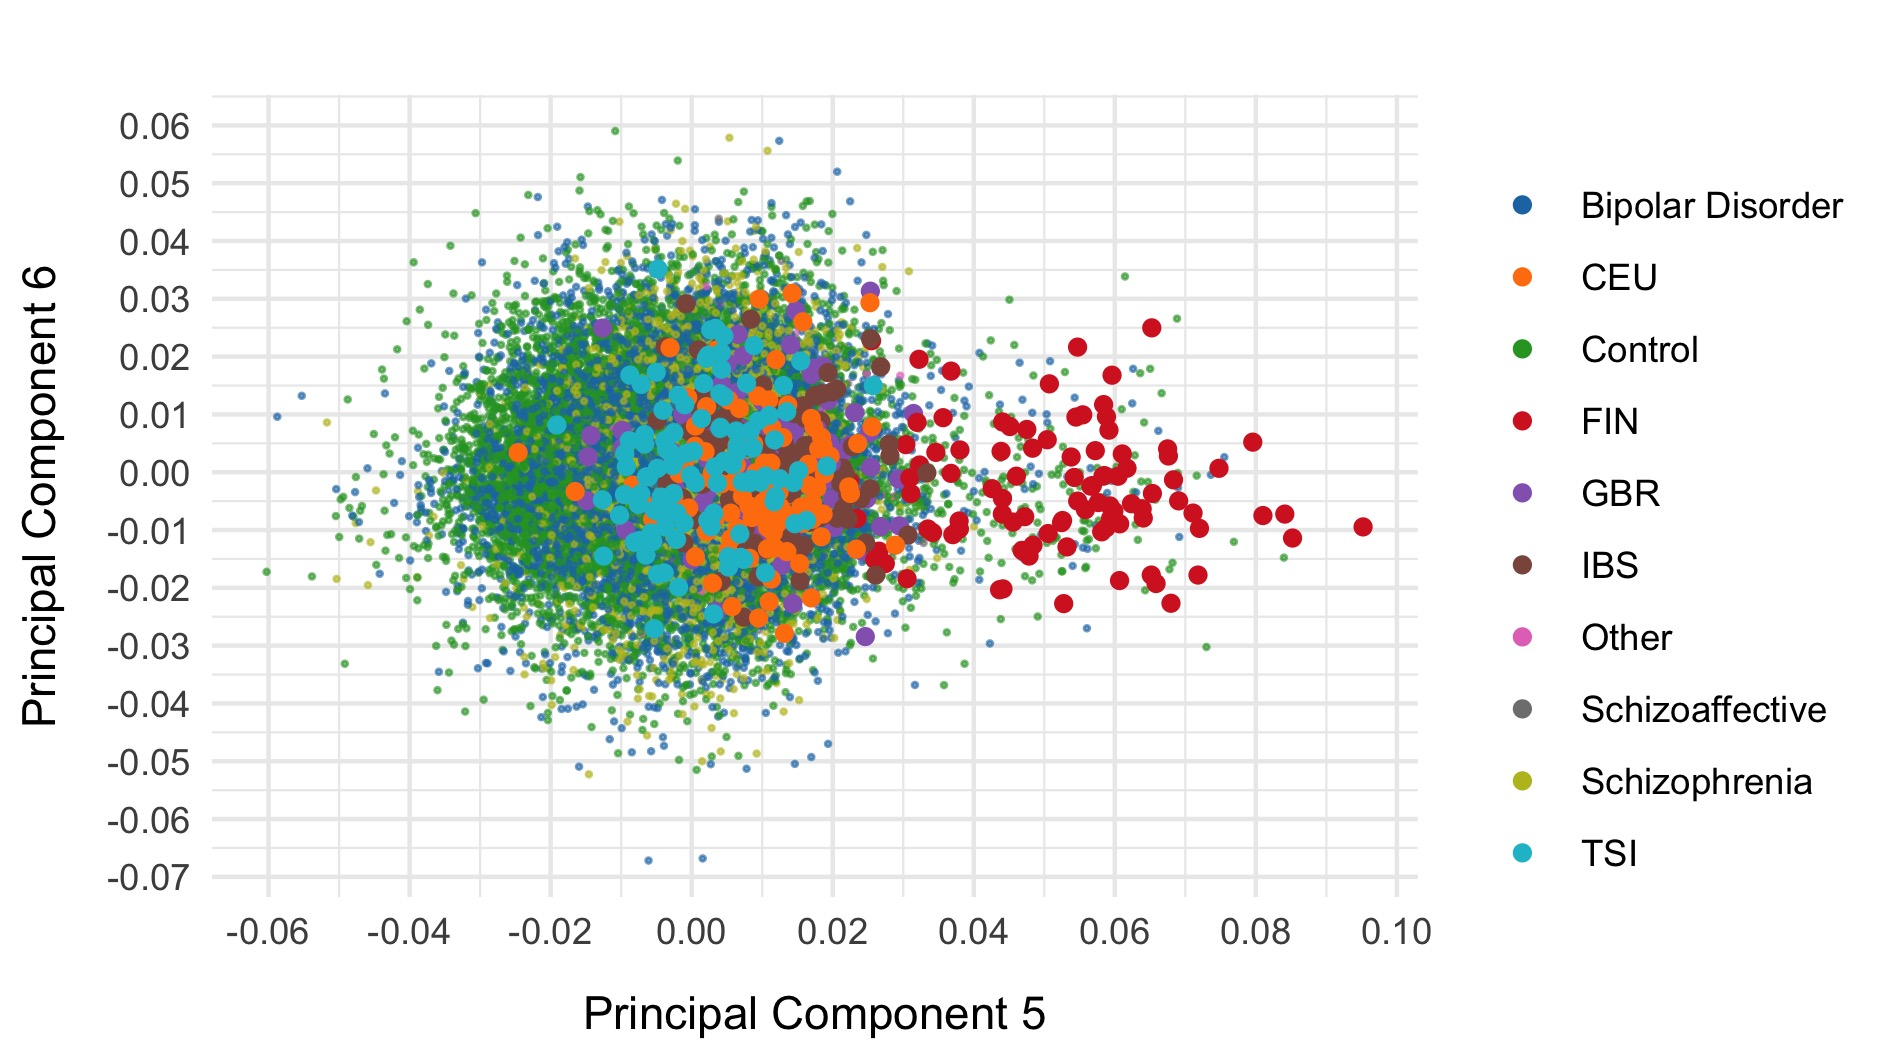
\includegraphics[width=0.5\textwidth]{13_PC5PC6_EUR_1kg.jpg}}
\subfloat{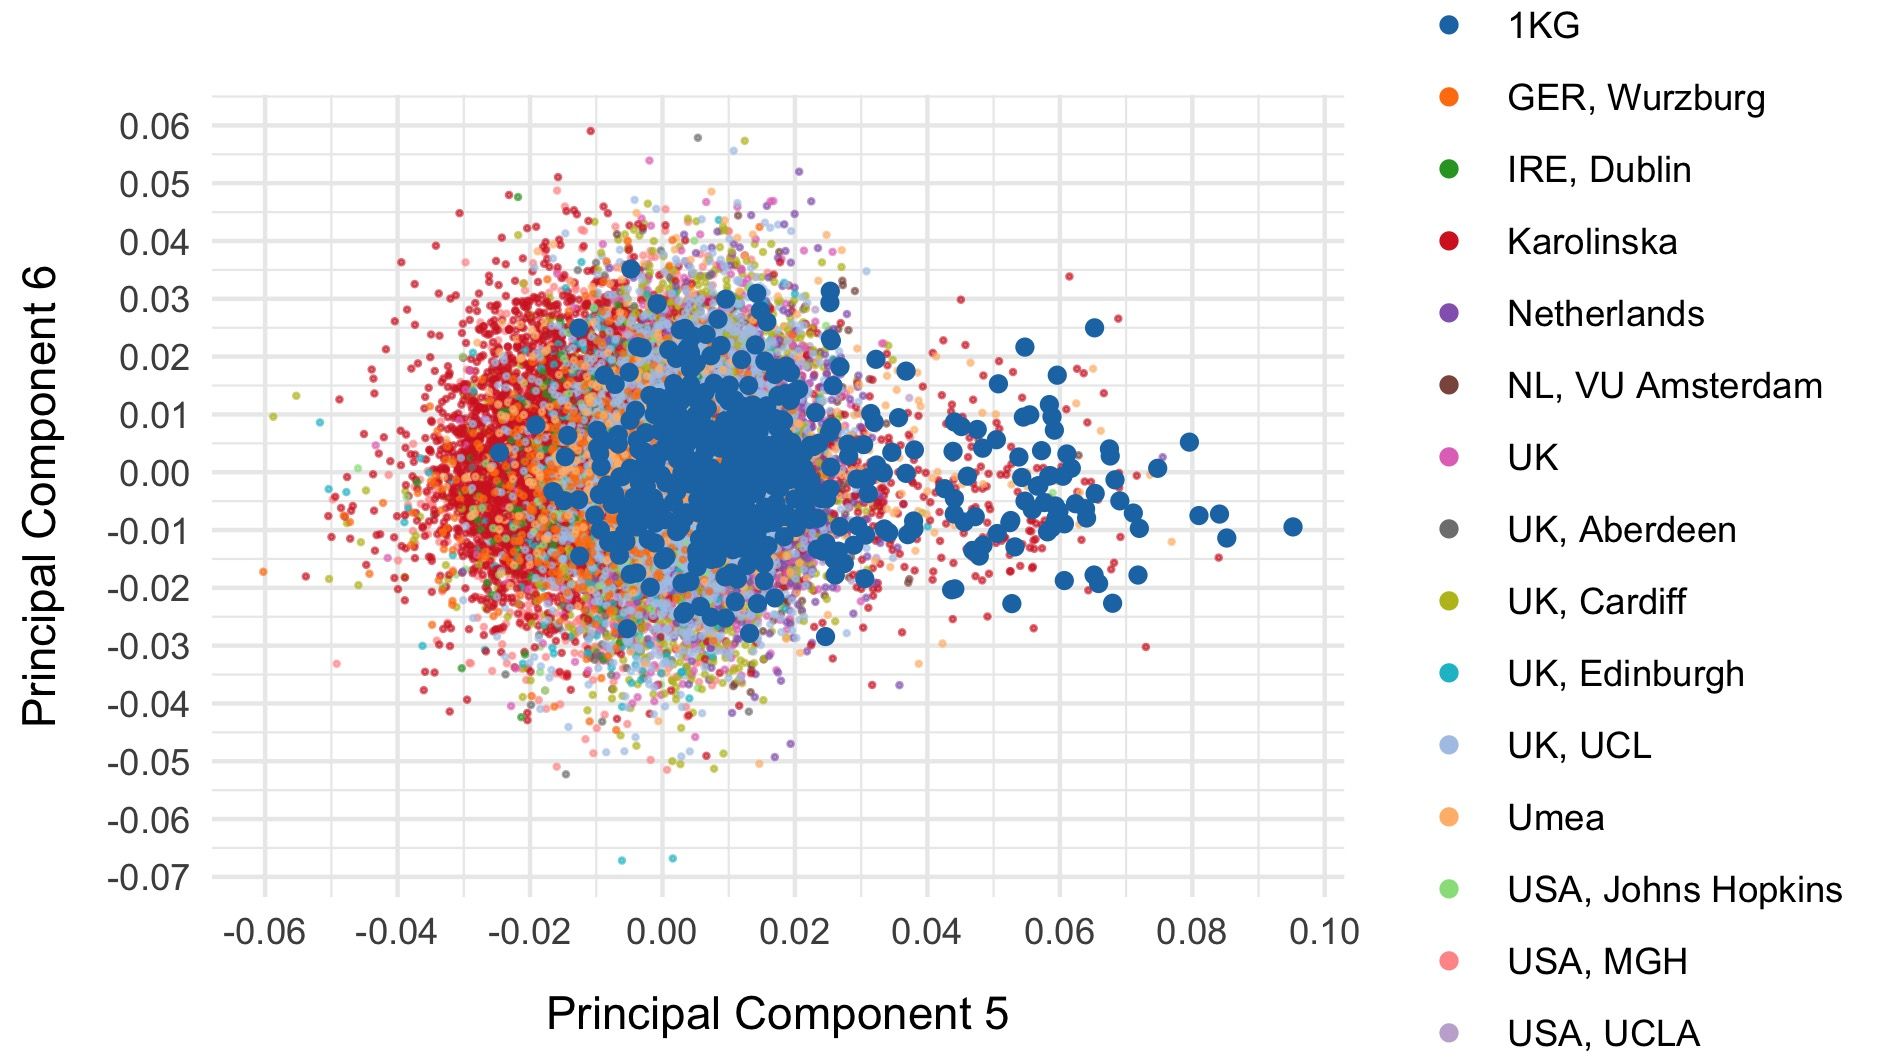
\includegraphics[width=0.5\textwidth]{13_PC5PC6_EUR_1kg_collection.jpg}}
\caption{PCA of European cohorts with 1000 Genomes}
\label{fig:PCA_EUR_1kg}
\end{figure}

% PCA 1kg mainland EUR
\begin{figure}
\centering
\subfloat{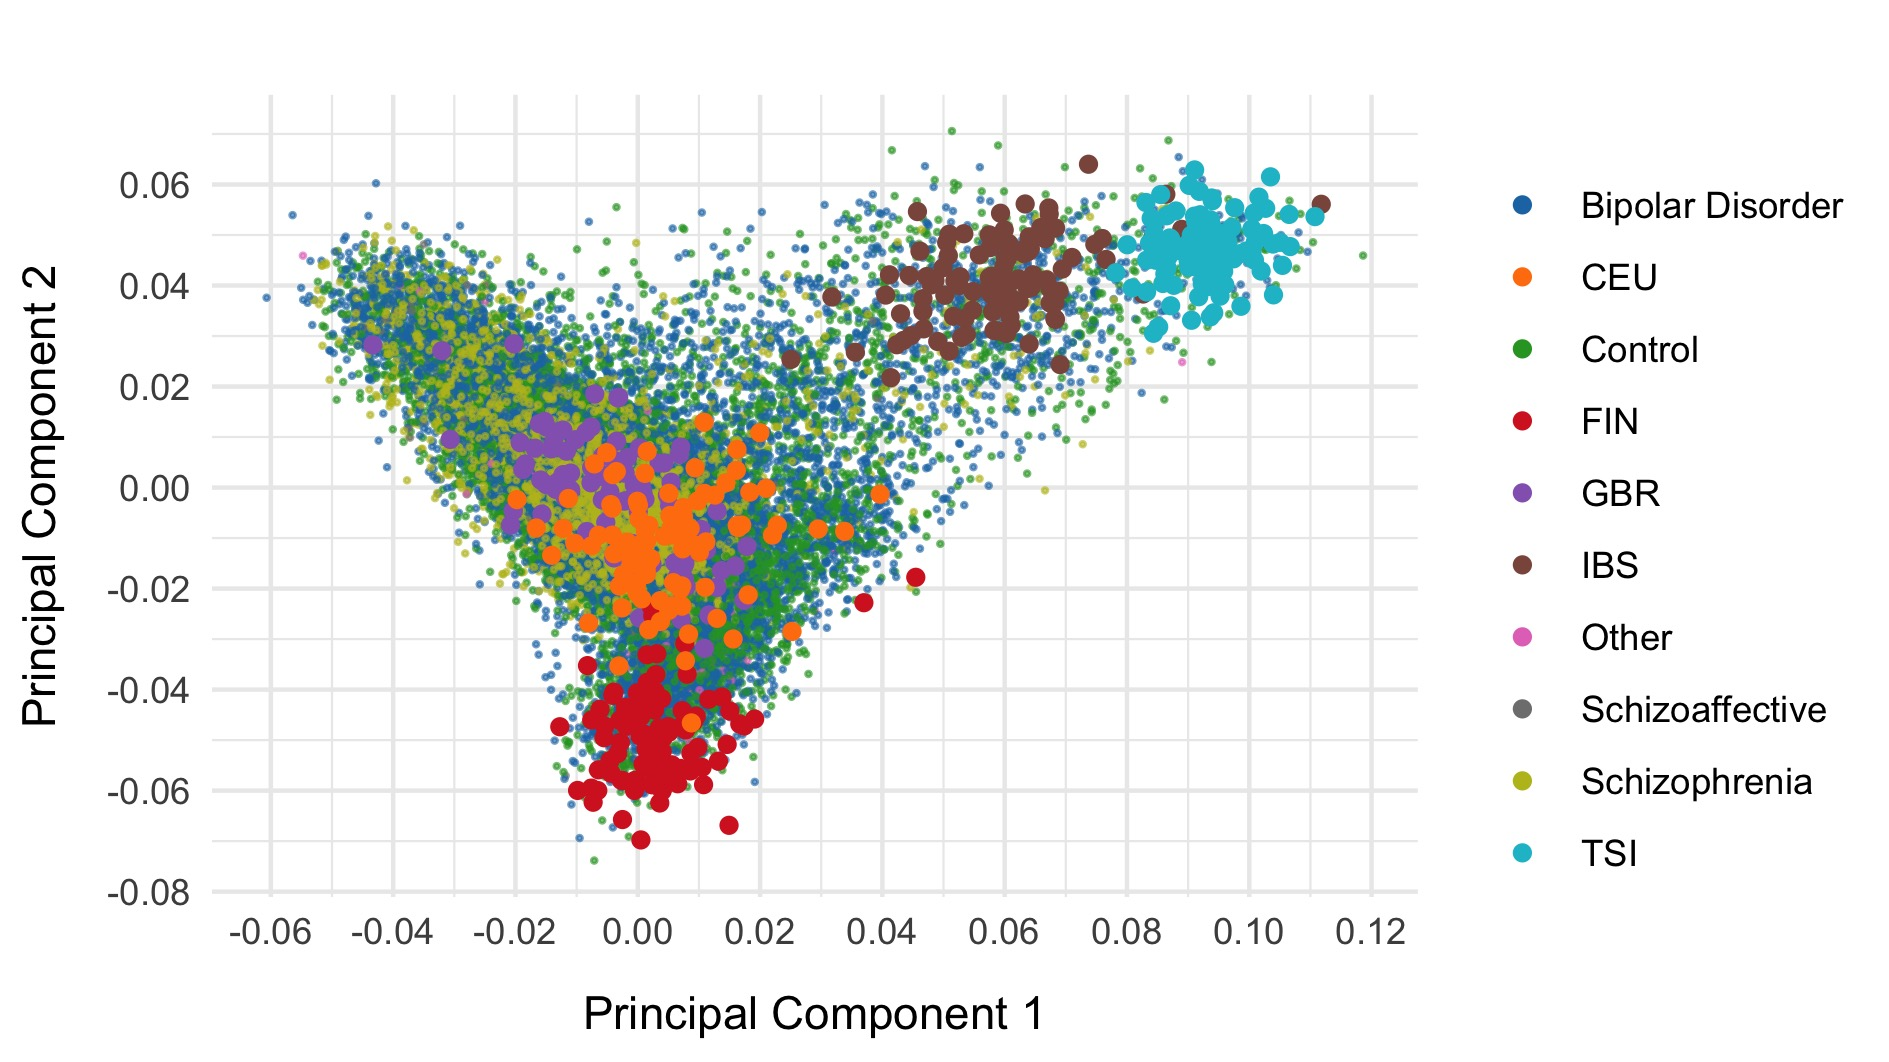
\includegraphics[width=0.5\textwidth]{13_PC1PC2_mainland_EUR_1kg.jpg}}
\subfloat{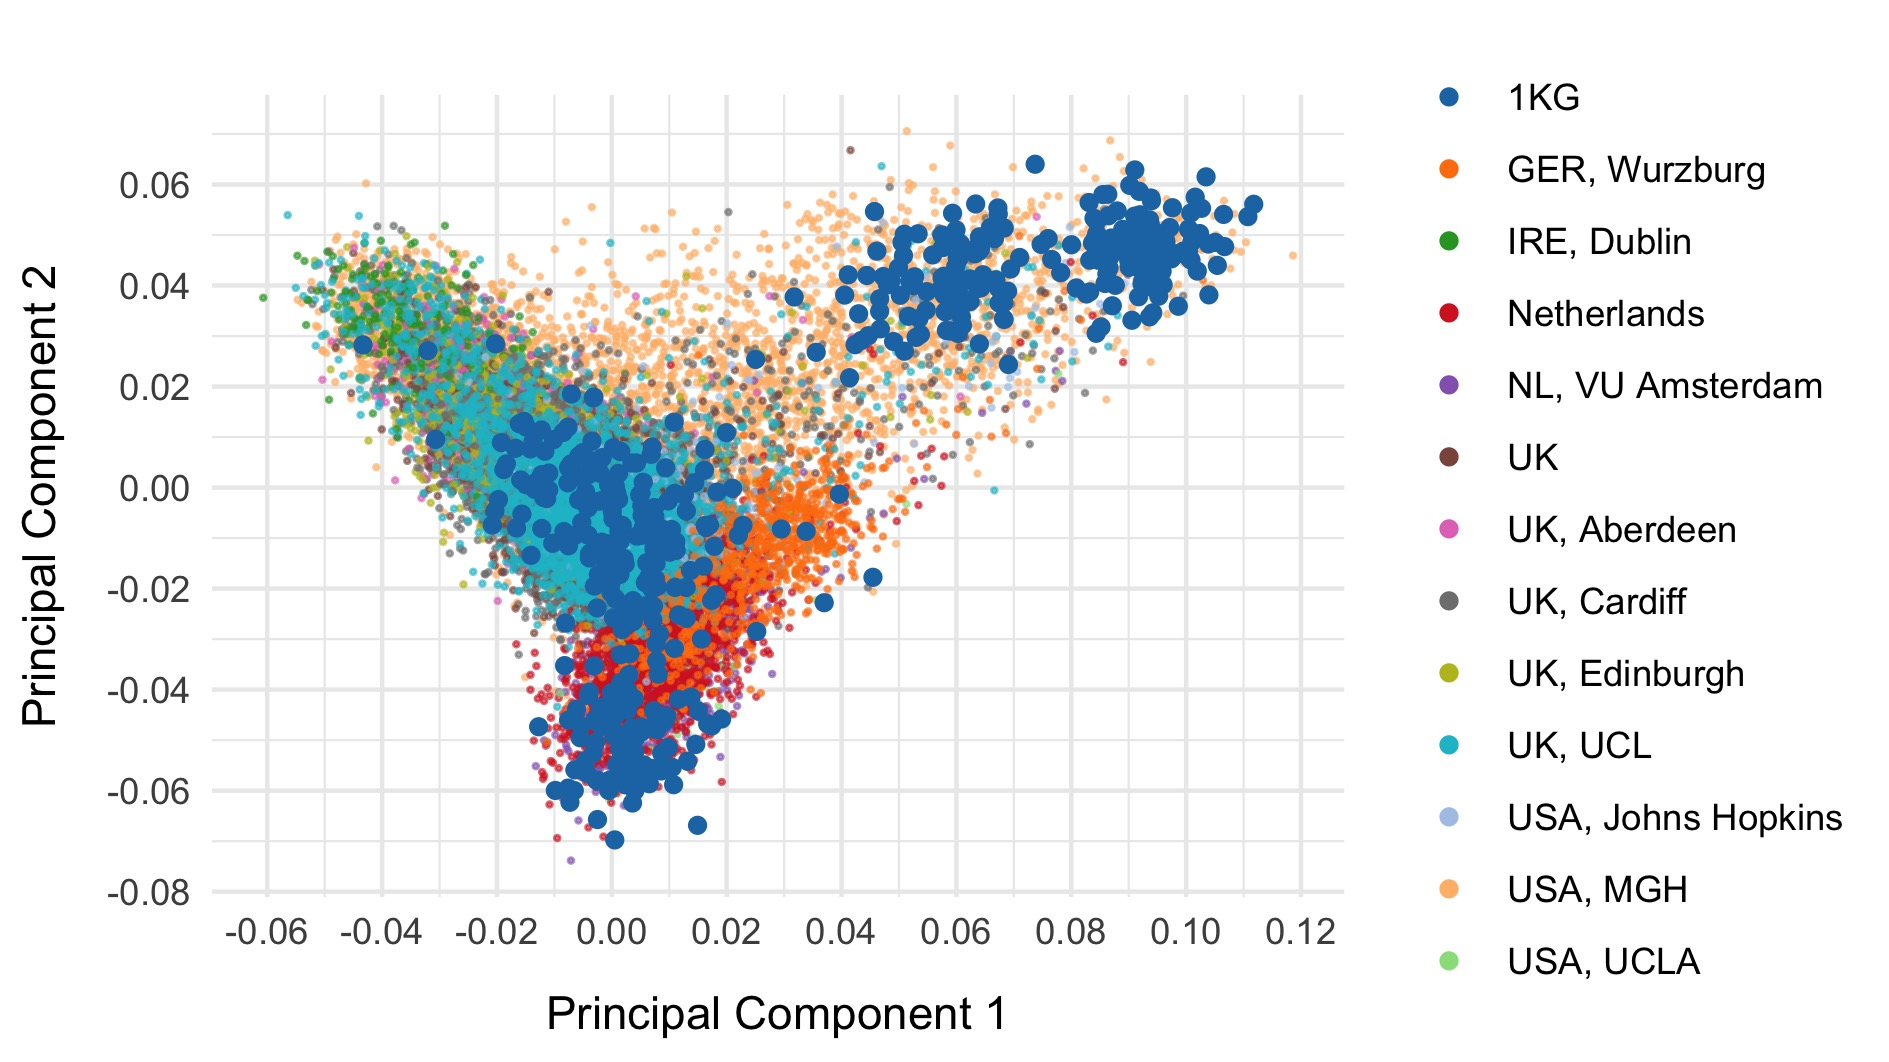
\includegraphics[width=0.5\textwidth]{13_PC1PC2_mainland_EUR_1kg_collection.jpg}}\\
\subfloat{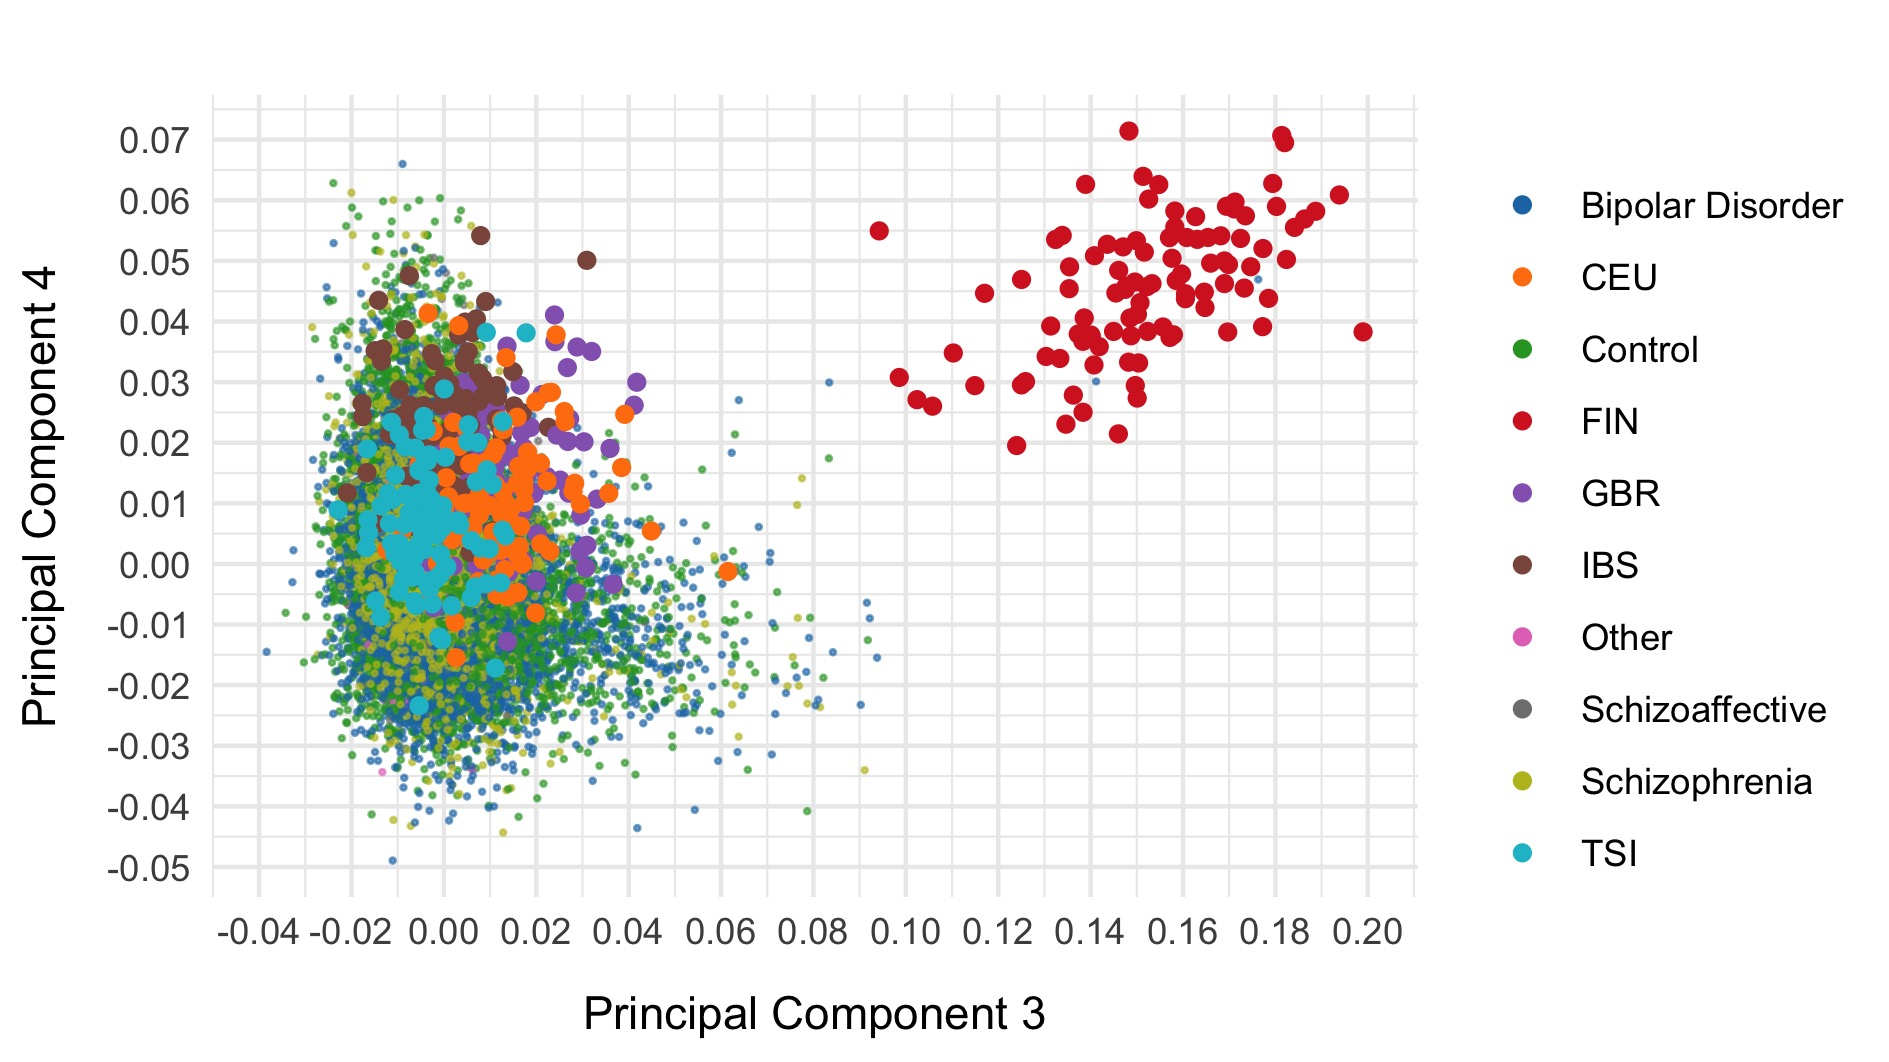
\includegraphics[width=0.5\textwidth]{13_PC3PC4_mainland_EUR_1kg.jpg}}
\subfloat{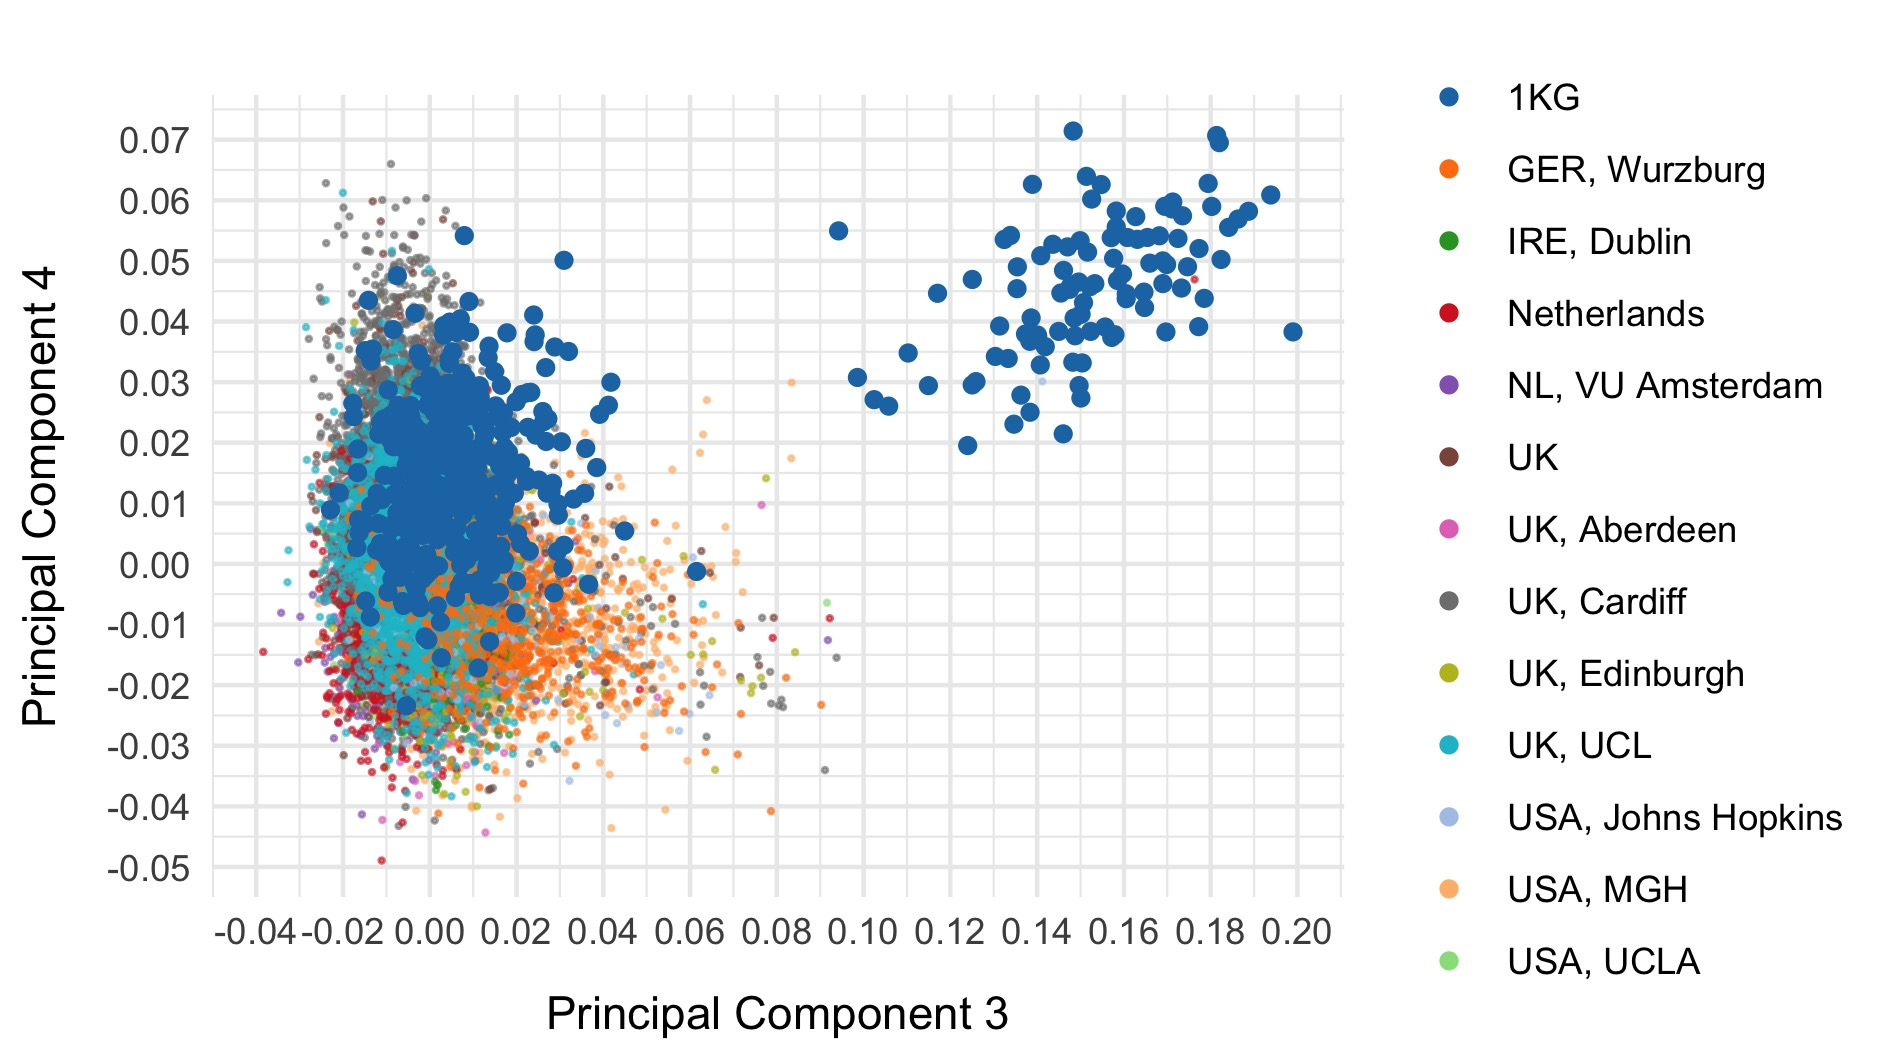
\includegraphics[width=0.5\textwidth]{13_PC3PC4_mainland_EUR_1kg_collection.jpg}}\\
\subfloat{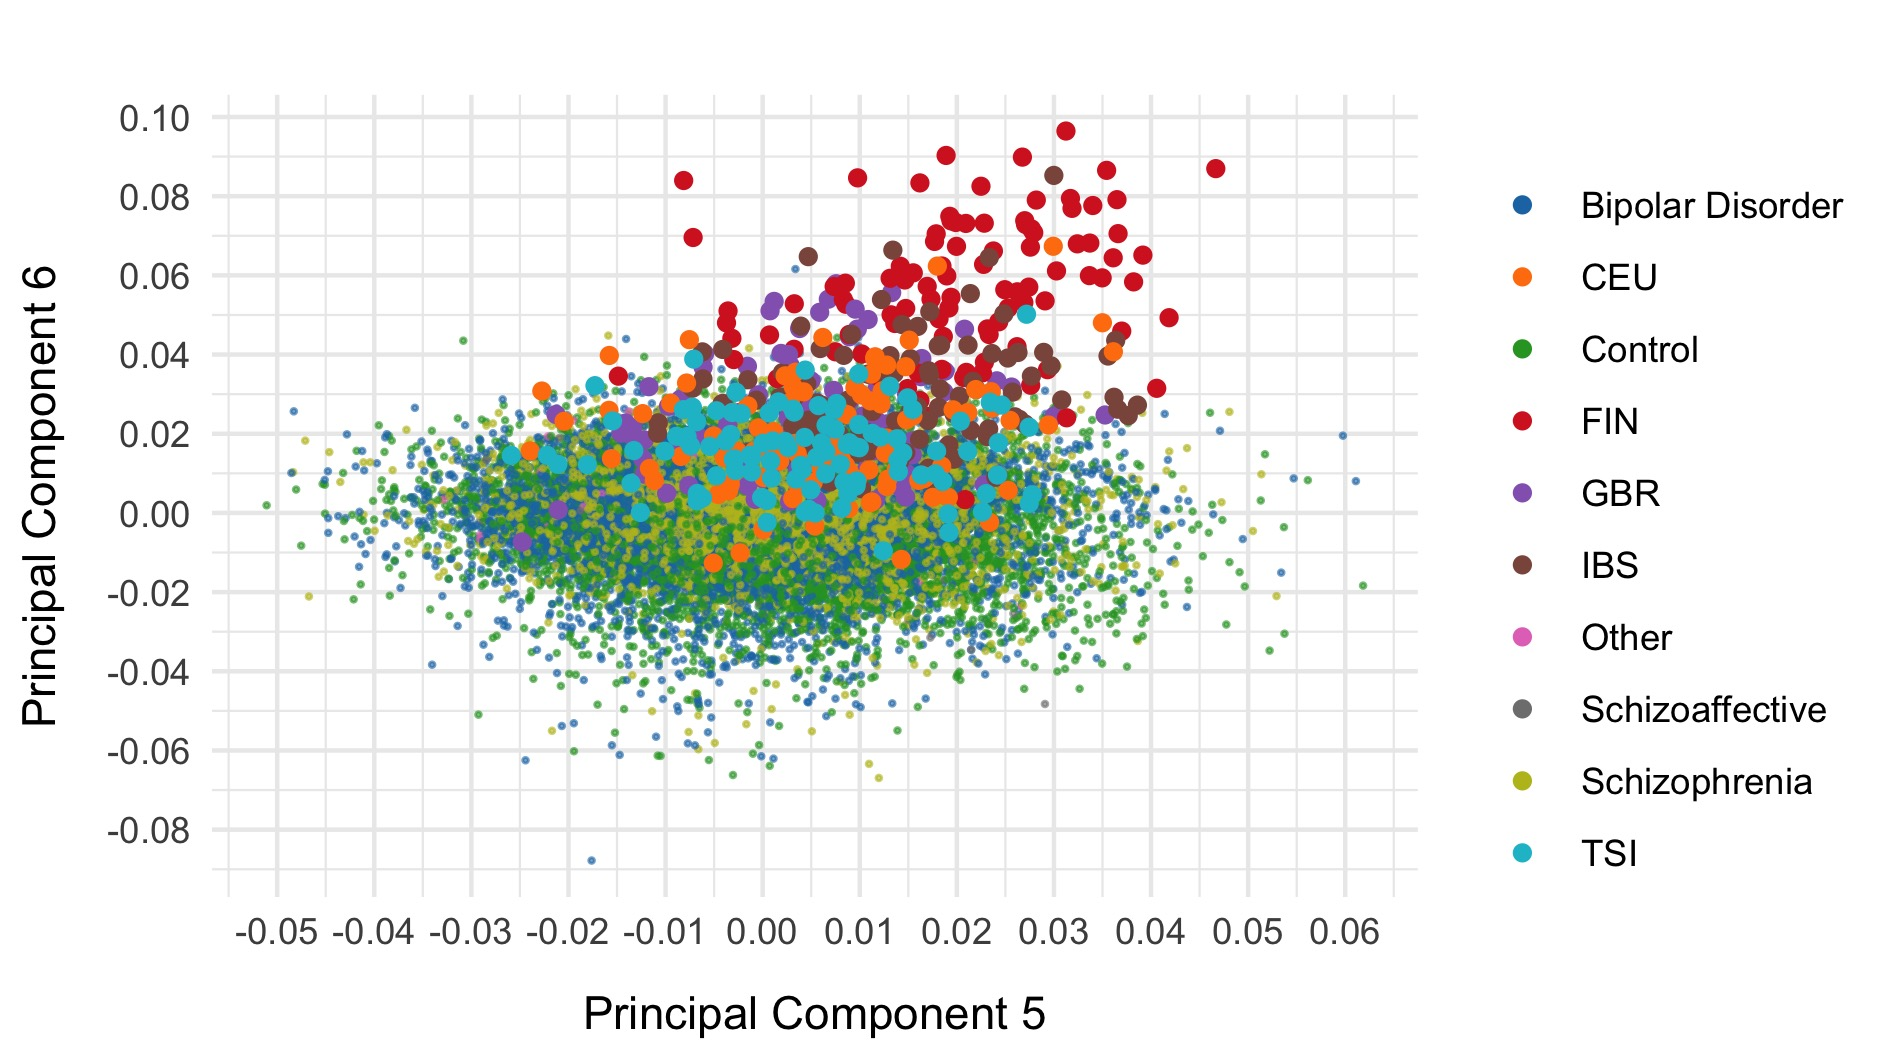
\includegraphics[width=0.5\textwidth]{13_PC5PC6_mainland_EUR_1kg.jpg}}
\subfloat{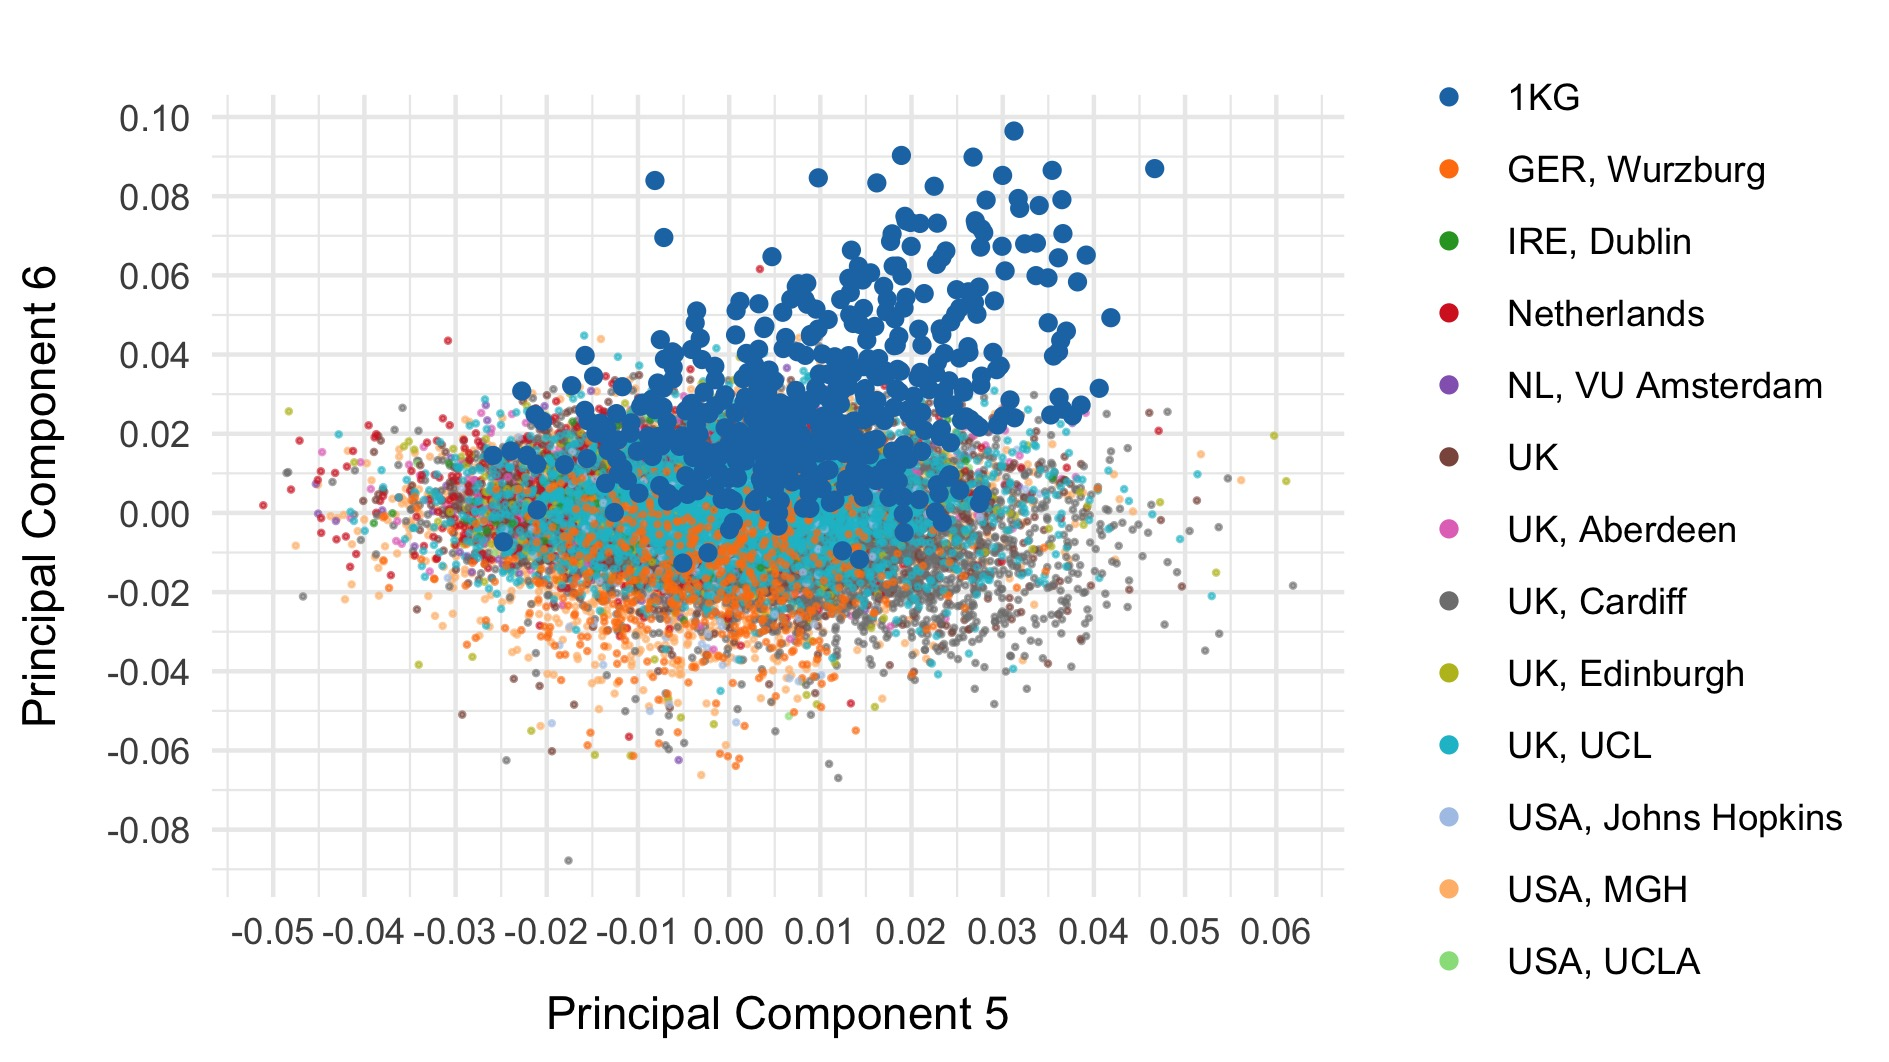
\includegraphics[width=0.5\textwidth]{13_PC5PC6_mainland_EUR_1kg_collection.jpg}}
\caption{PCA of all cohorts except Sweden with 1000 Genomes}
\label{fig:PCA_mainland_EUR_1kg}
\end{figure}

% PCA 1kg SWE
\begin{figure}
\centering
\subfloat{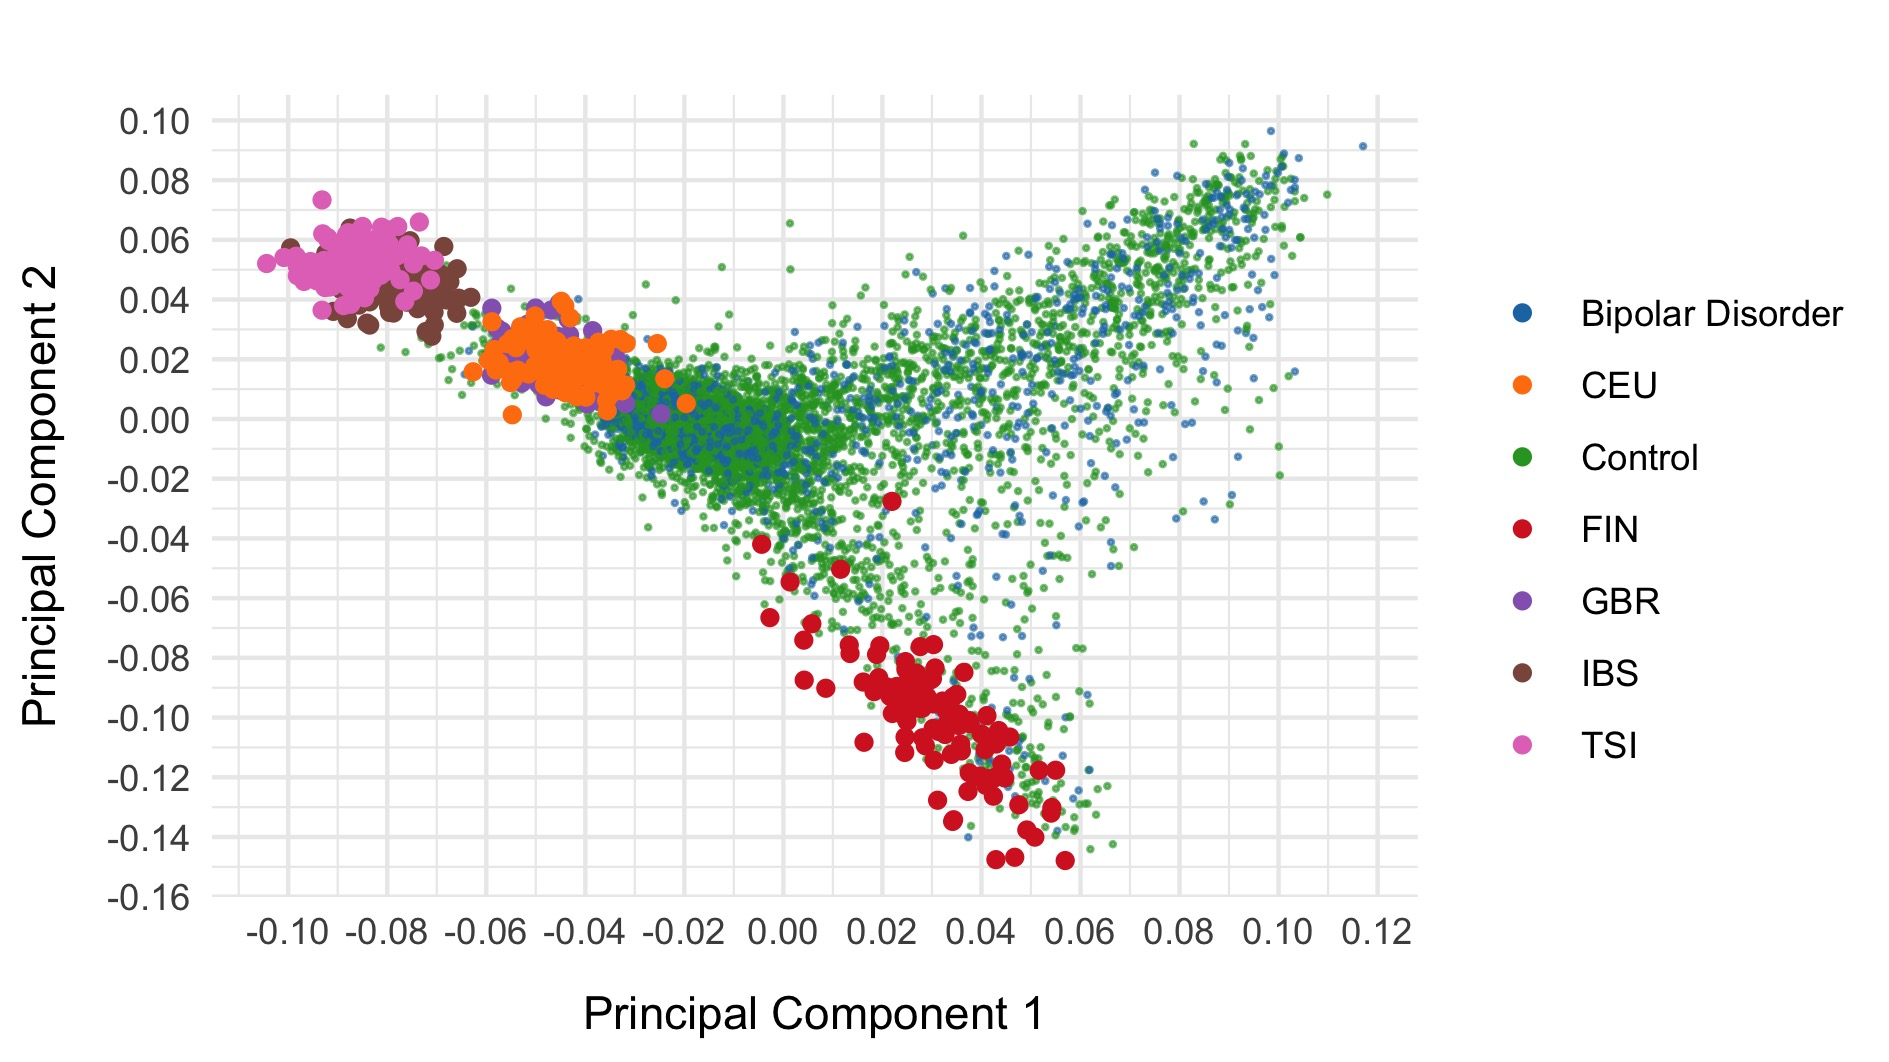
\includegraphics[width=0.5\textwidth]{13_PC1PC2_SWE_1kg.jpg}}
\subfloat{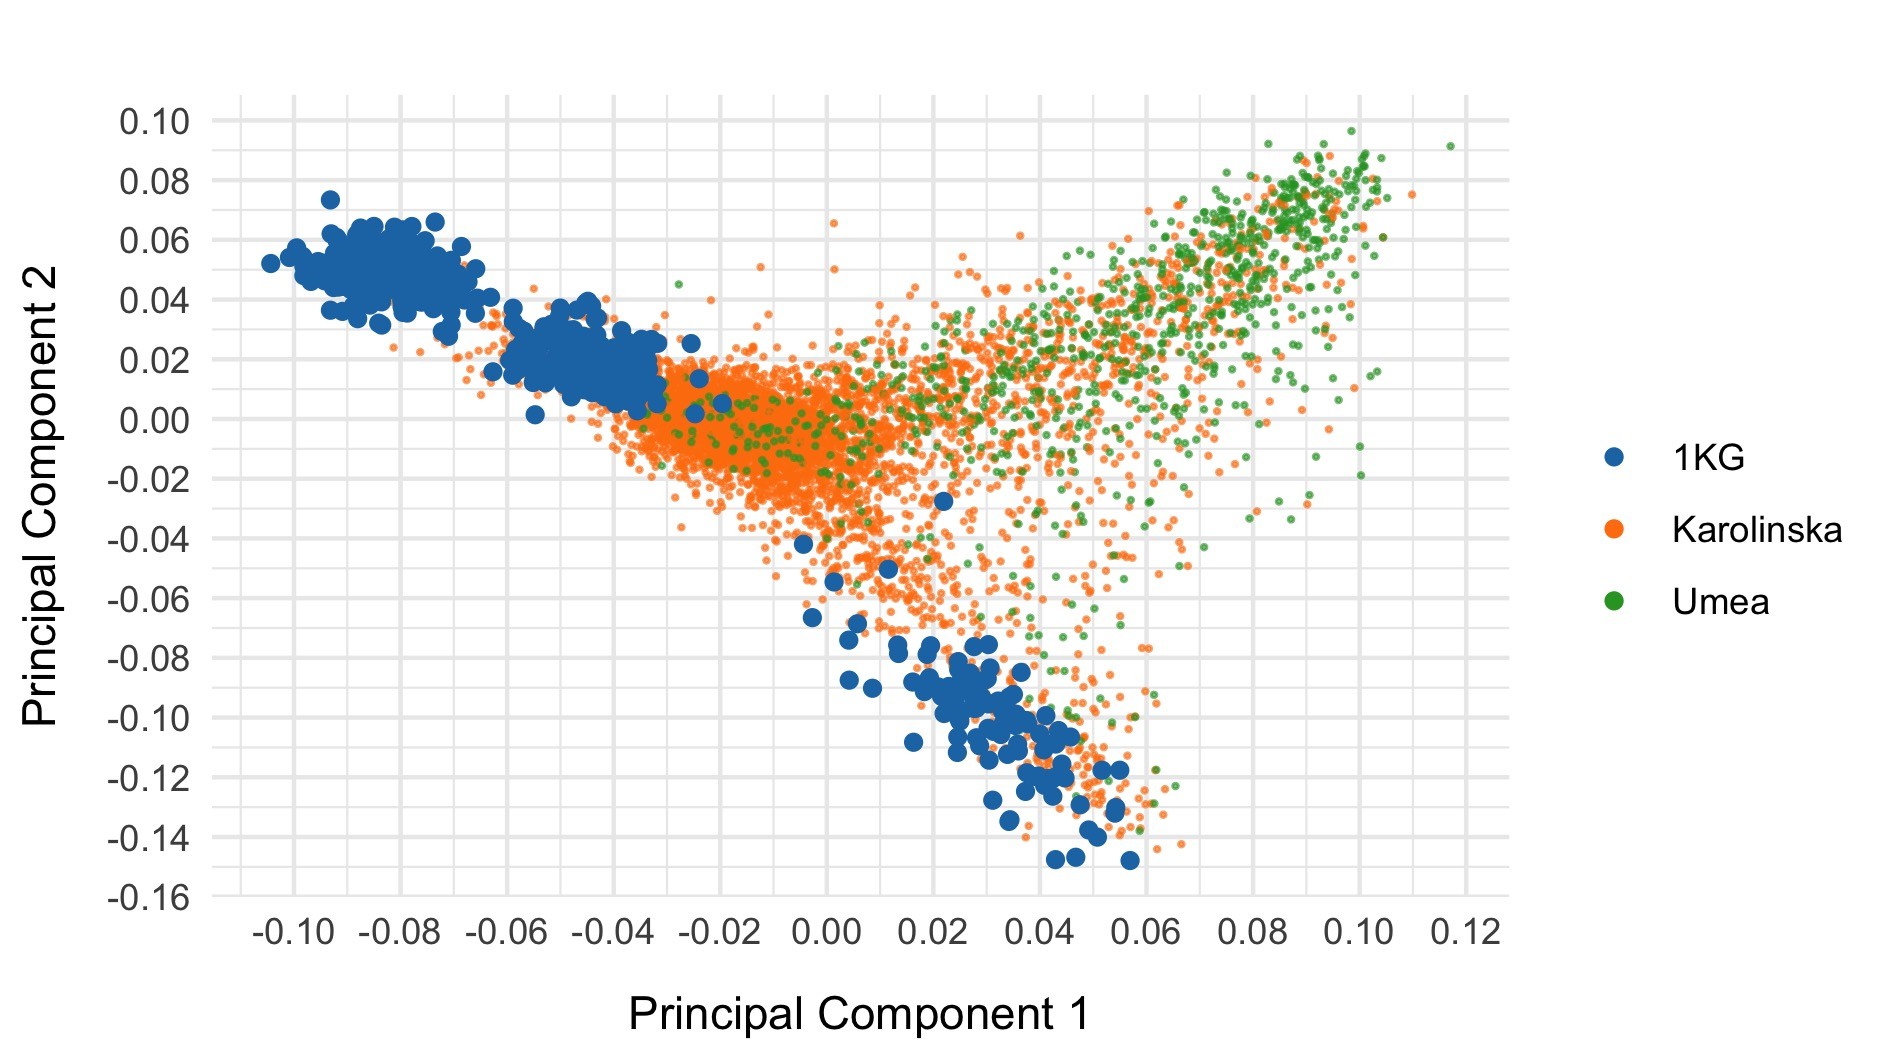
\includegraphics[width=0.5\textwidth]{13_PC1PC2_SWE_1kg_collection.jpg}}\\
\subfloat{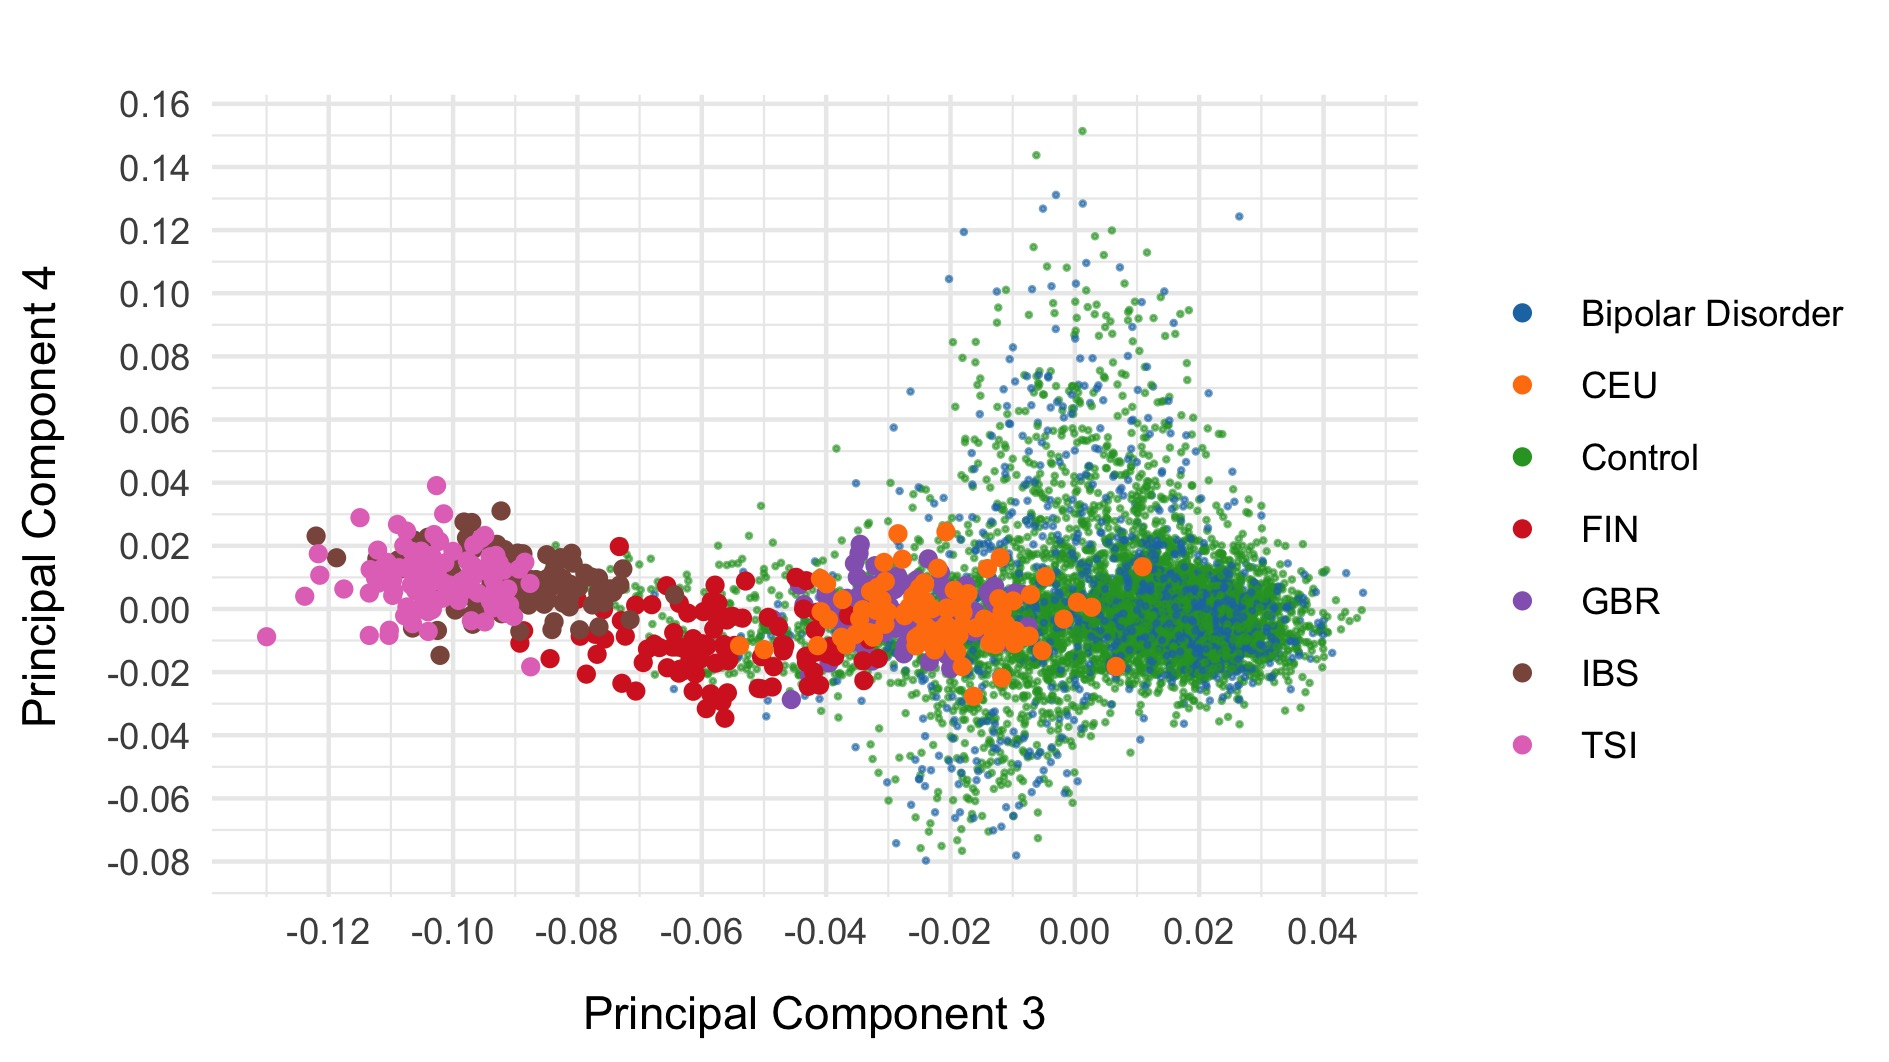
\includegraphics[width=0.5\textwidth]{13_PC3PC4_SWE_1kg.jpg}}
\subfloat{\includegraphics[width=0.5\textwidth]{13_PC3PC4_SWE_1kg_collection.jpg}}\\
\subfloat{\includegraphics[width=0.5\textwidth]{13_PC5PC6_SWE_1kg.jpg}}
\subfloat{\includegraphics[width=0.5\textwidth]{13_PC5PC6_SWE_1kg_collection.jpg}}
\caption{PCA of Swedish cohorts with 1000 Genomes}
\label{fig:PCA_SWE_1kg}
\end{figure}

\begin{figure}
\centering
\subfloat{\includegraphics[width=0.5\textwidth]{15_callRate_cdf.jpg}}
\subfloat{\includegraphics[width=0.5\textwidth]{15_callRate_diff.jpg}}\\
\subfloat{\includegraphics[width=0.5\textwidth]{15_pHWE.jpg}}
\caption{Variant QC}
\label{fig:variant_QC}
\end{figure}

% Variant QC before and after
\begin{figure}
\centering
\subfloat{\includegraphics[width=0.45\textwidth]{16_nSingletonsbyBatchColLocation.jpg}}
\subfloat{\includegraphics[width=0.45\textwidth]{16_nSingletonsbyBatchColPheno.jpg}}\\
\subfloat{\includegraphics[width=0.45\textwidth]{16_rHetHomVarbyBatchColLocation.jpg}}
\subfloat{\includegraphics[width=0.45\textwidth]{16_rHetHomVarbyBatchColPheno.jpg}}\\
\subfloat{\includegraphics[width=0.45\textwidth]{16_rInsertionDeletionbyBatchColLocation.jpg}}
\subfloat{\includegraphics[width=0.45\textwidth]{16_rInsertionDeletionbyBatchColPheno.jpg}}\\
\subfloat{\includegraphics[width=0.45\textwidth]{16_rTiTvbyBatchColLocation.jpg}}
\subfloat{\includegraphics[width=0.45\textwidth]{16_rTiTvbyBatchColPheno.jpg}}\\
\caption{Visualise the impact of variant QC on different metrics.}
\label{fig:variant_QC_impact}
\end{figure}

\begin{figure}
\centering
\subfloat{\includegraphics[width=0.45\textwidth]{18_PC1_PC2_final_PCs.jpg}}
\subfloat{\includegraphics[width=0.45\textwidth]{18_PC3_PC4_final_PCs.jpg}}\\
\subfloat{\includegraphics[width=0.45\textwidth]{18_PC5_PC6_final_PCs.jpg}}
\caption{PCA of pruned cleaned variants and samples.}
\label{fig:final_PCs}
\end{figure}

\end{document}